%%%%%%%%%%%%%%%%%%%%%%%%%%%%%%%%%%%%%%%
%% Modelo TCC - PUC Minas
%% Arquivo Principal	
%%
%% Nome: Marciano Machado Saraiva
%% Data: 2020
%%%%%%%%%%%%%%%%%%%%%%%%%%%%%%%%%%%%%%%

\documentclass{abntpuc}
% \include{pacoteseclass}

% \let\cleardoublepage\clearpage

\usepackage{xcolor}
\usepackage{float}
\usepackage{hyperref}
\usepackage{graphicx}
\usepackage{adjustbox}
\usepackage{tabularx}
\usepackage{cite}
\usepackage{gensymb}
\usepackage{csquotes}
\usepackage{subfig}

\setlength{\cftbeforechapskip}{0pt}
\let\cleardoublepage\clearpage

\usepackage{etoolbox}
\makeatletter
\patchcmd{\scr@startchapter}{\if@openright\cleardoublepage\else\clearpage\fi}{}{}{}
\makeatother

\usepackage{blindtext}

\begin{document}

%%%%%%%%%%%%%%%%%%%%%%%%%%%%%%%%%%%%%%%
%% Modelo TCC - PUC Minas
%% 1 - Capa
%%
%% Nome:
%% Data:
%%%%%%%%%%%%%%%%%%%%%%%%%%%%%%%%%%%%%%%

% --- Campos que formarao: capa, folha de rosto, folha de aprovacao  ---

\curso{Ciência de Dados e Big Data}

\autor{Marciano Machado Saraiva}

\titulo{Previsão da Temperatura do Ar no Brasil Utilizando Estações Meteorológicas e Modelos de Aprendizado de Máquina} % Caixa alta

%\subtitulo{Subt{\'\i}tulo do Trabalho} % Caixa baixa

\cidade{Belo Horizonte}

\ano{2020}

\capa
\trabalho{Trabalho de Conclusão de Curso}

\grau{especialista}

\folharosto{}
% \listafiguras

% \listatabelas

% \listasiglas {
%   \sigla{S1}{Sigla 1}
%  \sigla{S2}{Sigla 2}
%   \sigla{S3}{Sigla 3}
% }

\newpage
\sumario{}
%%\include{3_FolhaDeAprovacao}
%%\include{4_DedicatoriaEAgradecimentos} %(elementos opcionais)
%%\include{4_Epigrafe} %(elemento opcional)
%\include{5_Resumo} 
%\include{6_ListaDeFigurasTabelasESumario} 


\chapter{Introdução}

\section{Contextualização}
As atividades de previsão desempenham um papel fundamental em nossas vidas. Todos os dias, a previsão do tempo nós informa como estará o tempo no dia seguinte, na semana seguinte, e até no mês seguinte. A temperatura, sendo um dos mais importantes parâmetros que são apresentados em previsões do tempo, tem um impacto direto na evaporação, derretimento de neve, geada e um impacto indireto nas condições atmosféricas e precipitação \cite{hansen2006global}. De acordo com recentes estudos sobre os impactos das mudanças climáticas, agricultura, vegetação, recursos hídricos e o turismo são os setores mais afetados diretamente por mudanças de temperatura. Portanto, é necessário prever a temperatura com precisão para evitar perigos inesperados causados pela variação da temperatura, como geadas e secas que podem causar danos financeiros e perdas humanas \cite{kaymaz2005hazards}.

\section{O problema proposto}
Diante desse contexto, este trabalho tem como objetivo prever o comportamento da temperatura média do ar para um intervalo de um ano utilizando séries temporais de temperatura obtidas de estações meteorológicas distribuídas por todo o território brasileiro.

Para facilitar o entendimento do problema e da solução a ser proposta, utilizamos a técnica do 5W's, que consiste em responder as seguintes perguntas:

\textbf{Why?}: Variações de temperatura podem ter impacto direto na produção agrícola, geração de energia, turismo e até na saúde da população, por isso, prever a temperatura com precisão é essencial para evitarmos esses riscos.

\textbf{Who?}: Os dados foram coletados das estações convencionais e automáticas do Instituto Nacional de Meteorologia do Brasil (INMET) e do Laboratório de Meteorologia da Universidade Federal do Vale do São Francisco (LabMet).

\textbf{What?}: Prever o comportamento da temperatura média do ar para um intervalo de um ano utilizando séries temporais de temperatura obtidas de estações mateológicas espalhadas por todo o território brasileiro.

\textbf{Where?}: Estações meteorológicas espalhadas por todo o território brasileiro.  

\textbf{When?}: O conjunto de dados das estações convencionais do INMET contém observações do período de 1961 à 2019. Já as estações automáticas, também do INMET, que começaram a ser implantadas no Brasil a partir no inicio deste século, possui dados de 2000 à 2019. Por último, as estações automáticas do LabMet possui dados de 2007 à 2019. 
\chapter{Coleta de Dados}
 
Neste projeto, utilizamos três diferentes conjuntos de dados meteorológicos. Os dois primeiros conjuntos, que representam maior parte dos dados, foram adquiridos de 265 estações meteorológicas convencionais e 610 estações automáticas vinculadas ao Instituto Nacional de Meteorologia (INMET). O terceiro conjunto de dados foi obtido de 3 estações meteorológicas automáticas administradas pelo Laboratório de Meteorologia da Universidade Federal do Vale do São Francisco (LabMet). Essas estações coletam dados tais como: precipitação, temperatura do ar, umidade relativa do ar, velocidade e direção do vento, radiação solar, dentre outras variáveis. A principal diferença entre esses dois tipos de estações, convencional e automática, é que, as convencionais requerem a presença diária do observador para a coleta dos dados, enquanto as automáticas operam por meio de sensores eletrônicos que alimentam o sistema de aquisição de dados, tendo como principal vantagem o registro contínuo de todas as variáveis. A Figura \ref{figura_estacoes} ilustra a distribuição espacial no território nacional de todas as estações utilizadas neste trabalho. Nas próximas seções descreveremos a cobertura temporal, espacial e as demais informações de cada um dos conjuntos de dados. 

\begin{figure}[H]
    \centering
    \caption{Distribuição espacial das estações meteorológicas utilizadas neste trabalho.}
    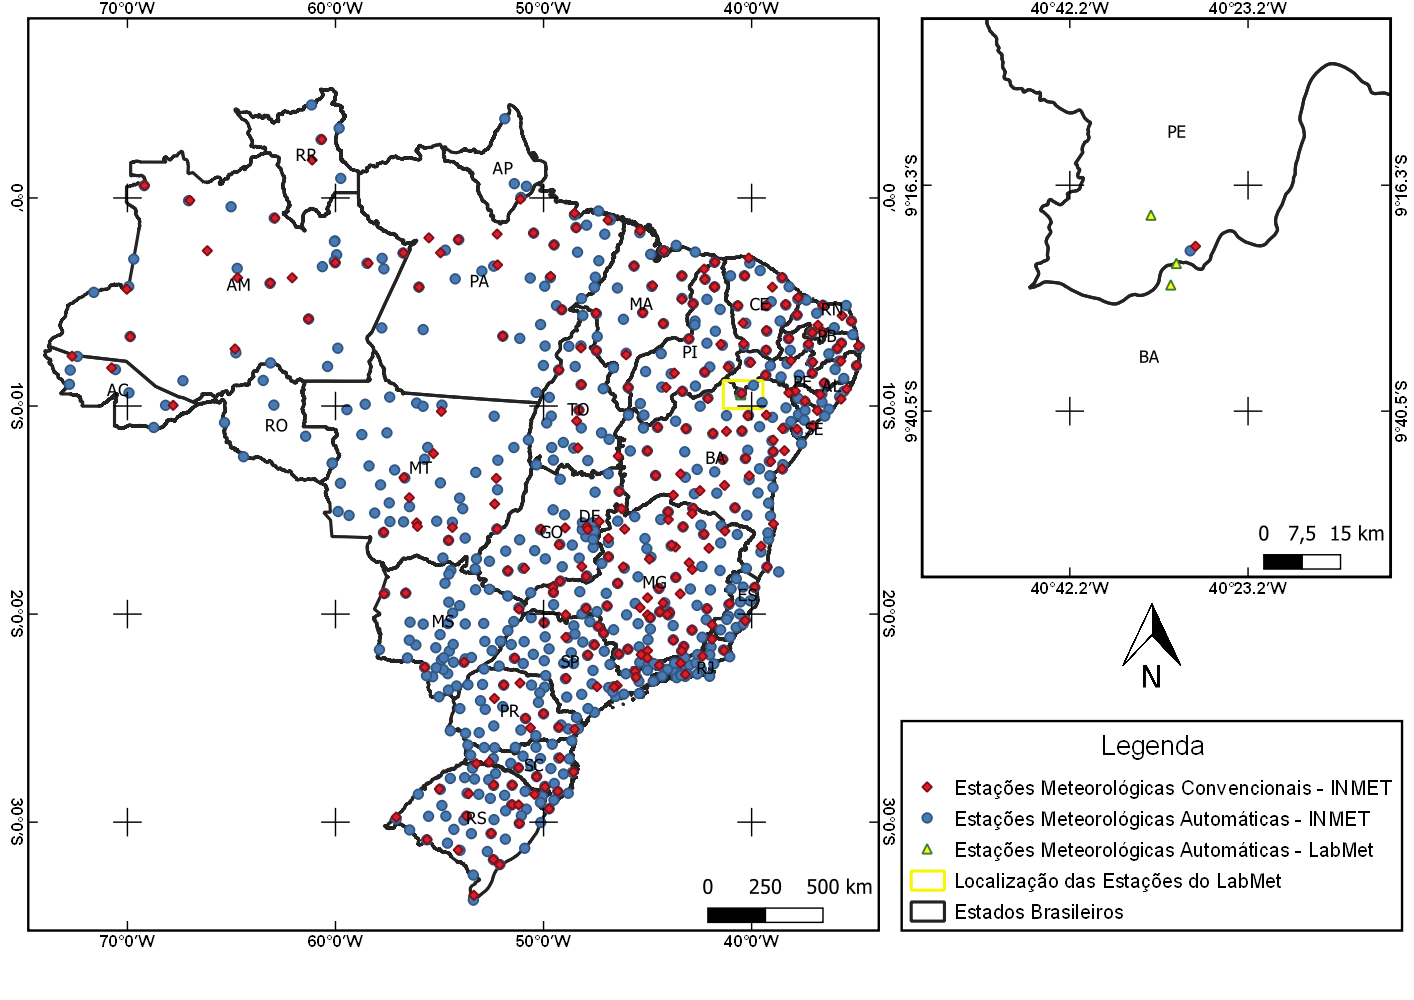
\includegraphics[width=0.9\textwidth]{figuras/espacializacao_estacoes.png}
    \label{figura_estacoes}
\end{figure}

\section{Coleta dos Dados das Estações Meteorológicas Convencionais do INMET}

Distribuídas ao longo de todo o território brasileiro, as estações meteorológicas convencionais vinculadas ao INMET representam os dados com maior série histórica dos três conjuntos, com observações que datam o ano de 1961. Ao todo, foram obtidas mais de 12 milhões de observações coletadas de todas as estações convencionais do INMET para o período de 1961 à 2019. Nas estações convencionais do INMET, cada observação corresponde à uma coleta realizada pelo observador em alguns momentos do dia. 

Os dados das estações convencionais do INMET foram baixados, de forma automatizada, em fevereiro de 2020 a partir do antigo portal do INMET\footnote{O antigo portal do INMET encontrava-se disponível, até a data do download dos dados, no endereço \href{http://www.inmet.gov.br}{http://www.inmet.gov.br}} utilizando a biblioteca Selenium \cite{salunke2014selenium}, versão 3.141.0. Desenvolvemos um script na linguagem de programação Python que percorreu cada uma das estações realizando o \textit{download}, em formato HTML, de todas as variáveis disponíveis na plataforma. A Tabela \ref{tab:variaveis_estacoes_convencionais} apresenta a lista das variáveis disponíveis nas estações convencionais.

\begin{table}[h!]
\caption{Variáveis disponíveis no conjunto de dados das estações meteorológicas convencionais do INMET.}
\label{tab:variaveis_estacoes_convencionais}
\begin{adjustbox}{width=\textwidth}
\begin{tabular}{|l|l|l|} % <-- Alignments: 1st column left, 2nd middle and 3rd right, with vertical lines in between
\hline
\textbf{Nome da coluna} & \textbf{Descrição} & \textbf{Unidade de Medida}\\
\hline
Estacao & Código da Estação  & - \\
\hline
Data & Data da Coleta do Dado  & DD/MM/YYYY\\
\hline
Hora & Hora da Coleta do Dado  & HHMM\\
\hline
Precipitacao & Precipitação Acumulada  & mm\\
\hline
TempBulboSeco  & Temperatura do Bulbo Seco & ºC\\
\hline
TempBulboUmido & Temperatura do Bulbo Úmido & ºC\\
\hline
TempMaxima  & Temperatura Máxima do Ar & ºC\\
\hline
TempMinima  & Temperatura Miníma do Ar & ºC\\
\hline
UmidadeRelativa  & Umidade Relativa do Ar & \% \\
\hline
PressaoAtmEstacao  & Pressão Atmosférico no Nível da Estação & mbar \\
\hline
PressaoAtmMar  & Pressão Atmosférico no Nível do Mar & mbar \\
\hline
DirecaoVento  & Direção do Vento & Código INMET\\
\hline
VelocidadeVento  & Velocidade do Vento & m/s\\
\hline
Insolacao  & Insolação & horas\\
\hline
Nebulosidade & Nebulosidade & décimos \\
\hline
Evaporacao Piche & Evaporação de Piche & mm\\
\hline
Temp Comp Media & Temperatura Compensada Média & ºC\\
\hline
Umidade Relativa Media & Umidade Relativa Média do Ar & \% \\
\hline
Velocidade do Vento Media & Velocidade Média do Vento & m/s\\
\hline
\end{tabular}
\end{adjustbox}
\end{table}

\section{Coleta dos Dados das Estações Meteorológicas Automáticas do INMET}

O segundo conjunto de dados utilizados foram obtidos das estações meteorológicas automáticas vinculadas ao INMET, assim como as convencionais, distribuídas por todo o território nacional. Diferente das estações convencionais que possuem três observações ao longo do dia, e dados desde de 1961, as estações automáticas do INMET coletam dados a cada uma hora desde o ano de 2000. Ao todo, obtivemos quase 55 milhões de observações coletadas de todas as 610 estações meteorológicas automáticas do INMET, para o período de 2000 à 2019.

Os dados de cada uma das estações automáticas foram baixados em agosto de 2020 diretamente do novo portal do INMET\footnote{O novo portal do INMET encontrava-se disponível, até a data do download dos dados, no endereço \href{https://portal.inmet.gov.br/}{https://portal.inmet.gov.br/}} em formato CSV. A Tabela  \ref{tab:variaveis_estacoes_automaticas} apresenta a lista das variáveis disponíveis nos dados baixados.

\begin{table}[h!]
\caption{Variáveis disponíveis no conjunto de dados das estações meteorológicas automáticas do INMET}
\label{tab:variaveis_estacoes_automaticas}
\begin{adjustbox}{width=\textwidth}
\begin{tabular}{|l|l|l|}
\hline
\textbf{Nome da coluna} & \textbf{Descrição} & \textbf{Unidade de Medida}\\
\hline
ESTACAO & Código da Estação  & -\\
\hline
DATA (YYYY-MM-DD) & Data da observação  & YYYY-MM-DD\\
\hline
HORA (UTC) & Hora da observação  & HH\\
\hline
PRECIPITACAO TOTAL HORARIO (mm) & Precipitação Acumulada  & mm\\
\hline
PRESSAO ATMOSFERICA AO NIVEL DA ESTACAO, HORARIA (mB)  & Pressão Atmosférica Instantânea no Nível da Estação & ºC\\
\hline
PRESSAO ATMOSFERICA MAX.NA HORA ANT. (AUT) (mB) & Pressão Atmosférica Máxima & mbar\\
\hline
PRESSAO ATMOSFERICA MIN. NA HORA ANT. (AUT) (mB)  & Pressão Atmosférica Mínima & mbar\\
\hline
RADIACAO GLOBAL (W/m2)  & Radiação Sola Global & W/m2\\
\hline
TEMPERATURA DO AR - BULBO SECO, HORARIA (C)  & Temperatura do Bulbo Seco & ºC \\
\hline
TEMPERATURA DO PONTO DE ORVALHO (C)  & Pressão Atmosférico no Nível da Estação & mbar \\
\hline
PEMPERATURA MAXIMA NA HORA ANT. (AUT) (C)  & Pressão Atmosférico no Nível do Mar & mbar \\
\hline
TEMPERATURA MINIMA NA HORA ANT. (AUT) (C)  & Direção do Vento & Código INMET\\
\hline
TEMPERATURA ORVALHO MAX. NA HORA ANT. (AUT) (C)  & Velocidade do Vento & m/s\\
\hline
TEMPERATURA ORVALHO MIN. NA HORA ANT. (AUT) (C)  & Insolação & horas\\
\hline
UMIDADE REL. MAX. NA HORA ANT. (AUT) (\%) & Nebulosidade & décimos \\
\hline
UMIDADE REL. MIN. NA HORA ANT. (AUT) (\%) & Evaporação de Piche & mm\\
\hline
UMIDADE RELATIVA DO AR, HORARIA (\%) & Temperatura Compensada Média & ºC\\
\hline
VENTO, DIRECAO HORARIA (gr) & Umidade Relativa Média do Ar & \% \\
\hline
VENTO, RAJADA MAXIMA (m/s) & Velocidade Média do Vento & m/s\\
\hline
VENTO, VELOCIDADE HORARIA (m/s) & Velocidade Média do Vento & m/s\\
\hline
\end{tabular}
\end{adjustbox}
\end{table}

\section{Coleta dos Dados das Estações Meteorológicas Automáticas do LabMet}

O último conjunto de dados utilizado foi obtido de 3 estações meteorológicas automáticas localizadas no Vale do Rio São Francisco, entre os estados da Bahia e Pernambuco. Estas estações são administradas pelo Laboratório de Meteorologia da Universidade Federal do Vale do São Francisco (LabMet), que disponibiliam dados diário das estações através de seu portal\footnote{O portal do LabMet encontrava-se disponível, até a data de agosto de 2020, no endereço \href{http://labmet.univasf.edu.br}{http://labmet.univasf.edu.br}}. Ao todo, baixamos, em formato XLS, mais de 9 mil registros disponibilizados para as três estações automáticas entre o período de 2007 à 2020. A Tabela \ref{tab:estacoes_automaticas_labmet} descreve as variáveis contidas no conjunto de dados. 

\begin{table}[h!]
\caption{Descrição dos campos/colunas dos datasets.}
\label{tab:estacoes_automaticas_labmet}
\begin{tabular}{|l|l|l|}
\hline
\textbf{Nome da coluna} & \textbf{Descrição} & \textbf{Unidade de Medida}\\
\hline
Estacao & Código gerado como identificar da estação & - \\
\hline
Data & Data da observação & YYYY-MM-DD\\
\hline
temperatura & Temperatura média do ar & ºC\\
\hline
temperatura maxima & Temperatura máxima do ar & ºC\\
\hline
temperatura minima & Temperatura mínima do ar & ºC\\
\hline
umidade & Umidade relativa média do ar & \% \\
\hline
umidade maxima & Umidade relativa máxima do ar & \% \\
\hline
umidade minima & Umidade relatima mínima do ar & \% \\
\hline
vento maxima 10m & Velocidade máxima do vento diária  & m/s \\
\hline
rad. solar global & Radiação solar global  & MJ/m$^2$/dia\\
\hline
evap. de referencia & Evapotranspiração de Referência & mm/dia\\
\hline
\end{tabular}
\end{table}

\renewcommand{\cleardoublepage}{}
\renewcommand{\clearpage}{}
\vspace{5mm}
\chapter{Processamento e Tratamento dos Dados}

Nesta etapa, nosso principal objetivo foi compatibilizar os diferentes conjuntos de dados, de forma a construir um único conjunto de dados para facilitar o processo de análise e geração dos resultados.

\section{Convertendo todos os dados para um formato de arquivo estruturado}

Os dados obtidos para cada uma das estações meteorológicas convencionais do INMET,  em formato HTML, foram convertidos para o formato CSV utilizando a biblioteca Pandas \cite{mckinney2011pandas} e o kit de ferramentas lxml \cite{behnel2005lxml}. Em seguida, os dados de todas as estações convencionais foram combinados em um único arquivo estruturado em formato CSV. 

Os dados das estações automáticas do INMET já foram obtidos em formato CSV, porém divididos em um arquivo por estação e por ano. Neste conjunto de dados também utilizamos a biblioteca Pandas para combinar todos os dados em um único arquivo, também no formato CSV.

Os dados das estações automáticas do LabMet foram obtidos em formato XLS, um arquivo por variável para cada estação. Cada arquivo de uma determinada variável, para uma determinada estação, possui múltiplas planilhas, cada planilha contém os dados para um determinado ano. Utilizamos a biblioteca Pandas para transformar e agrupar todos os dados das diferentes estações, variáveis e anos em um único arquivo estruturado em formato CSV.


Após esse processo de transformação, obtivemos os conjuntos de dados descritos na Tabela \ref{tab:lista_conjunto_de_dados}.

\begin{table}[H]
\caption{Conjunto de dados utilizados neste trabalho.}
\label{tab:lista_conjunto_de_dados}
\begin{tabular}{|l|c|}
\hline
\textbf{Nome do Conjunto de Dados} & \textbf{Quantidade de Registros}\\
\hline
Estações Meteorológicas Convencionais - INMET  & 12.251.335 \\
\hline
Estações Meteorológicas Automáticas - INMET & 54.840.384 \\
\hline
Estações Meteorológicas Automáticas - LabMet & 11.098 \\
\hline
\end{tabular}
\end{table}

Antes de avançarmos no processo de tratamento e análise dos dados, preparamos um ambiente apropriado para o processamento desse conjunto de dados. 
Em uma máquina com 16 núcleos, 32Gb de memória RAM e 256Gb de SSD, configuramos um ambiente docker\footnote{A configuração docker utilizada para criar o ambiente usado no processamento dos dados está disponível em: \href{https://github.com/saraivaufc/bigdata-docker}{https://github.com/saraivaufc/bigdata-docker}.} com as plataformas Hadoop, versão 3.1.2, e Spark, versão 3.0.1, instaladas. Todos os dados em formato CSV foram ingeridos no sistema de arquivos HDFS do Hadoop para serem processados pelo Spark posteriormente.  

O primeiro conjunto de dados, das estações meteorológicas convencionais do INMET, possui de 2 a 3 registros por dia, dependendo do ano observado, enquanto que as estações automáticas do INMET possui 24 registros por dia (horário), e as estações automáticas do LabMet possuem apenas um único registro por dia (diário). Pensando nisso, decidimos transformar todos os dados para a frequência diária. Essa transformação permitirá juntarmos todos os dados em um único grande conjunto com registros diários das variáveis analisadas. Nas próximas seções descreveremos os passos realizados para realizar essa transformação. 

\section{Transformando os dados das estações convencionais do INMET em registros diários}

Ao analisar as variáveis de temperatura máxima, temperatura mínima e temperatura média nas estações convencionais do INMET, identificamos em torno de 67\% de registros nulos em cada uma das variáveis. Isso se deve, principalmente, pelo fato dessas variáveis estarem presentes em apenas um dos dois ou três registros diários disponibilizados das estações. A temperatura máxima e temperatura média estão presentes no registro das 00:00 horas (UTC) e a temperatura mínima no registro das 12:00 horas (UTC). Com isso, transformamos esse dado para a frequência diária utilizando como registro diário a primeira ocorrência do valor dessas variáveis no dia. Após o procedimento de transformação para dados diários, a quantidade de registro diminuiu de 12.251.335 para 4.224.027 e a porcentagem de dados nulos diminuiu de 67\% para cerca de 6\% nas temperaturas máximas e mínimas, e para próximo de 12\% para a temperatura média. A Tabela \ref{tab:estacoes_convencionais_inmet_dados_nulos} apresenta a quantidade de dados nulos antes e após a transformação para dados diários.  

\begin{table}[H]
\caption{Quantidade de registros nulos antes e após a conversão para dados diários das estações meteorológicas convencionais do INMET}
\label{tab:estacoes_convencionais_inmet_dados_nulos}
\begin{adjustbox}{width=\textwidth}
\begin{tabular}{|l|c|r|r|r|}
\hline
\textbf{Variável} & \textbf{Registros nulos (Qtd.)} & \textbf{Registros nulos (\%)} & \textbf{Registros nulos diários (Qtd.)} & \textbf{Registros nulos diários (\%)} \\
\hline
Temperatura máxima  & 8.300.413 & 67,75\% & 273.105 & 6,46\% \\
\hline
Temperatura mínima & 8.292.199 & 67,68\% & 264.891 & 6,27\% \\
\hline
Temperatura média & 8.528.574 & 69,61\% & 501.266 & 11,86\% \\
\hline
\end{tabular}
\end{adjustbox}
\end{table}

\section{Transformando os dados das estações automáticas do INMET em registros diários}

Nas estações meteorológicas automáticas do INMET, os valores nulos estão indicados com o valor -9999, então o primeiro passo foi convertermos todos os valores -9999 para o valor "NULO". Em seguida, realizamos a contagem dos valores nulos dos dados horários das variáveis Temperatura Máxima, Temperatura Mínima e Temperatura do Bulbo seco. Utilizamos a temperatura do bulbo seco horária para estimar a temperatura média do ar diária. Esta primeira análise indicou que apenas aproximadamente 4\% dos dados das variáveis analisadas estavam com valores nulos. Os dados estão disponíveis originalmente na periodicidade horária, para convertermos para dados diários de temperatura máxima, mínima e média, calculamos o máximo valor da temperatura máxima, o mínimo valor da temperatura mínima e a média dos 24 valores da temperatura do bulbo seco, respectivamente. Após a conversão dos dados horários para dados diários, a quantidade de registros passaram de 54.840.384 para 2.072.346, e a quantidade de dados nulos passaram de aproximadamente 4\% para cerca de 6\% nos dados diários. O aumento em proporção dos dados nulos na escada diária indica que a escala horária tinha muitos dados nulos agrupados um mesmo mesmo período de 1 dia. 


\begin{table}[H]
\caption{Quantidade de registros nulos antes e após a conversão para dados diários das estações meteorológicas automáticas do INMET}
\label{tab:estacoes_convencionais_inmet_dados_nulos}
\begin{adjustbox}{width=\textwidth}
\begin{tabular}{|l|c|r|r|r|}
\hline
\textbf{Variável} & \textbf{Registros nulos (Qtd.)} & \textbf{Registros nulos (\%)} & \textbf{Registros nulos diários (Qtd.)} & \textbf{Registros nulos diários (\%)} \\
\hline
Temperatura máxima  & 496.231 & 4,05\% &125.226 & 6,04\% \\
\hline
Temperatura mínima & 496.396 & 4,05\% & 125.226 & 6,04\% \\
\hline
Temperatura média & 493.102 & 4,02\% & 125.014 & 6,03\% \\
\hline
\end{tabular}
\end{adjustbox}
\end{table}

\section{Registros diários das estações automáticas do LabMet}

Por já estarem na frequência diária, os dados das estações meteorológicas automáticas do LabMet não sofreram alterações. Verificando a ocorrência de valores nulos, não identificamos nenhum valor nulo da variável de temperatura miníma, um registro nulo na temperatura máxima, e dois registros nulos na variável da temperatura média. 

\section{Eliminando valores inconsistentes}

Esta etapa verifica a ocorrência de dados inconsistentes. Geralmente, esses dados são aqueles gerados por erros de leituras dos sensores, com problemas de calibração ou com defeitos. Baseado em \citeonline{baba2014correccao}, subdividimos as inconsistências em três grupos, inconsistências de limites, inconsistências lógicas, e inconsistências temporais. 

\begin{itemize}
	\item Inconsistência de limites: identifica valores que não respeitam os límites básicos da variável representada, ou seja, um valor fisicamente impossível de ser obtido. Nos dados de temperatura consideramos como inconsistência, para o Brasil, valores menores que -30ºC e maiores que 50ºC. Qualquer valor fora do intervalo estaria incorreto, pois representaria um valor impossível para a variável em questão.
	\item Inconsistências lógicas: quando temos dados de temperatura máxima, média e mínima referentes a um intervalo de tempo monitorado, estes dados devem respeitar sua condição lógica básica, ou seja, o valor de temperatura média para um período não pode ser maior que a temperatura máxima ou menor que a temperatura mínima deste mesmo período. Do contrário, esses valores serão considerados inconsistentes.     
	\item Inconsistências temporais: identifica valores inconsistentes baseado em seus valores históricos. Para esta análise, foi utilizada a metodologia elaborada por \cite{mateo2008design}, em que consiste em determinar a consistência do dado avaliado baseado no valor do dia anterior, no valor do dia  seguinte e nos dados referentes aos três dias (anterior, corrente, posterior) do ano anterior. Se o valor do dado analisado se afastar da média dos valores analisados 3 vezes o valor do desvio padrão, este valor pode indicar problemas de leituras.  
\end{itemize}

Ao final desta etapa, utilizamos os dados de temperatura máxima e mínima para validar o dado de temperatura média, mas após esta etapa eliminares os dados de temperatura máxima e mínima e passamos a trabalhar apenas com a temperatura média. Antes de eliminar os valores inconsistentes, nosso conjunto de dados resultado da combinação de todas as bases de dados continha 6.300.381 registros com 619.192 destes nulos, ou seja, 9,82\% de todos os registros. Após a eliminação dos valores inconsistentes a quantidade de registros nulos subiu para 958.992, representando 15,22\% do dado. 

\chapter{Análise e Exploração dos Dados}

Nesta etapa da analise dos dados, uma das primeiras informações que levantamos foi a quantidade de estações por estado. Na Figura \ref{fig:estacoes_por_estado} podemos observar que os estados com maior quantidade de estações meteorológicas instalados são, em primeiro lugar, Minas Gerais com 116 estações, seguido pelos estados da Bahia com 78 estações,  Rio Grande do Sul com 62 estações e São Paulo com 54 estações. Em contrapartida, os estados de Rondônia,  Roraima, e Amapá possuem apenas 7, 5 e 5 estações, respectivamente.  

\begin{figure}[H]
    \centering
    \caption{Distribuição, por estado, das estações meteorológicas analisadas.}
    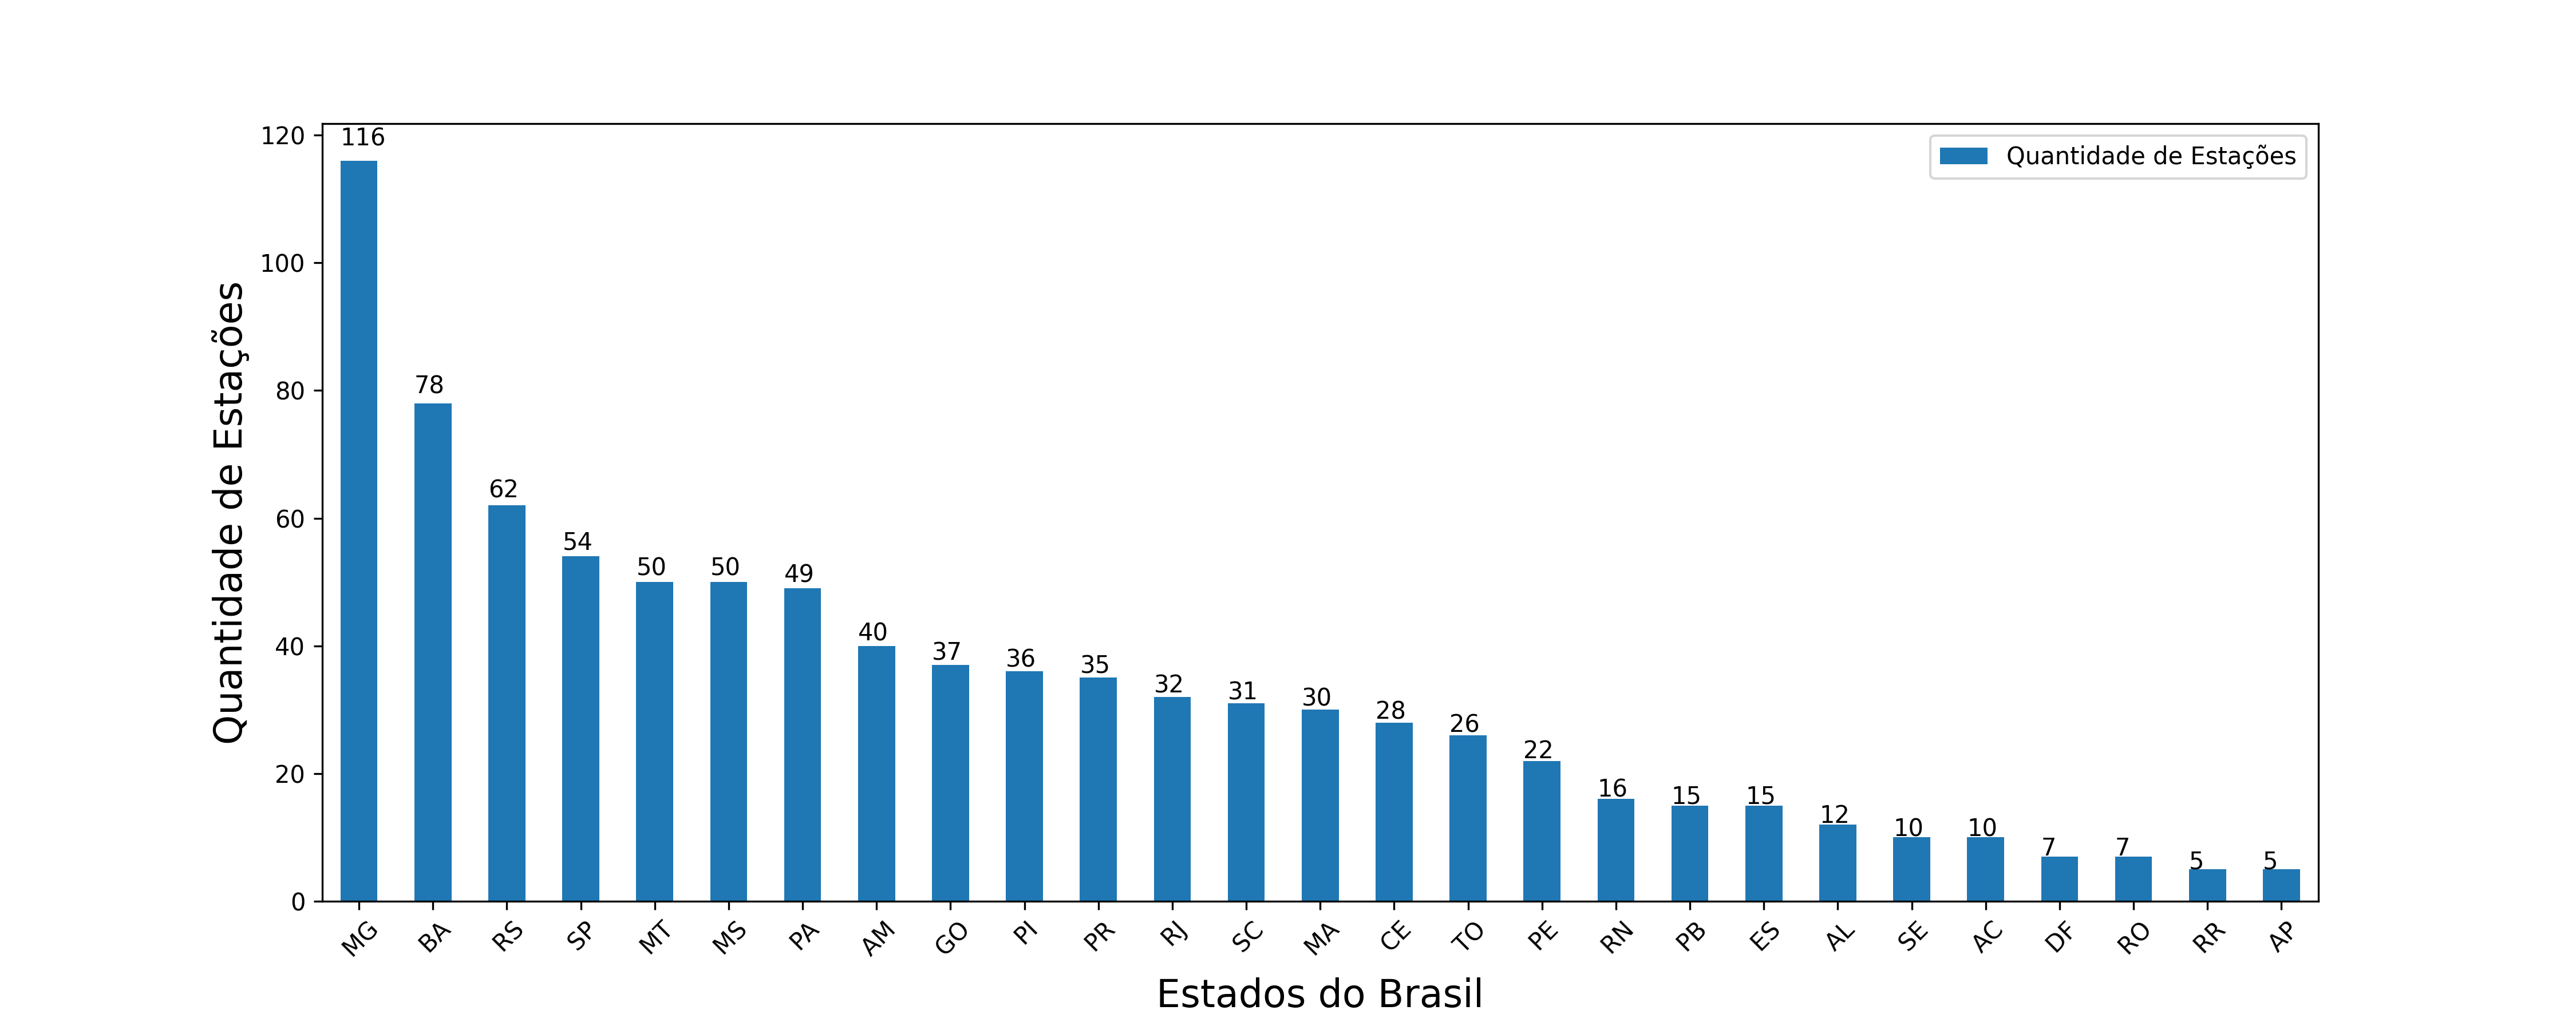
\includegraphics[width=0.9\textwidth]{figuras/estacoes_por_estado.png}
    \label{fig:estacoes_por_estado}
\end{figure}

Dentre estas estações analisadas, há estações convencionais com dados disponíveis deste do ano de 1961, até estações automáticas recentemente instaladas, com dados apenas para os últimos anos. Por isso, é importante entendermos como varia a disponibilidade de dados ao longo de todo o período afim de nos orientarmos melhor na criação dos nossos modelos. Para isso, apresentamos na Figura \ref{fig:disponibilidade_historica_de_dados} a disponibilidade das observações das estações ao longo de todo o período analisado. Podemos observar que a partir do ano de 2002 há um crescimento na quantidade de dados disponíveis, com maiores crescimentos nos anos de 2007 e 2008. Isso se deve pela adoção ao processo de automação de dados meteorológicos através de monitoramento por estacões automáticas que surgiu no Brasil no inicio deste século.  

\begin{figure}[H]
    \centering
    \caption{Disponibilidade de dados ao longo de todo o período analisado.}
    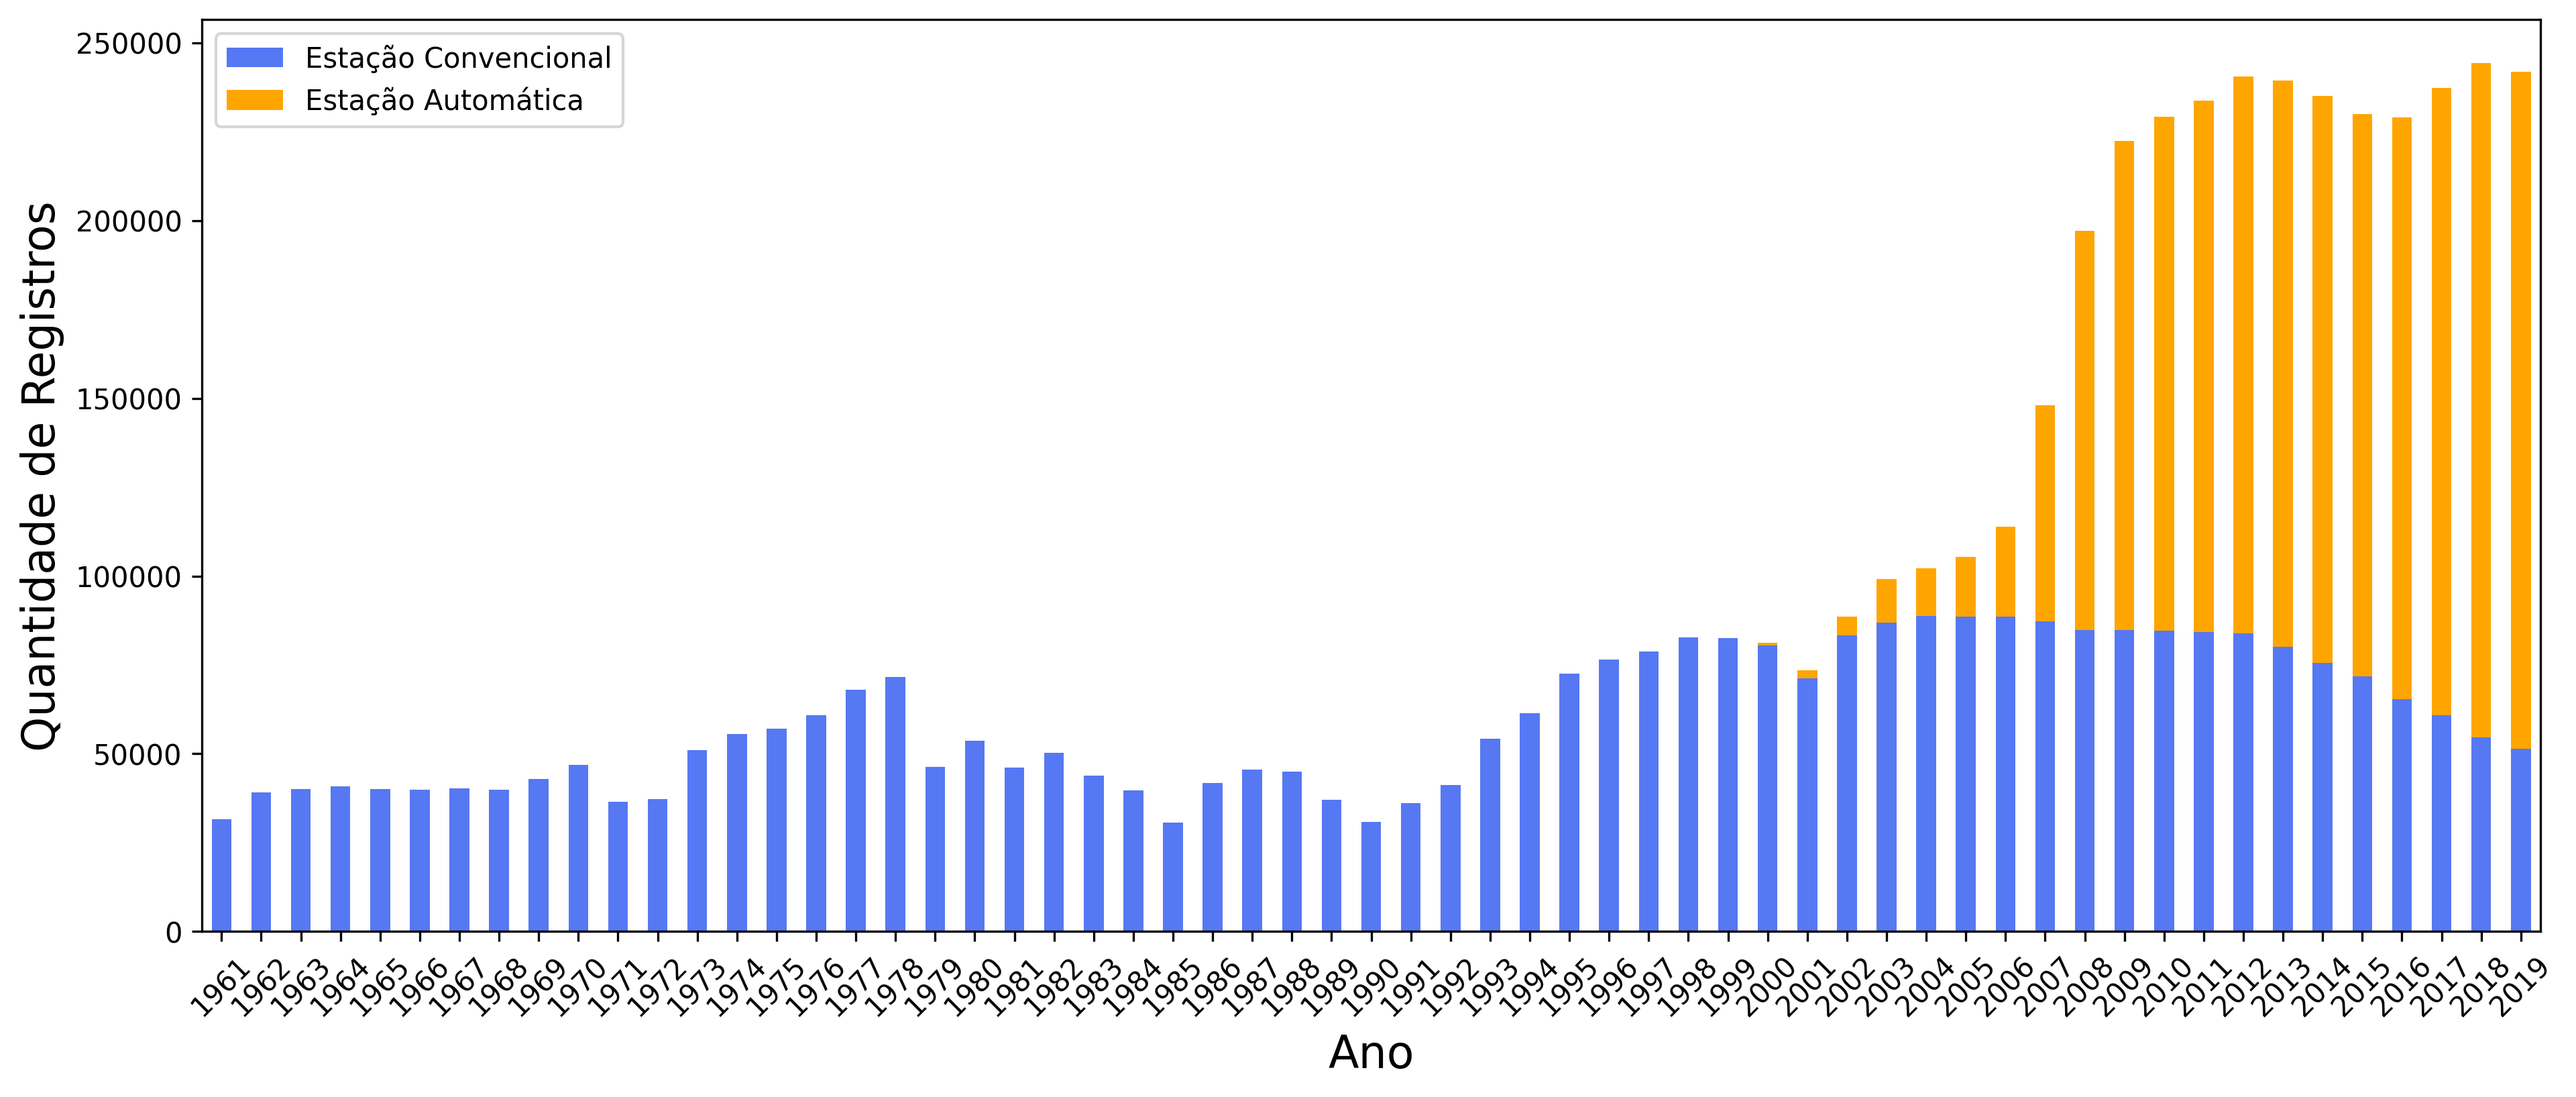
\includegraphics[width=0.9\textwidth]{figuras/disponibilizade_historica_de_dados.png}
    \label{fig:disponibilidade_historica_de_dados}
\end{figure}

Ainda observando a Figura \ref{fig:disponibilidade_historica_de_dados}, é possível observarmos uma declínio de dados em alguns anos específicos. Por exemplo, de 1978 para 1979 houve uma diminuição na quantidade de dados disponíveis. Para entender melhor essa variação, e avaliar melhor a quantidade de dados que ficaram ausentes no conjunto final, adicionamos na Figura \ref{fig:dados_ausentes_ao_longo_anos} também a quantidade de dados que estão ausentes para os anos apresentados.

\begin{figure}[H]
    \centering
    \caption{Quantidade de nulos ao longo de todo o período analisado.}
    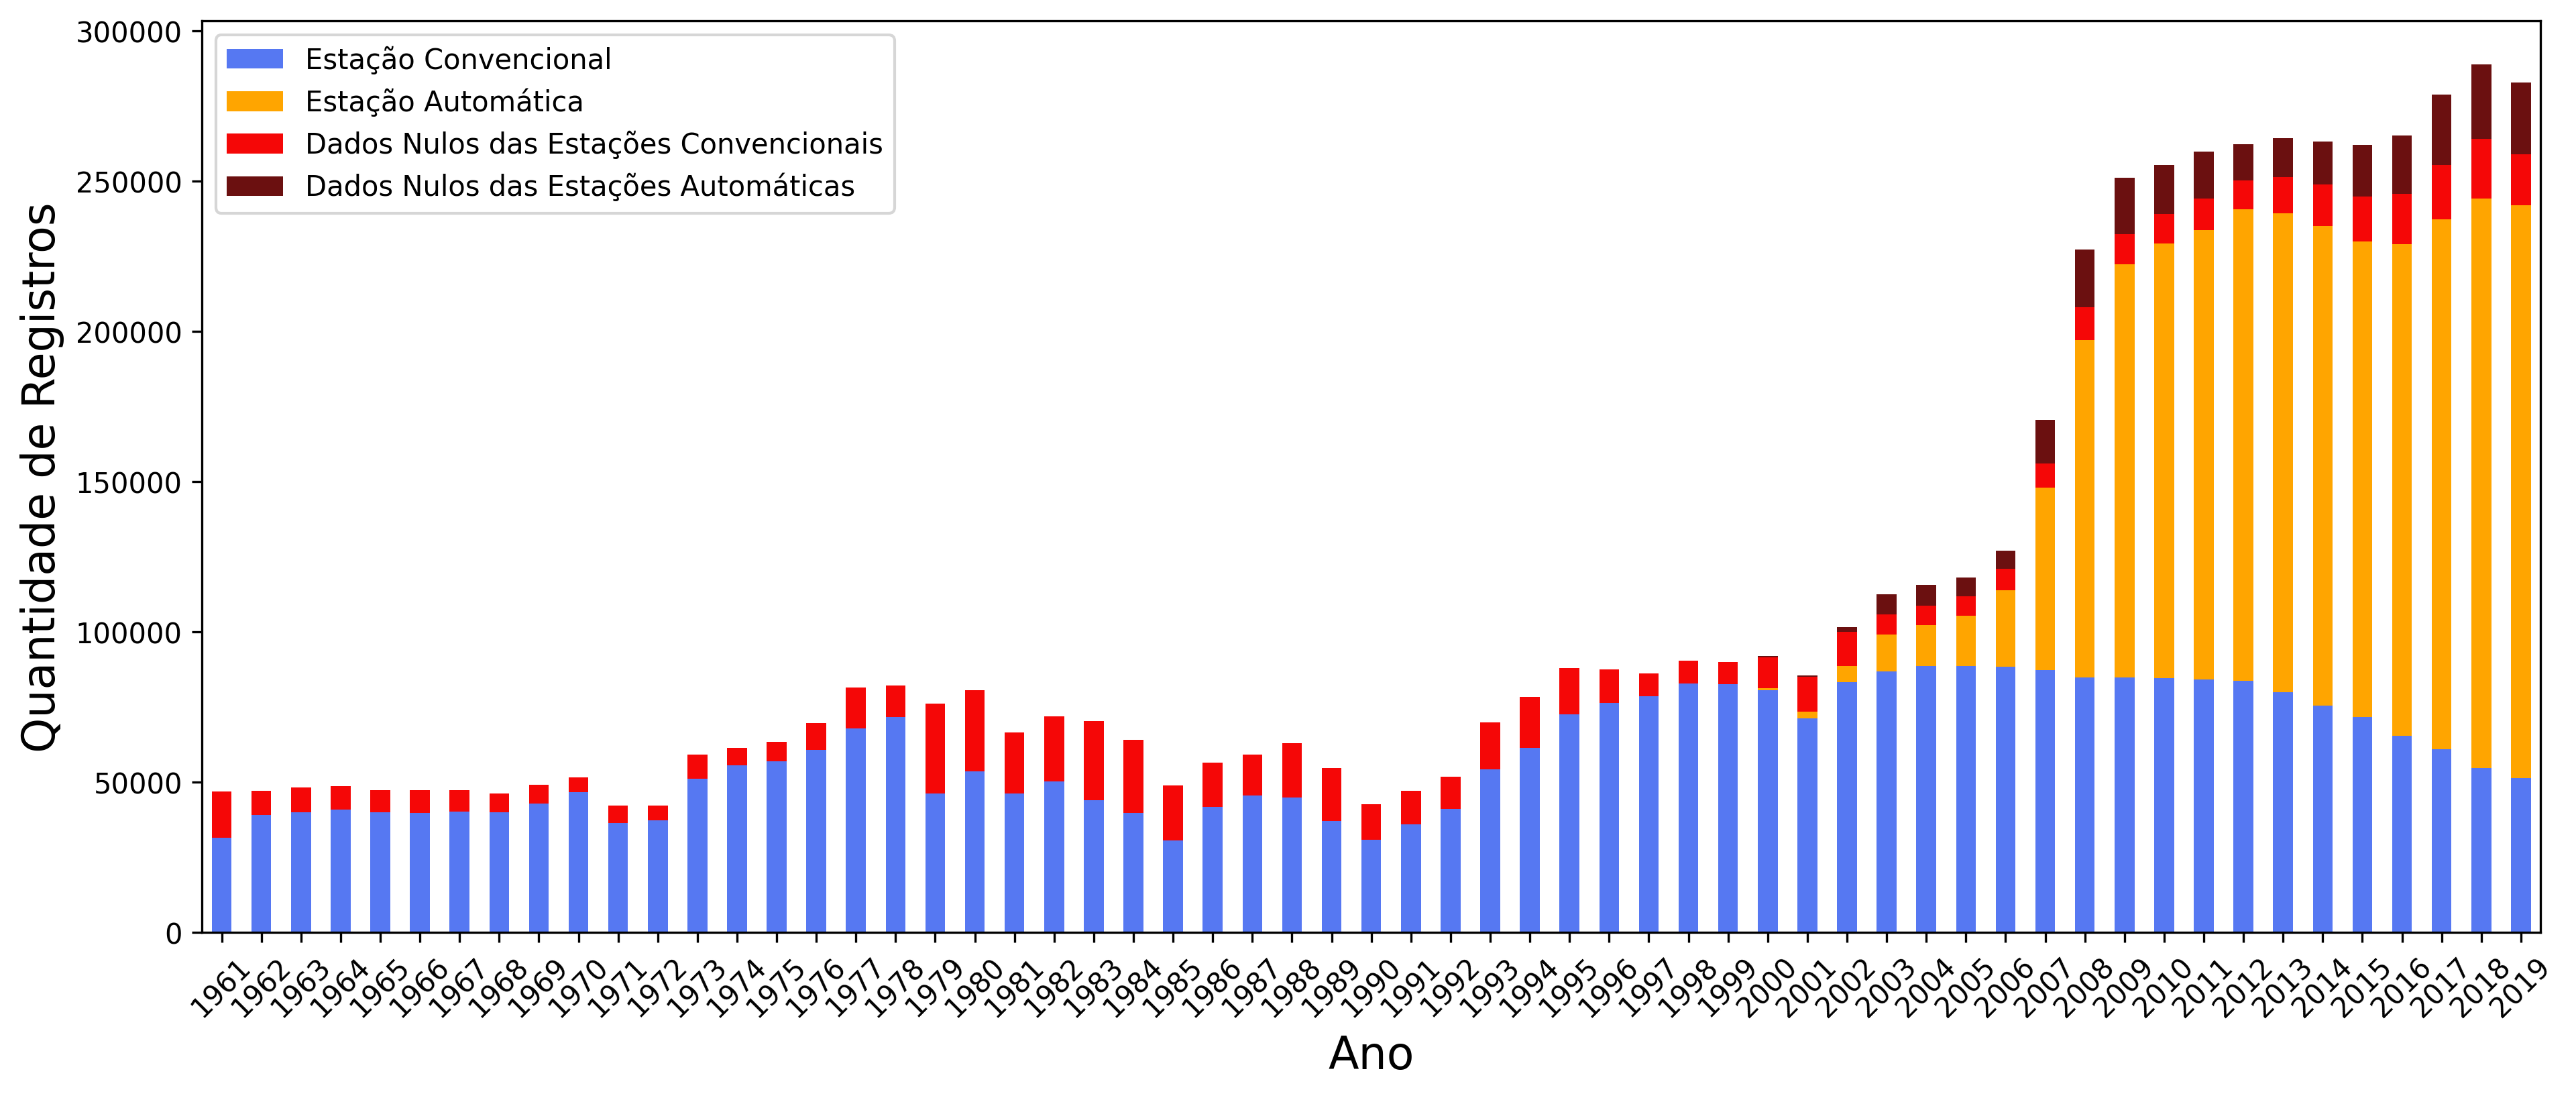
\includegraphics[width=0.9\textwidth]{figuras/dados_ausentes_ao_longo_anos.png}
    \label{fig:dados_ausentes_ao_longo_anos}
\end{figure}

A ausência de dados em estações meteorológicas pode ser causada por várias razões, entre elas mudança geográfica da estação, mudança no instrumental, tempo de observação e práticas observacionais utilizadas \cite{oliveira2019estaccao}. 

Uma informação que também é importante identificarmos nos dados, é se, valores extremos que ocorreram, de fato, na realidade, não foram removidos durante o processo de limpeza dos dados.
Para isso, ilustramos nas Figuras \ref{fig:estacoes_convencionais_maiores_temperaturas} e \ref{fig:estacoes_convencionais_menores_temperaturas} os recordes de temperatura máxima e mínima para as estações convencionais do INMET, pois estas são as que possuem maior série histórica e maior consistência dos valores. 

\begin{figure}[H]
    \centering
    \caption{Recorde das maiores temperaturas já registradas no período de 1961 a 2019 nas estações convencionais do INMET.}
    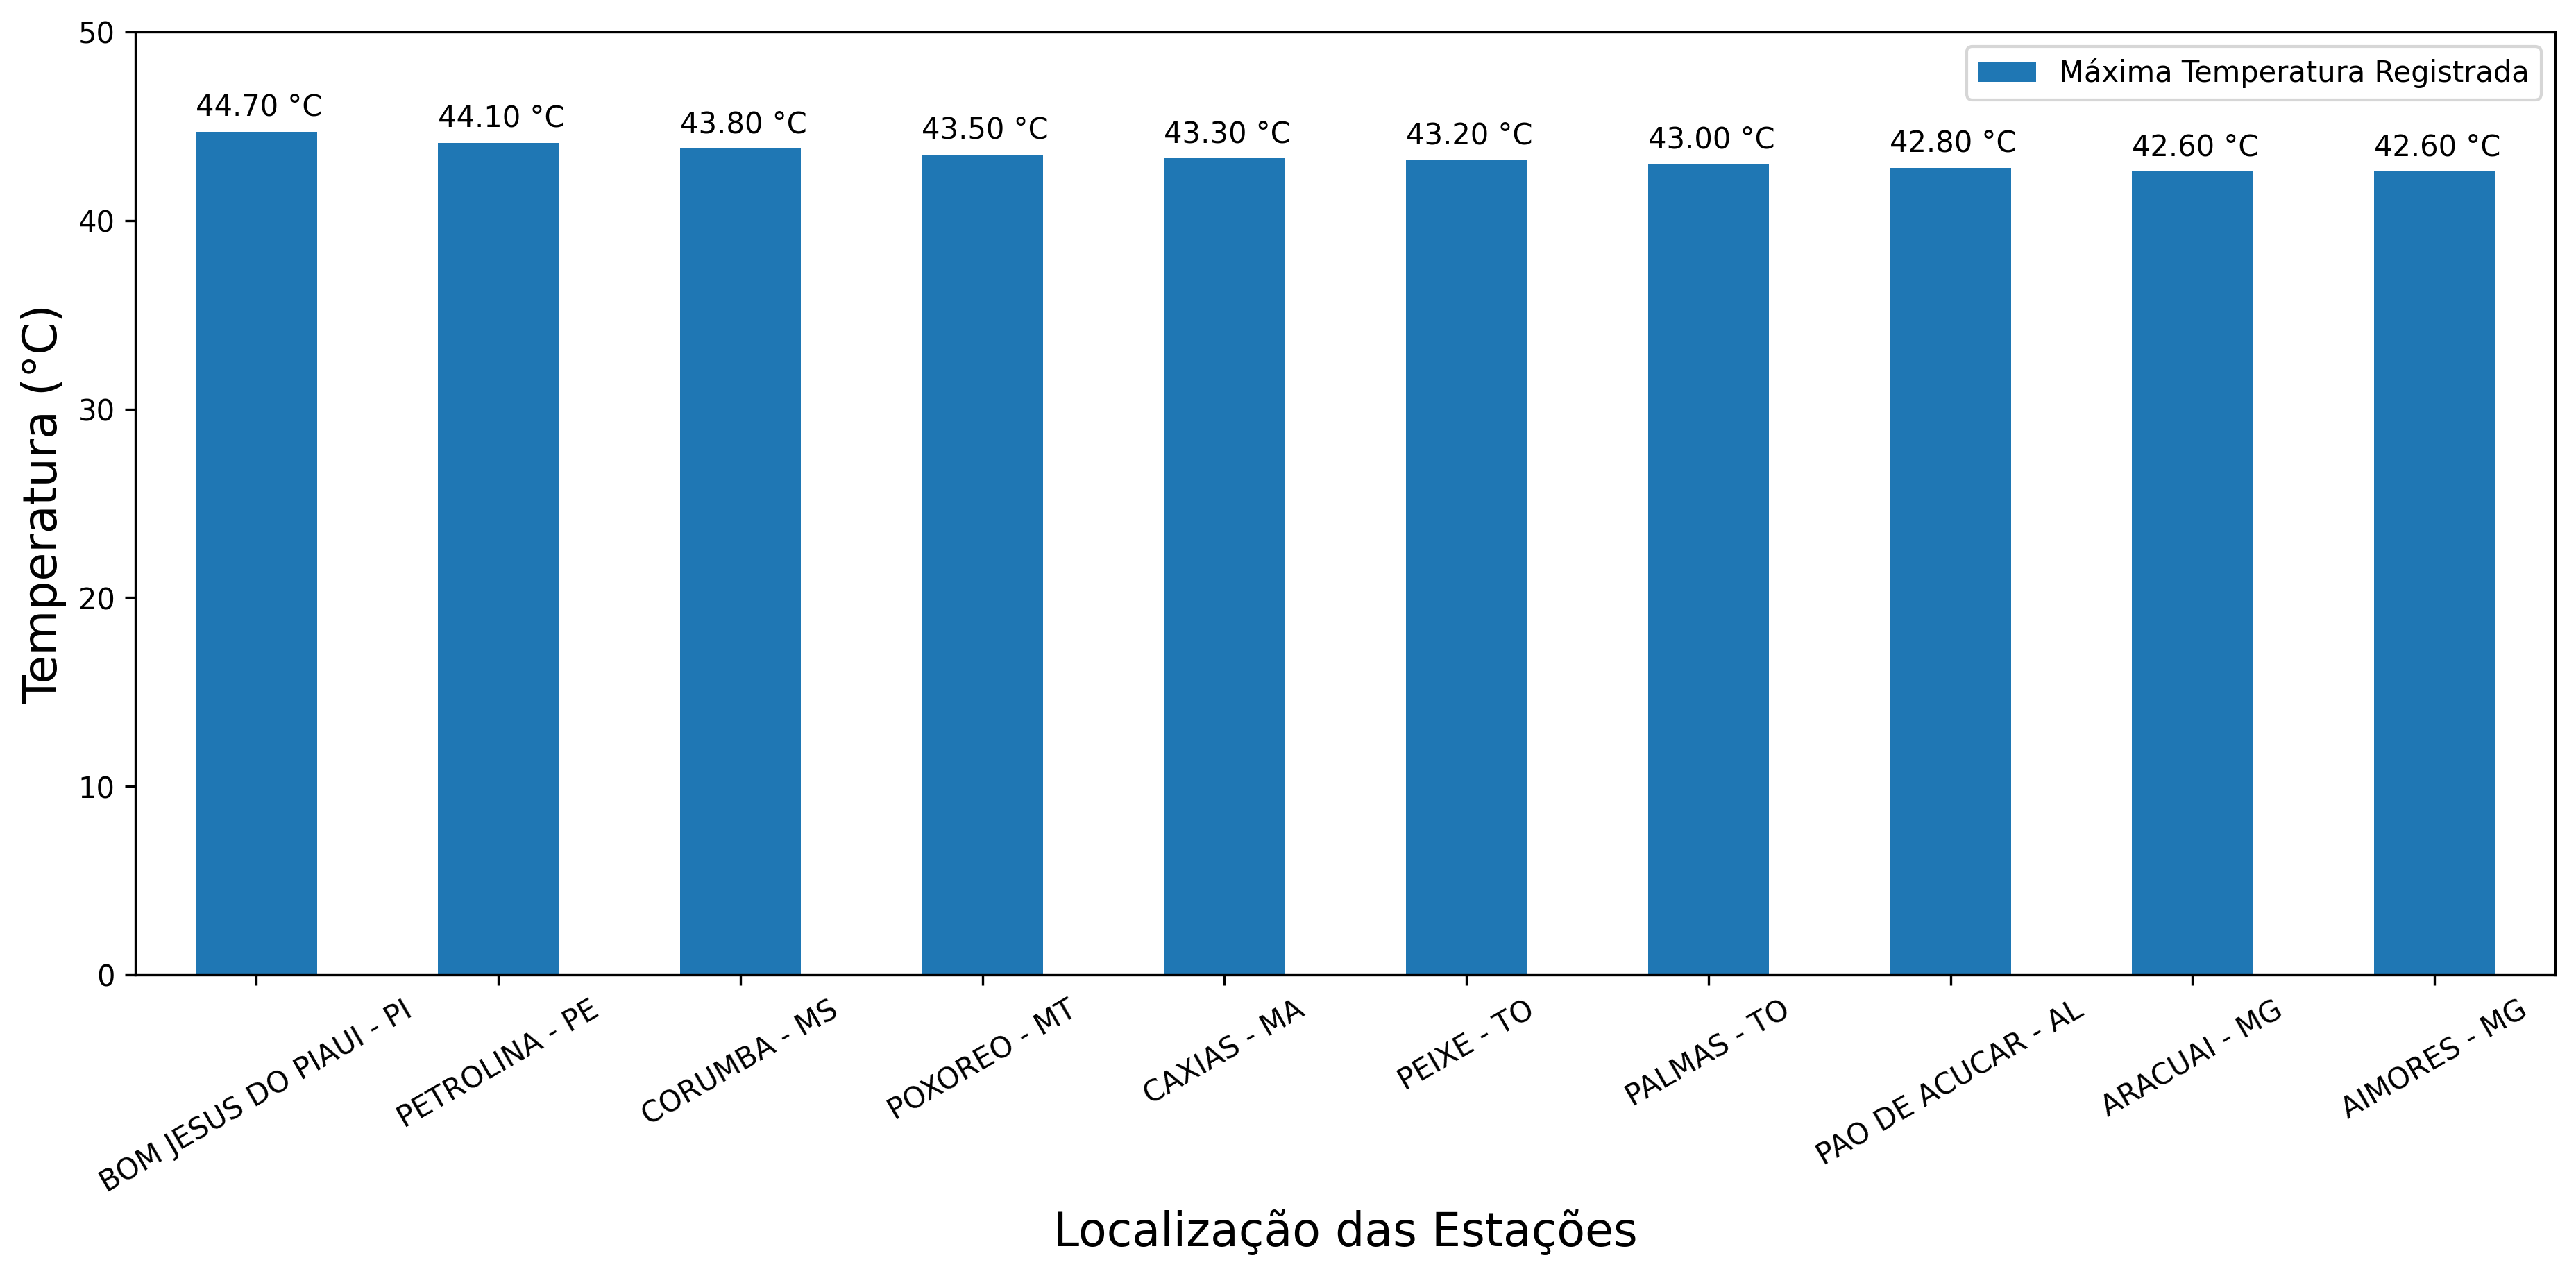
\includegraphics[width=0.9\textwidth]{figuras/estacoes_convencionais_maiores_temperaturas.png}
    \label{fig:estacoes_convencionais_maiores_temperaturas}
\end{figure}

\begin{figure}[H]
    \centering
    \caption{Recorde das menores temperaturas já registradas no período de 1961 a 2019 nas estações convencionais do INMET.}
    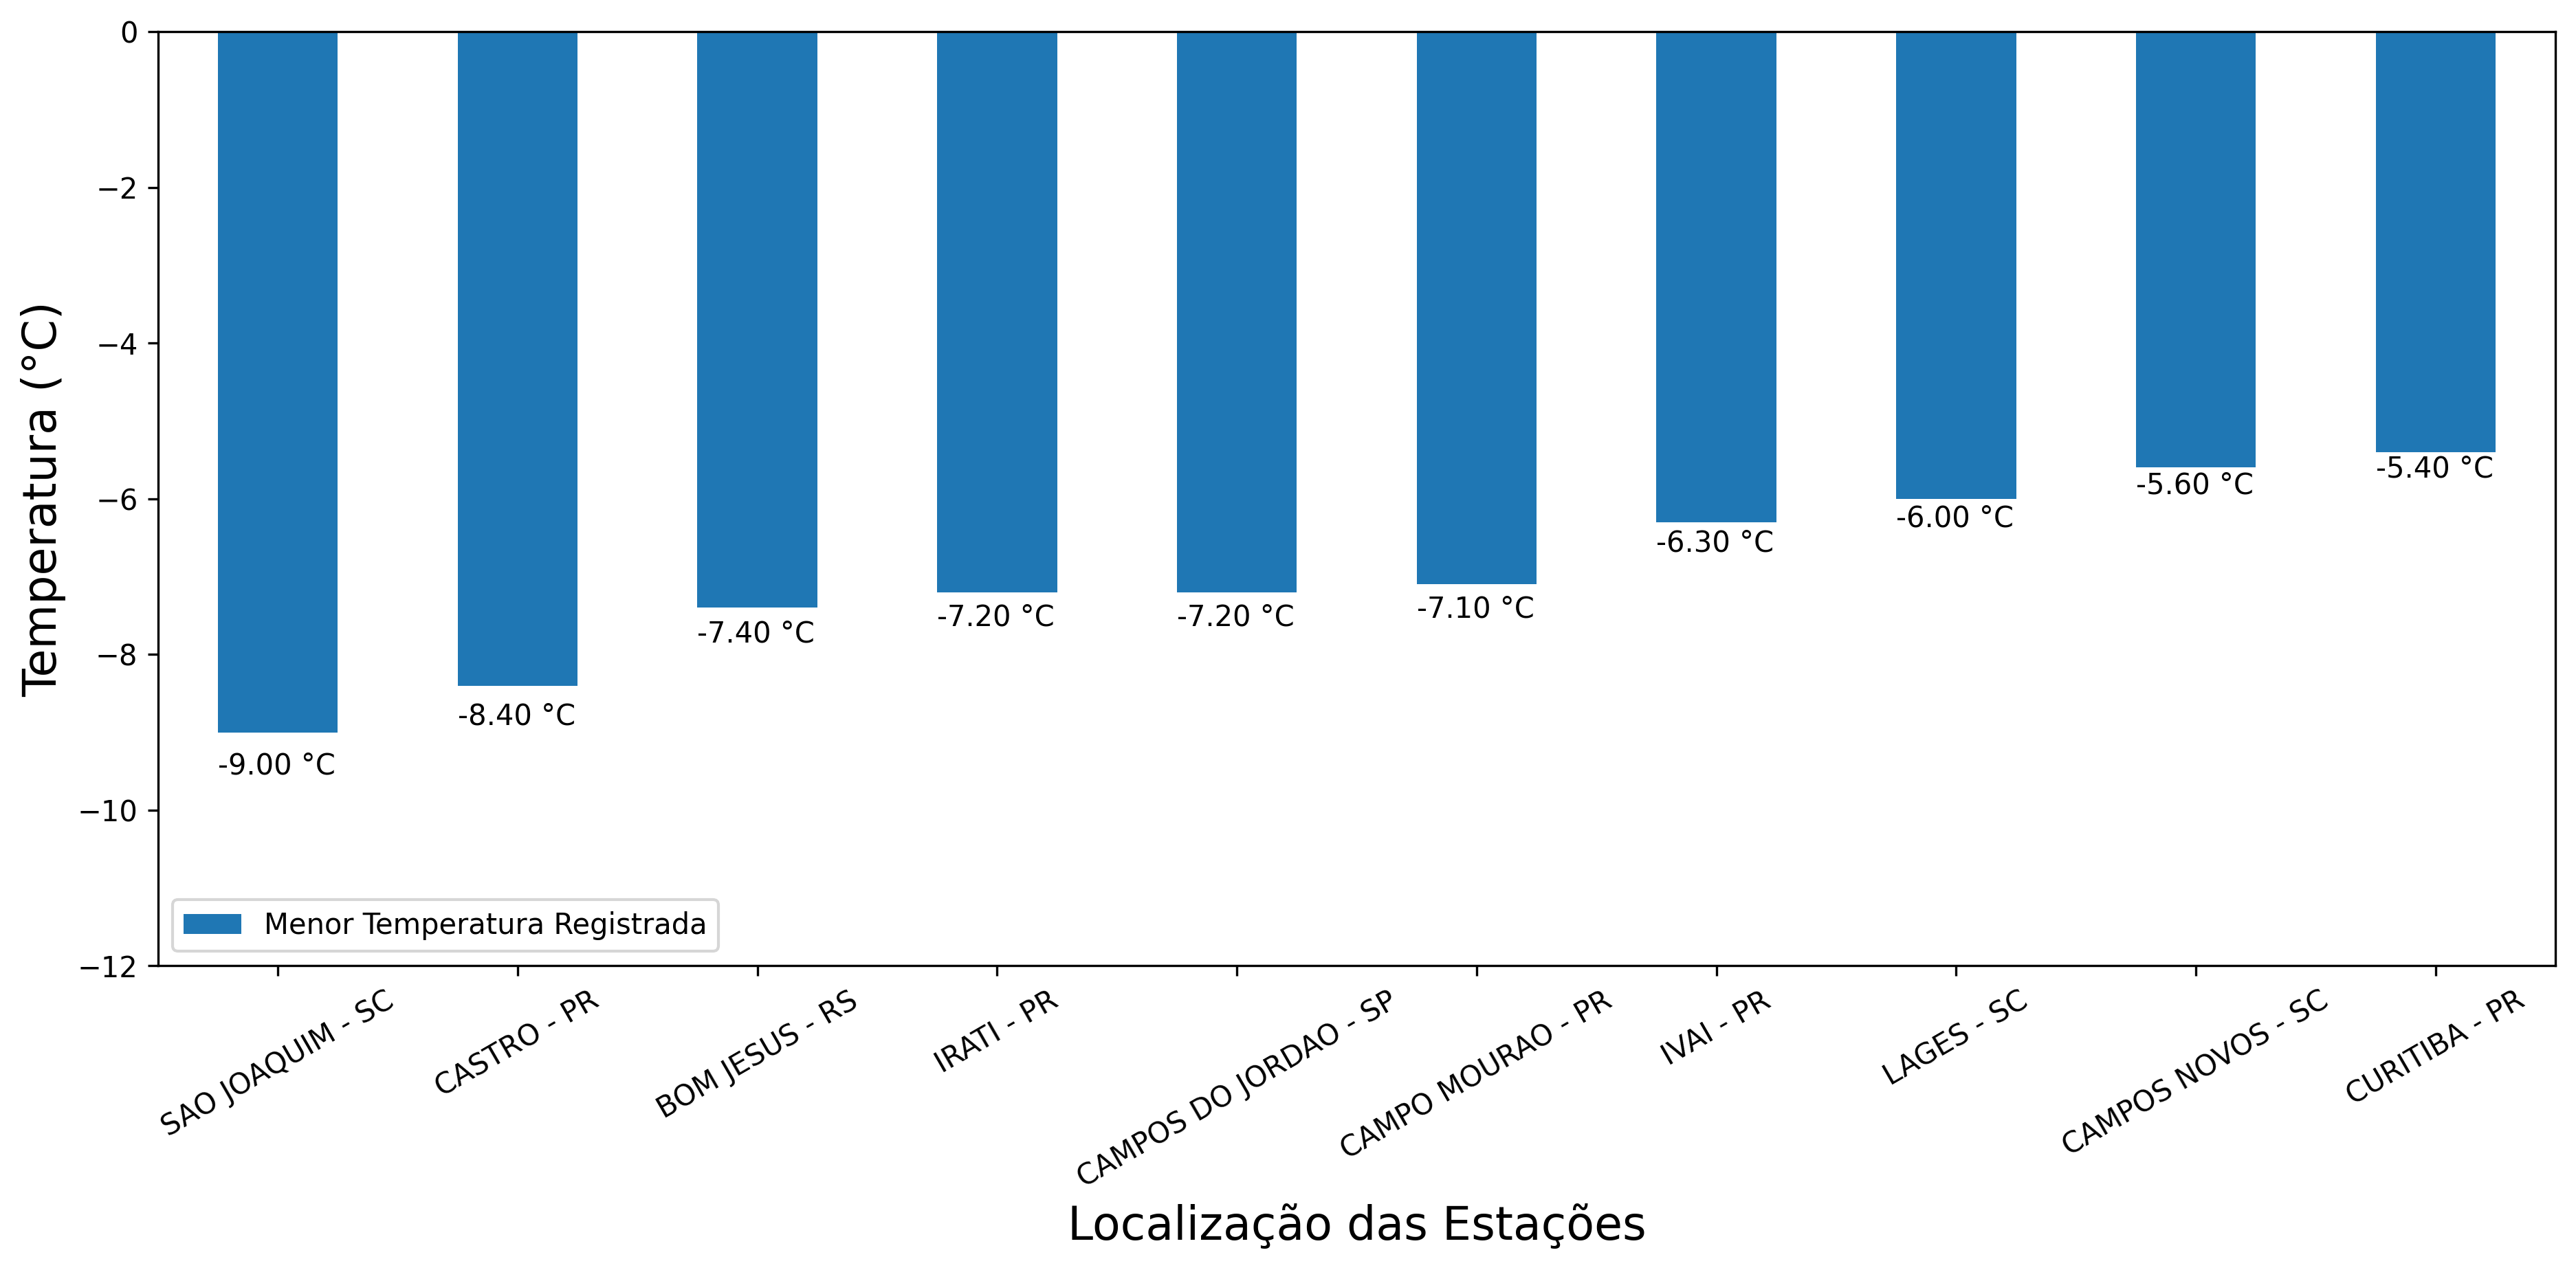
\includegraphics[width=0.9\textwidth]{figuras/estacoes_convencionais_menores_temperaturas.png}
    \label{fig:estacoes_convencionais_menores_temperaturas}
\end{figure}

Realizando uma pesquisa na internet sobre os recordes de temperatura no Brasil encontramos as seguintes informações: 

\begin{displayquote}
"A maior temperatura registrada oficialmente no Brasil foi 44,7 $^{\circ}$C em Bom Jesus, Piauí, em 21 de novembro de 2005, superando o recorde também oficial de Orleans, Santa Catarina, de 44,6 $^{\circ}$C, de 6 de janeiro de 1963. Já a menor temperatura registrada foi de -17,8 $^{\circ}$C no Morro da Igreja, em Urubici, Santa Catarina, em 29 de junho de 1996 (registro extraoficial). A menor temperatura registrada oficialmente no país foi de -14 $^{\circ}$C, no município de Caçador, no mesmo estado, em 11 de junho de 1952." \cite{wiki:clima_do_brasil}.
\end{displayquote}

Essa referência aponta o município de Bom Jesus, no estado do Piauí, com a maior temperatura já registrada no Brasil, com a temperatura alcançando 44,70 $^{\circ}$C em 21 de novembro de 2005, exatamente como os dados das estações convencionais apresentaram.  Também segundo a referência, a menor temperatura já registrada após 1961 foi de -17,8 $^{\circ}$C no Morro da Igreja, em Urubici, Santa Catarina, em 29 de junho de 1996. Analisando os dados, diferente do que apontou a informação encontrada, a menor temperatura registrada pelas estações convencionais foi no município de São Joaquim, em Santa Catarina. Cruzando o mapa de municípios de Santa Catarina com as estações que estamos analisando, observamos que o município de São Joaquim faz fronteira com o município de Urubici e que, dos dois municípios, apenas o de São Joaquim possui, nos dados analisados, estações meteorológicas, o que indica um possível motivo das diferenças entre as informações.

\renewcommand{\cleardoublepage}{}
\renewcommand{\clearpage}{}
\vspace{5mm}
\chapter{Criação dos Modelos de Machine Learning}

Nesta seção, apresentaremos os modelos preditivos desenvolvidos em linguagem Python para a previsão da temperatura para o ano de 2019 utilizando modelos treinados com dados anteriores. Neste trabalho, avaliamos dois modelos preditivos para a previsão da temperatura, o modelo Autoregressive Integrated Moving Average (ARIMA) \cite{whittle1951hypothesis} e um modelo baseado em redes neurais recorrentes utilizando a arquitetura Long Short-Term Memory (LSTM) \cite{hochreiter1997long}.

O modelo ARIMA é um dos modelos lineares mais populares na previsão de séries temporais das últimas décadas, sua popularidade é devido, principalmente, às suas propriedades estatísticas, bem como à conhecida metodologia Box-Jenkins \cite{box2011time} no processo de construção do modelo \cite{zhang2003time}. 

Rede Neural Recorrente (RNN) é um tipo de Rede Neural onde a saída da etapa anterior é alimentada como entrada para a etapa atual, ou seja, ela possui uma “memória” que guarda todas as informações sobre o que foi calculado. A arquitetura de RNN que utilizamos foi a chamada Long Short-Term Memory - LSTM, uma arquitetura de rede neural recorrente específica que foi projetada para modelar sequências temporais e suas dependências de longo alcance com mais precisão do que RNNs convencionais \cite{sak2014long}, características importante quando trabalhamos com longas séries temporais como os dados histórico de temperatura no Brasil. 

Para avaliarmos os modelos que serão desenvolvidos, selecionamos, através de uma amostragem aleatória simples, 10\% das estações convencionais do INMET, 10\% das estações automáticas também do INMET e uma estação automática do LabMet. Após a mostragem, temos um conjunto de amostra de estações que guardam a mesma proporção do conjunto contendo todas as estações. Ao todo, utilizamos 88 estações para avaliar os modelos.  A Tabela \ref{tab:amostra_estacoes} apresenta a quantidade de estações que foram usadas para a avaliação dos modelos de previsão.  

\begin{table}[H]
\caption{Proporção de estações utilizadas para avaliar os modelos desenvolvidos.}
\label{tab:amostra_estacoes}
\begin{adjustbox}{width=\textwidth}
\begin{tabular}{|l|c|r|r|}
\hline
\textbf{Fonte do Dado} & \textbf{Total de Estações} & \textbf{Estações da amostra de avaliação} & \% \\
\hline
Estações Convencionais do INMET  & 265 & 26 & 10\% \\
\hline
Estações Automáticas do INMET & 610 & 61 & 10\% \\
\hline
Estações Automáticas do LabMet & 3 & 1 & 33\% \\
\hline
TOTAL & 878 & 88 & - \\
\hline
\end{tabular}
\end{adjustbox}
\end{table}

\section{Criação do modelo ARIMA}

\subsection{Decomposição das séries temporais}

Uma abstração útil para selecionar métodos de previsão é quebrar uma série temporal em componentes sistemáticos e não sistemáticos. Os componentes sistemáticos podemos considerar que são os que possuem consistência ou recorrência e podem ser descritos e modelados. Já os componentes não sistemáticos são os que não são possíveis de serem modelados \cite{box2011time}.

Pensando nisso, podemos dividir os componentes das séries temporais em:
\begin{itemize}
  \item Nível: o valor médio da série.
  \item Tendência: o valor crescente ou decrescente na série.
  \item Sazonalidade: o ciclo repetitivo de curto prazo na série.
  \item Ruído: a variação aleatória da série.
\end{itemize}

Para esta analise, iremos apresentar apenas os resultados para três estações de exemplo que foram escolhidas a partir das estações de avaliação.

Decompondo as séries temporais das estações de exemplo, obtivemos os resultados apresentados nas figuras \ref{fig:decomposicao_1}, \ref{fig:decomposicao_2} e \ref{fig:decomposicao_3}.

\begin{figure}[H]
    \centering
    \caption{Decomposição da série temporal da temperatura do ar para a estação convencional localizada no município de Balsas, no estado do Maranhão.}
    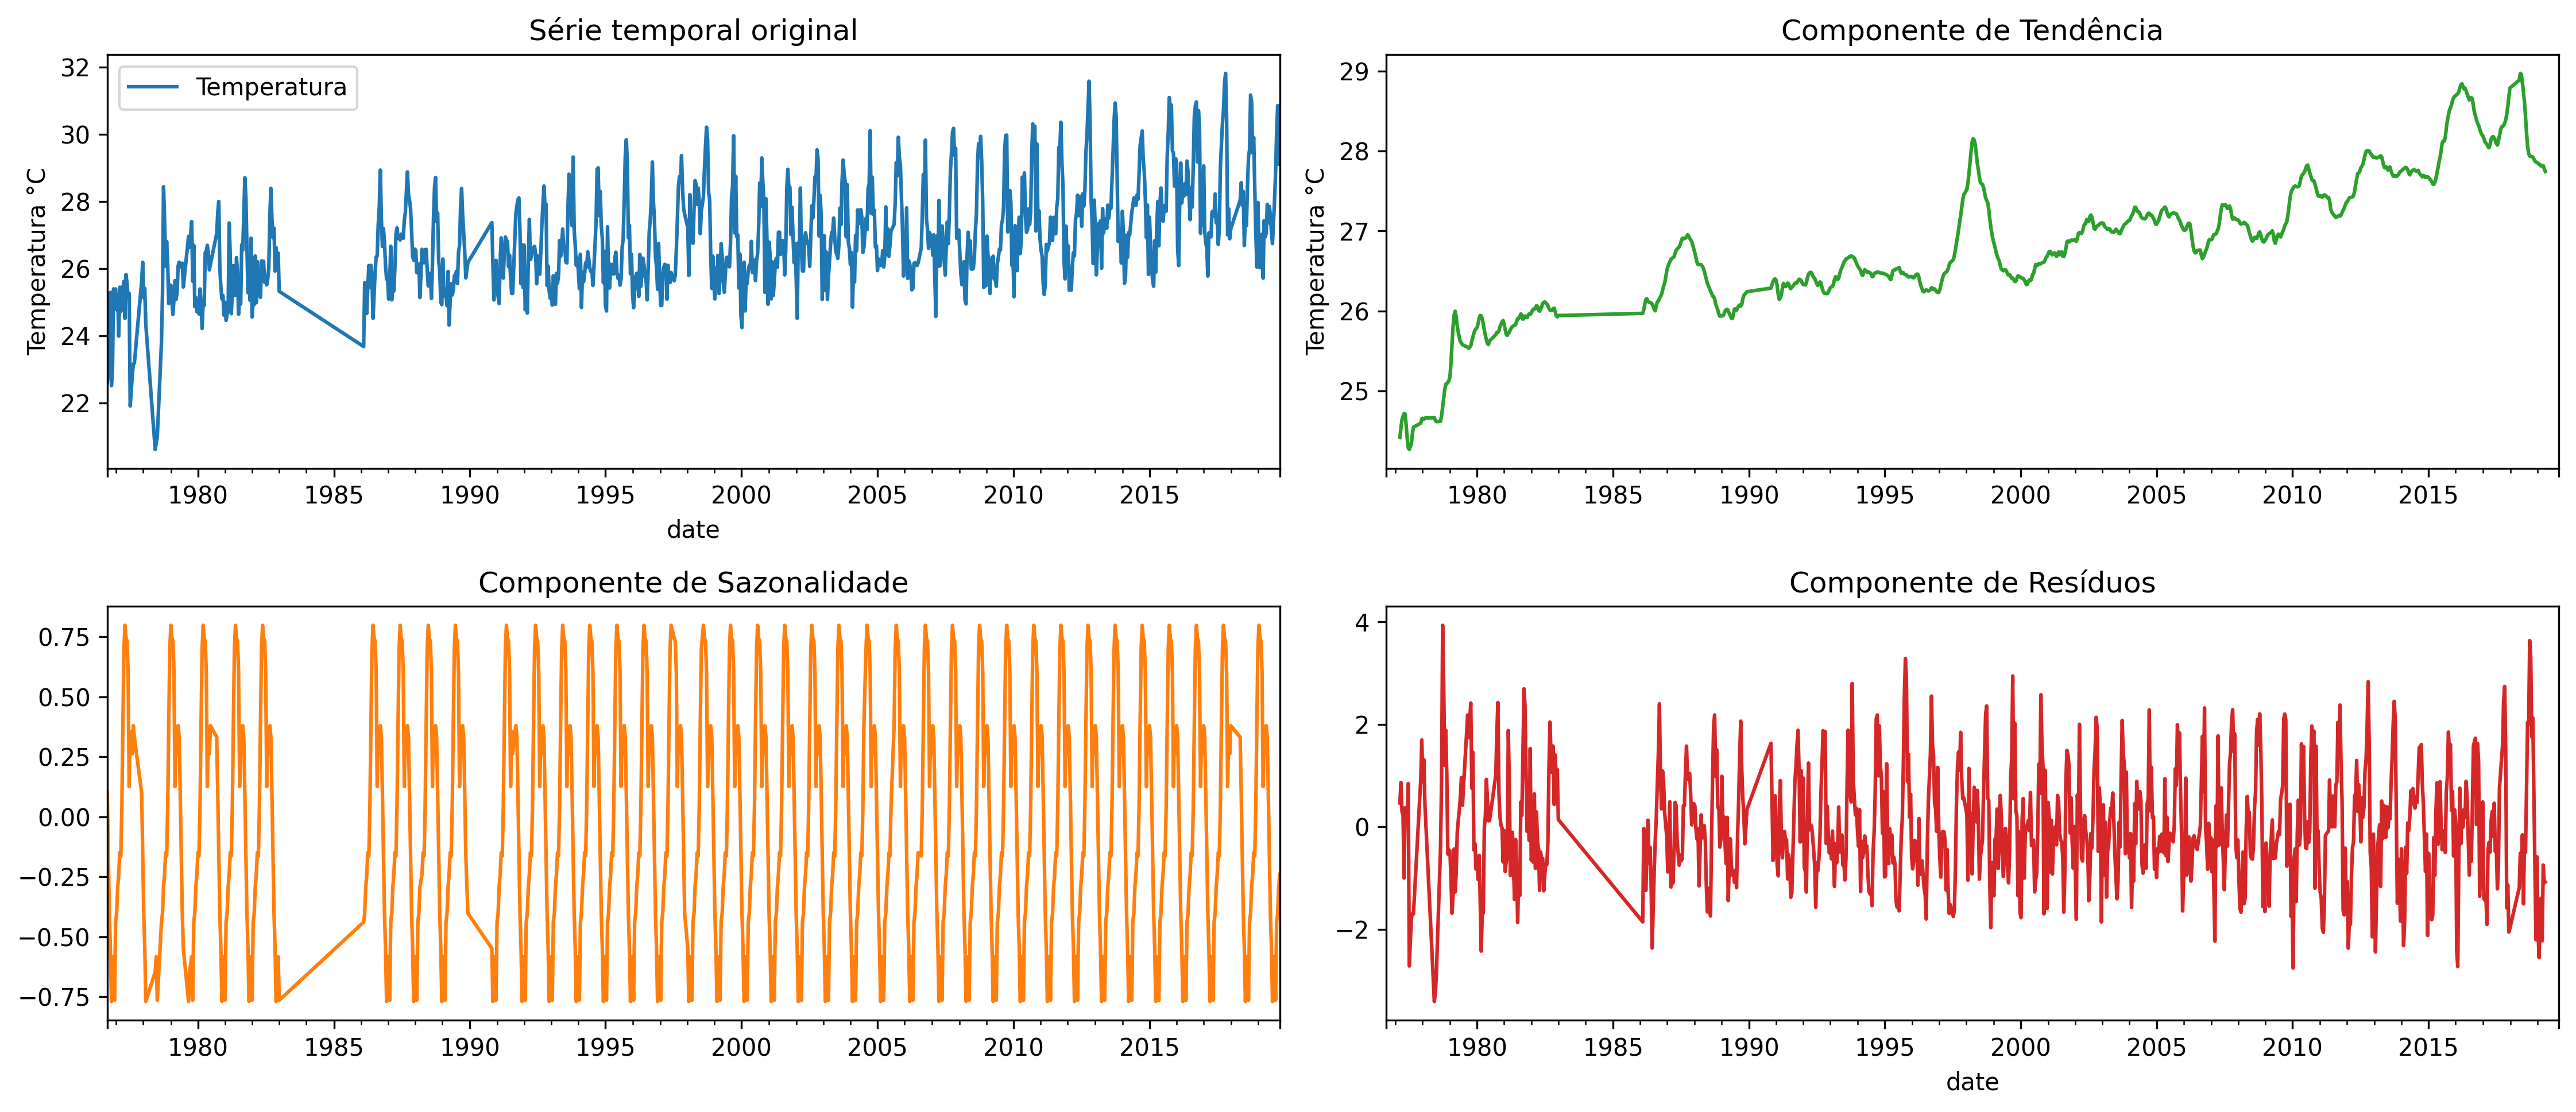
\includegraphics[width=0.9\textwidth]{figuras/decomposicao_82768.png}
    \label{fig:decomposicao_1}
\end{figure}

\begin{figure}[H]
    \centering
    \caption{Decomposição da série temporal da temperatura do ar para a estação automática localizada no município de Ariranha, no estado de São Paulo.}
    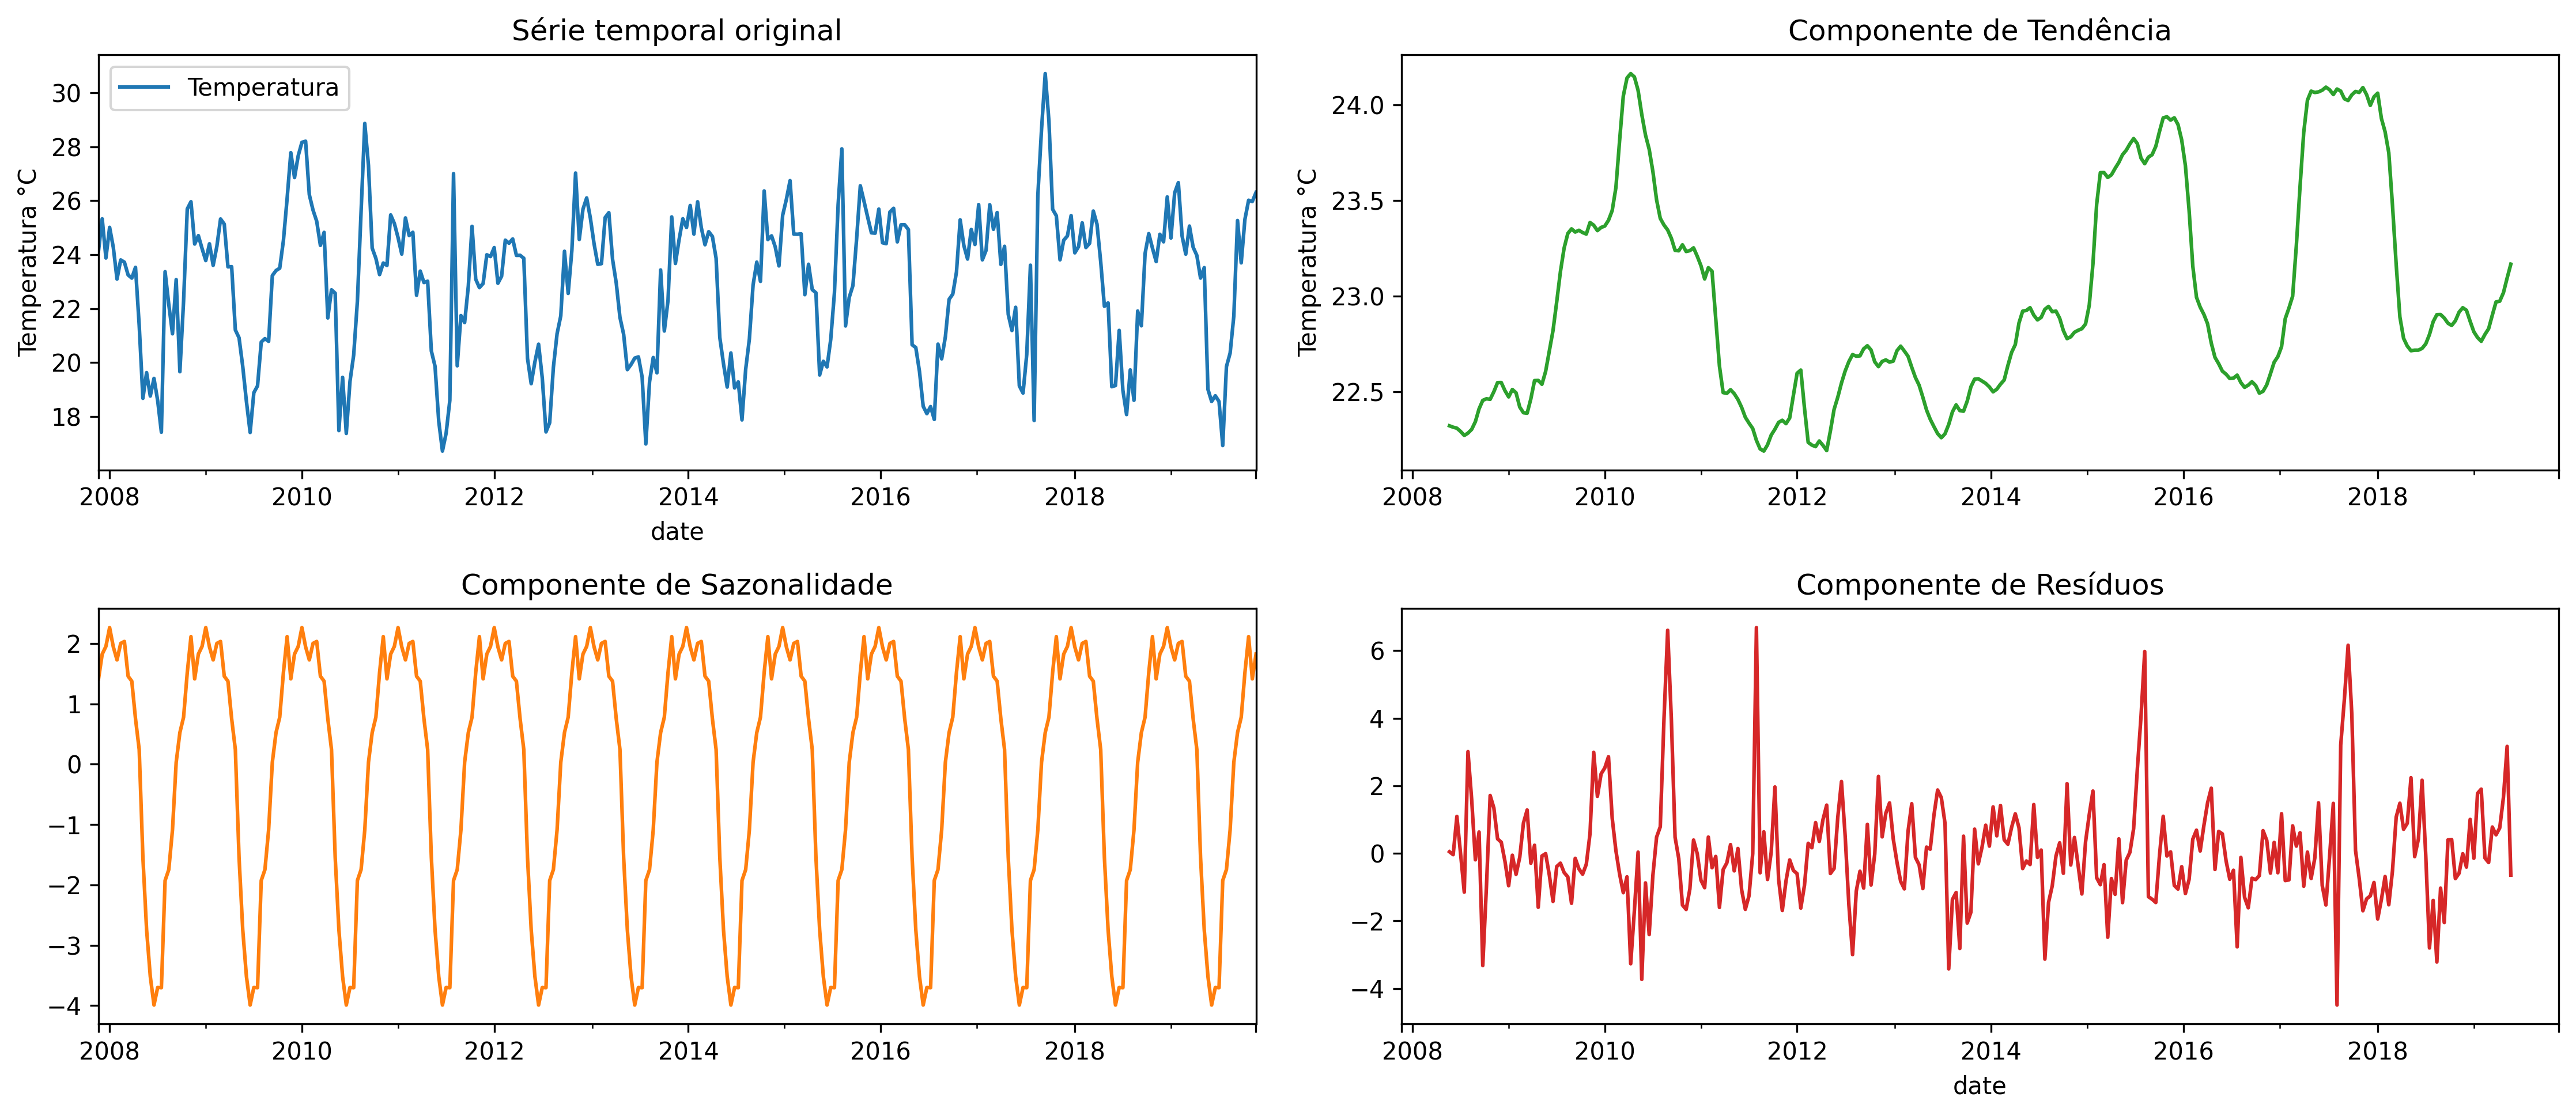
\includegraphics[width=0.9\textwidth]{figuras/decomposicao_A736.png}
    \label{fig:decomposicao_2}
\end{figure}

\begin{figure}[H]
    \centering
    \caption{Decomposição da série temporal da temperatura do ar para a estação automática localizada no município de Petrolina, no estado de Pernambuco.}
    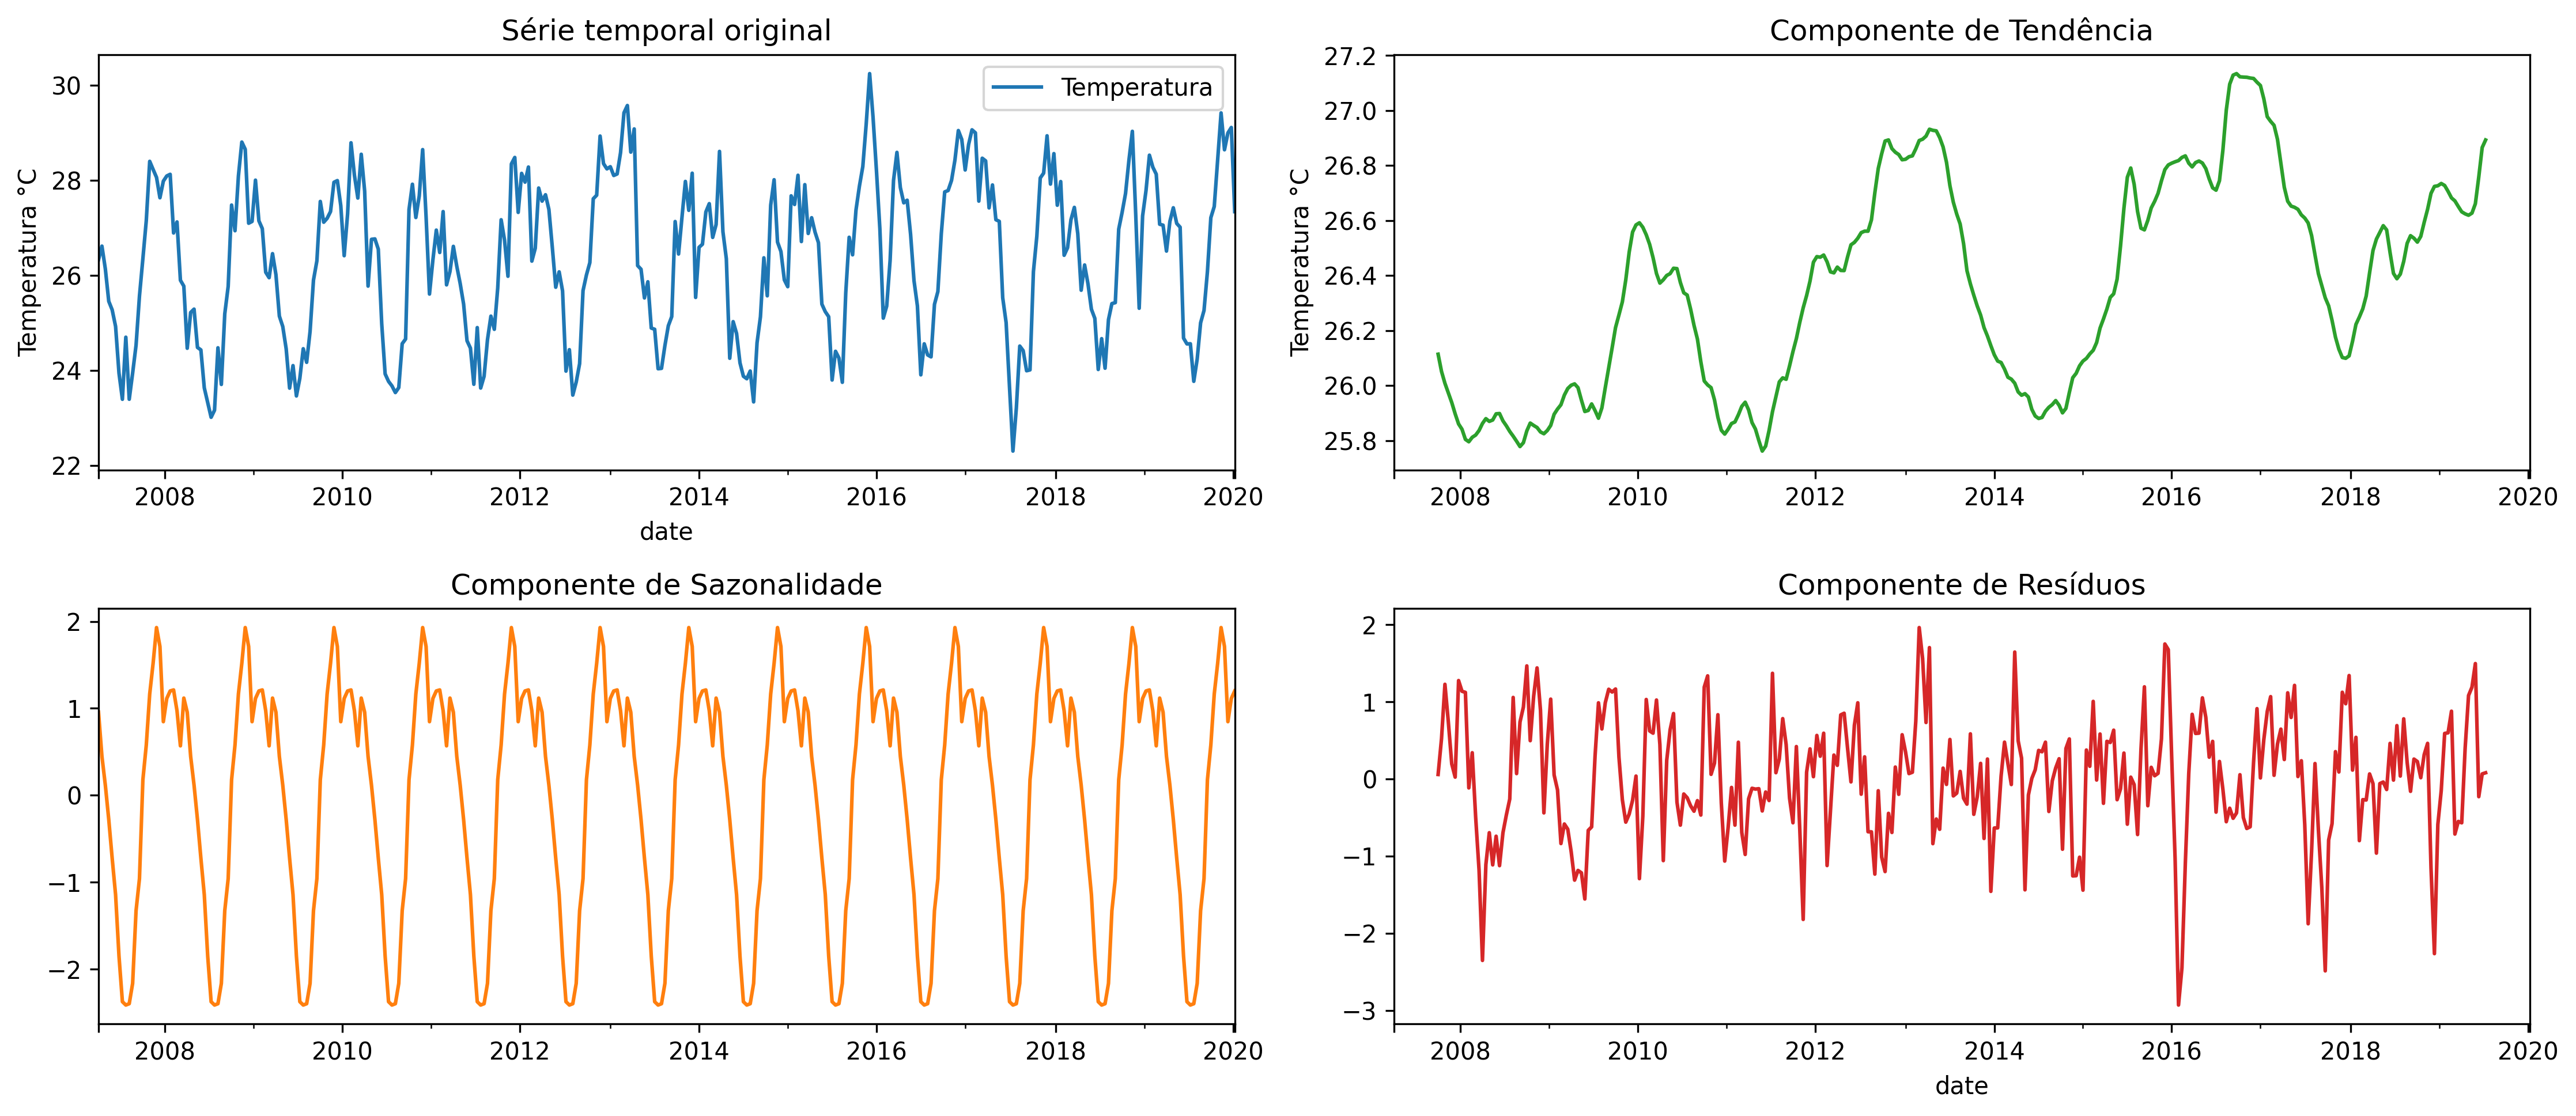
\includegraphics[width=0.9\textwidth]{figuras/decomposicao_712f3e11658051636f09732a60fb3c1b.png}
    \label{fig:decomposicao_3}
\end{figure}

Observando os componentes das séries temporais de exemplo, é possível observarmos uma forte tendencia anual nos dados de temperatura, confirmando a hipótese de que essa variável possui essa característica em seu comportamento.

\subsection{Autocorrelação das séries temporais}

Ao plotarmos a Autocorrelação para essas mesmas estações de exemplo, temos as figuras \ref{fig:correlacao_1}, \ref{fig:correlacao_2} e \ref{fig:correlacao_3}. 

\begin{figure}[H]
    \centering
    \caption{Autocorrelação da série temporal da temperatura do ar para a estação convencional localizada no município de Balsas, no estado do Maranhão.}
    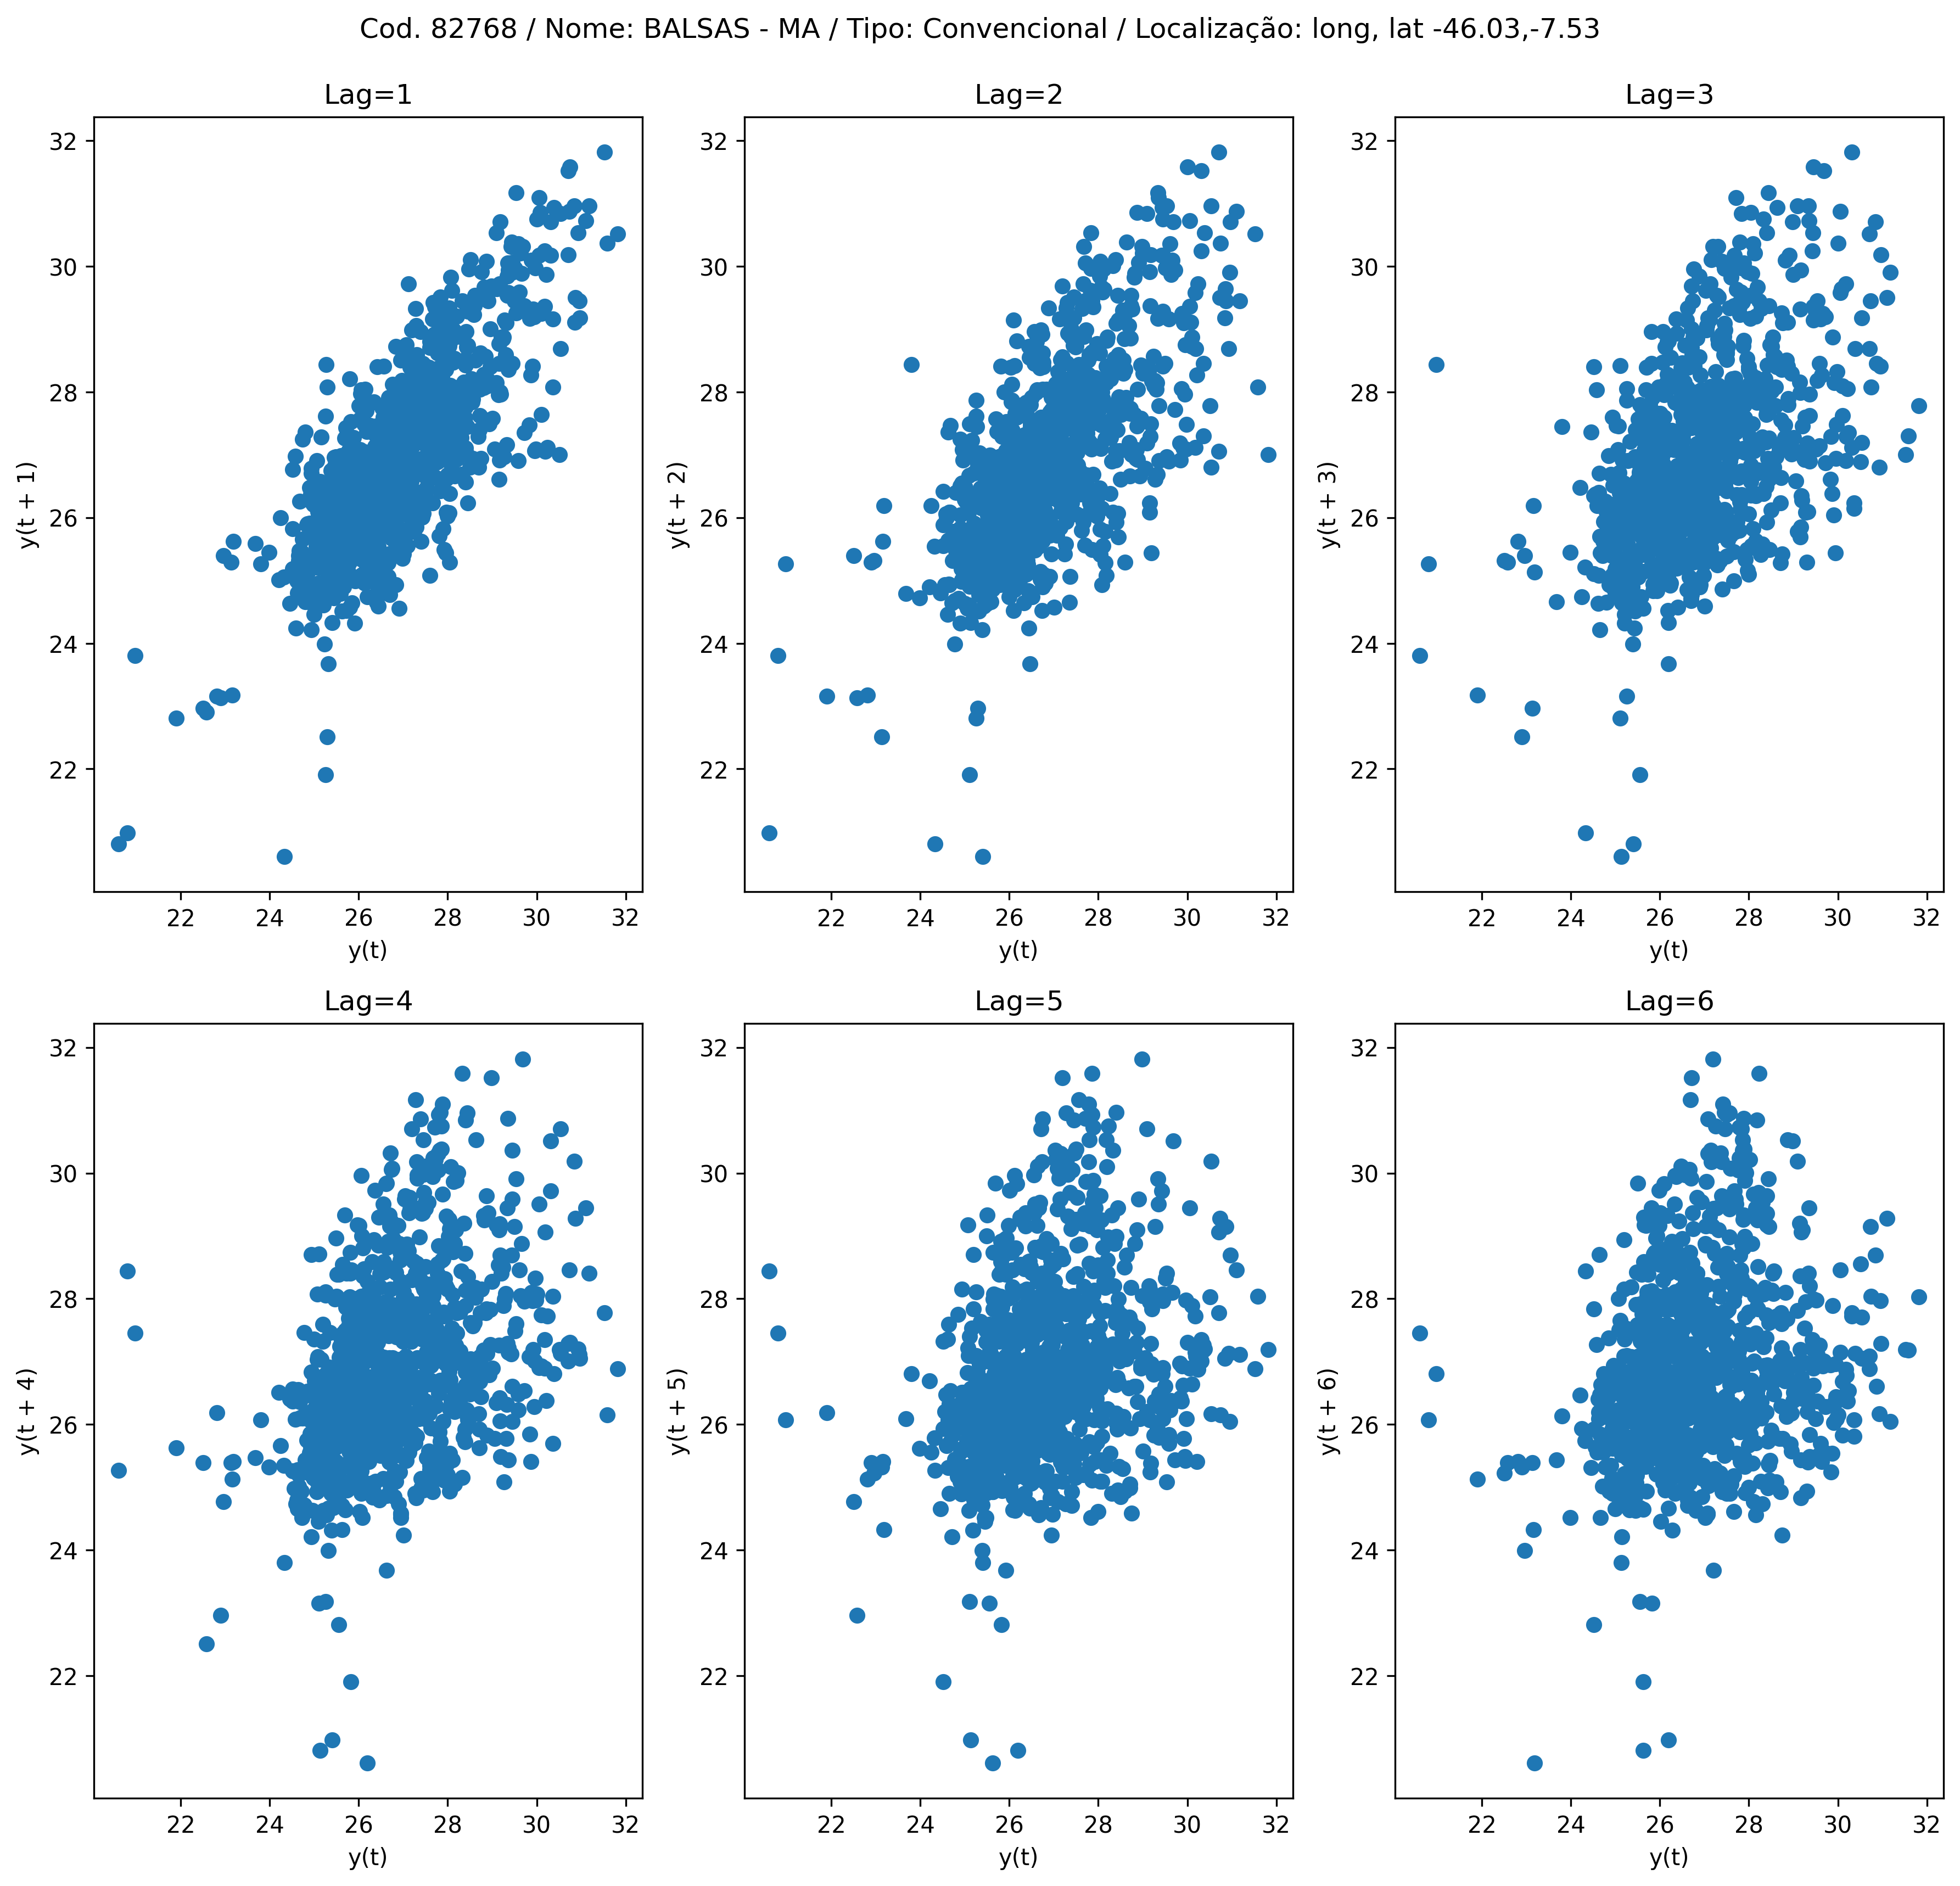
\includegraphics[width=0.9\textwidth]{figuras/correlacao_82768.png}
    \label{fig:correlacao_1}
\end{figure}

\begin{figure}[H]
    \centering
    \caption{Autocorrelação da série temporal da temperatura do ar para a estação automática localizada no município de Ariranha, no estado de São Paulo.}
    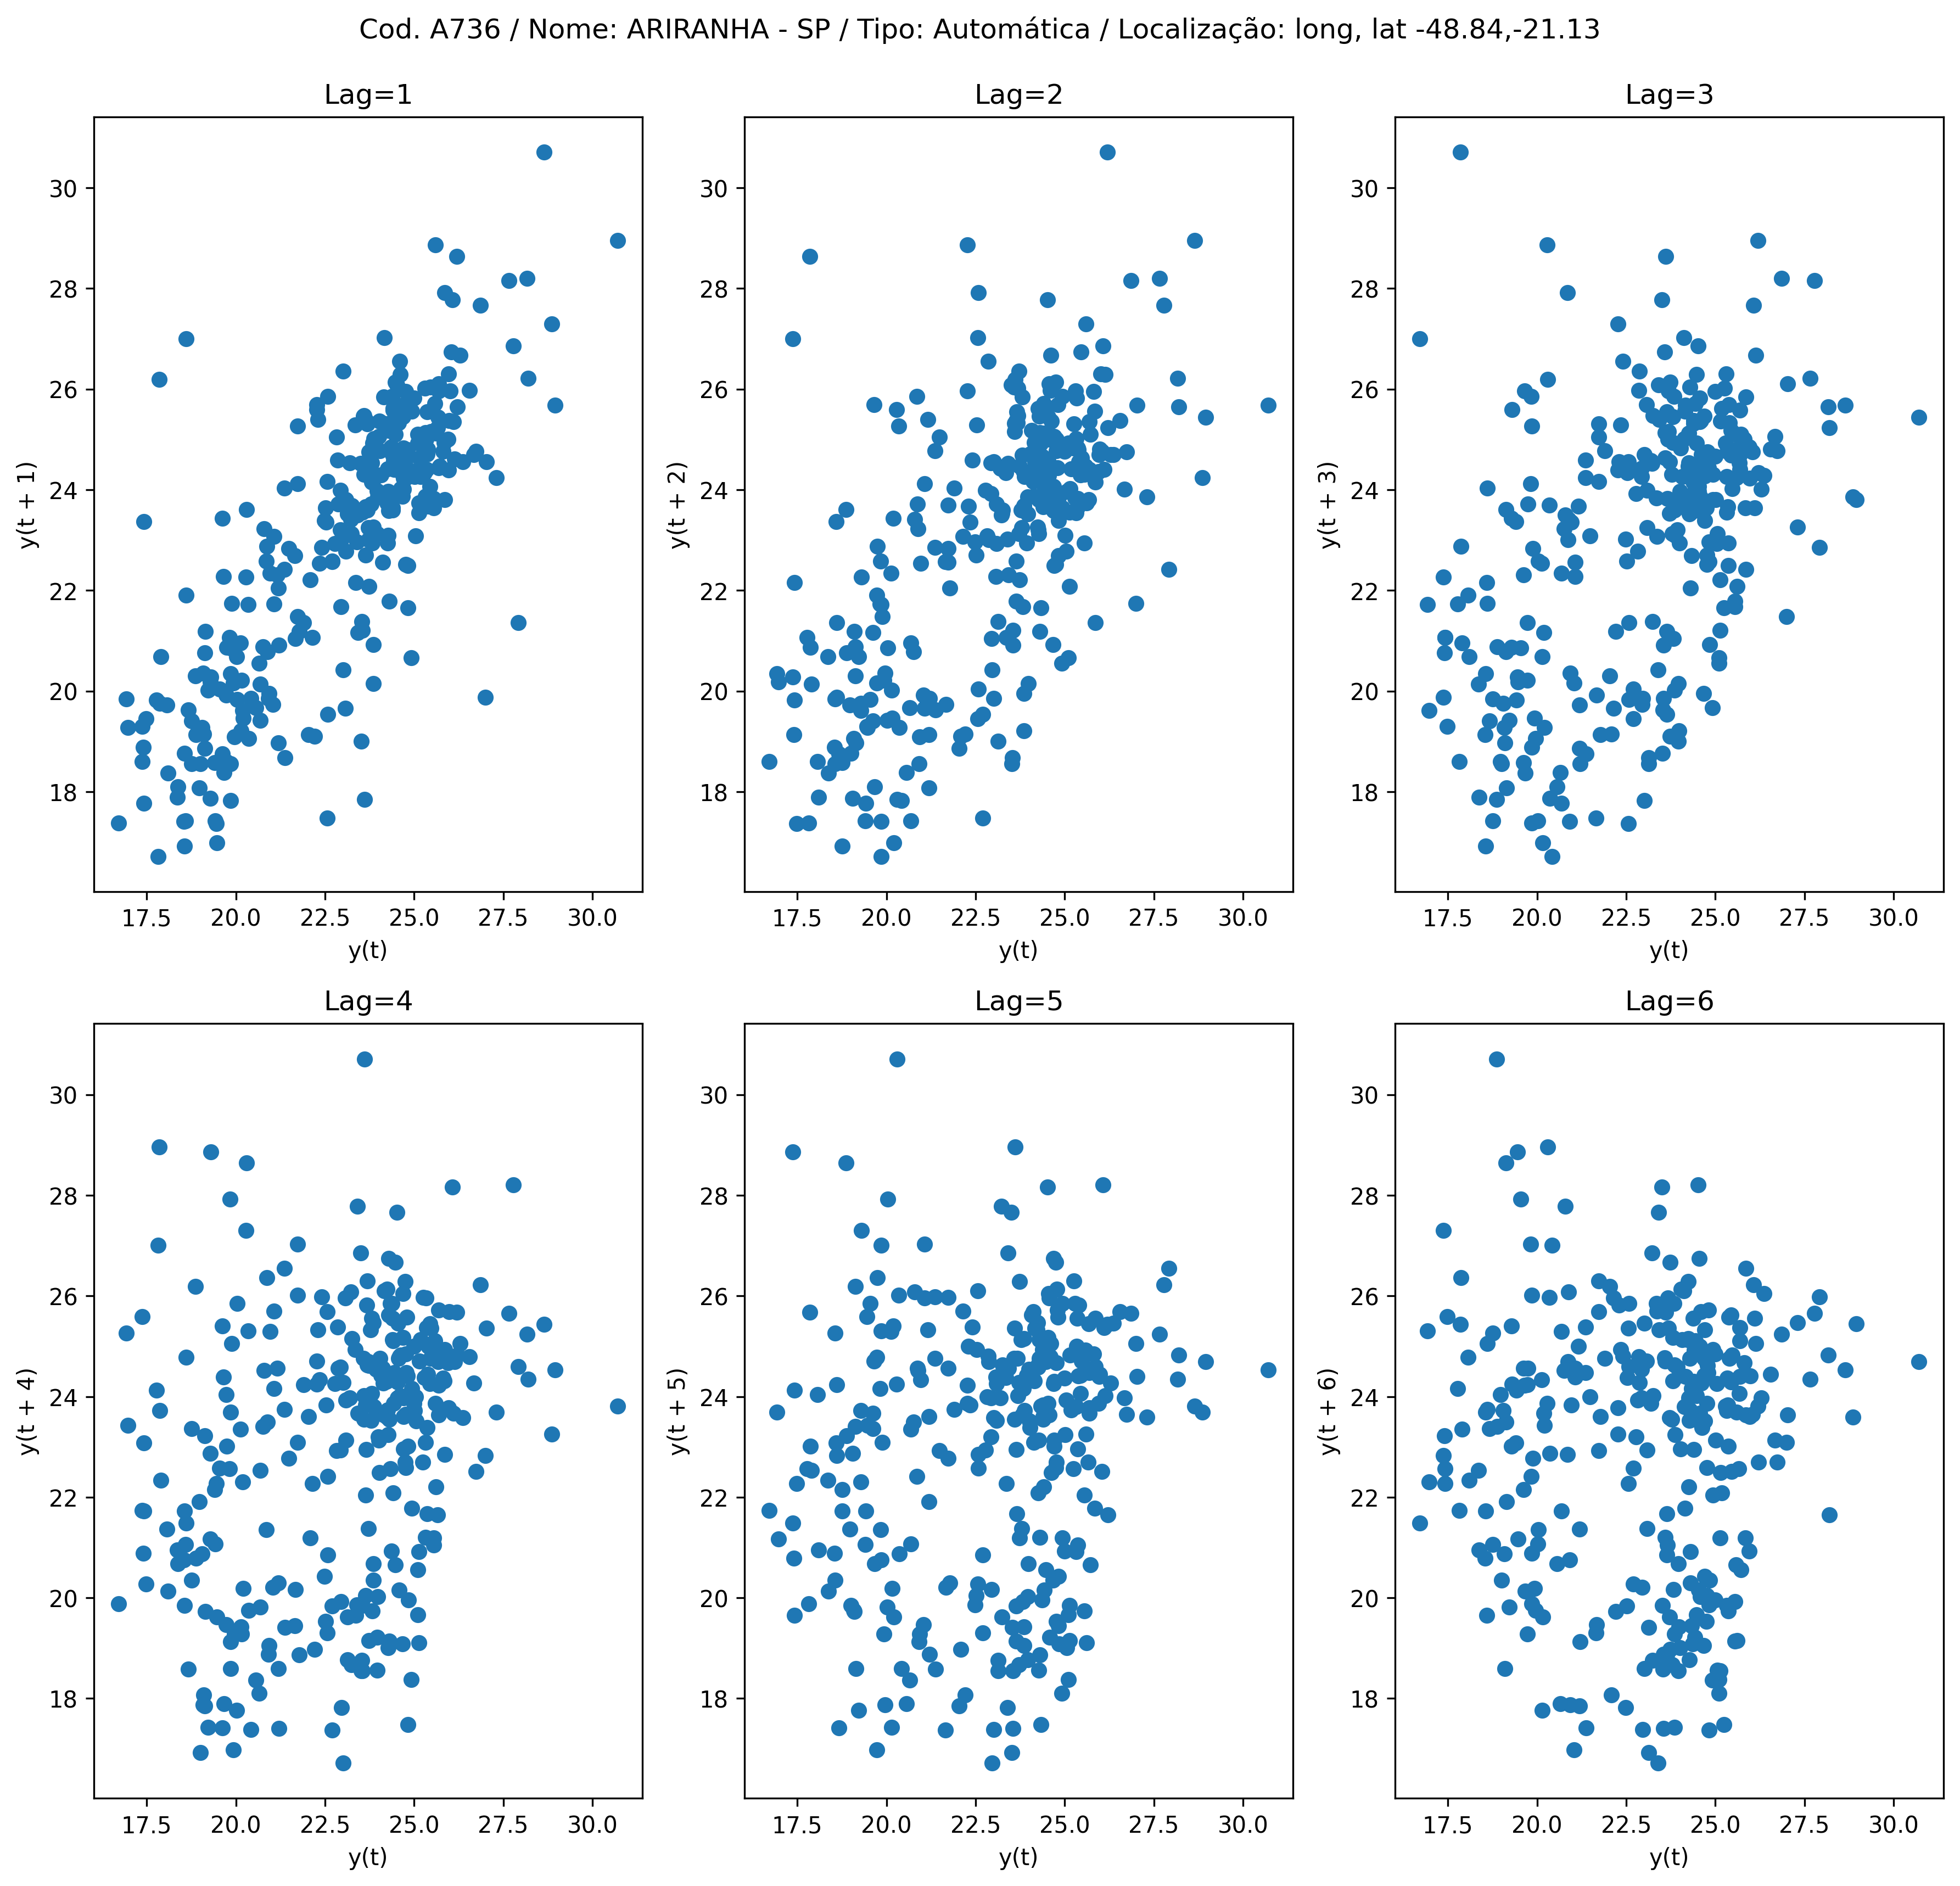
\includegraphics[width=0.9\textwidth]{figuras/correlacao_A736.png}
    \label{fig:correlacao_2}
\end{figure}

\begin{figure}[H]
    \centering
    \caption{Autocorrelação da série temporal da temperatura do ar para a estação automática localizada no município de Petrolina, no estado de Pernambuco.}
    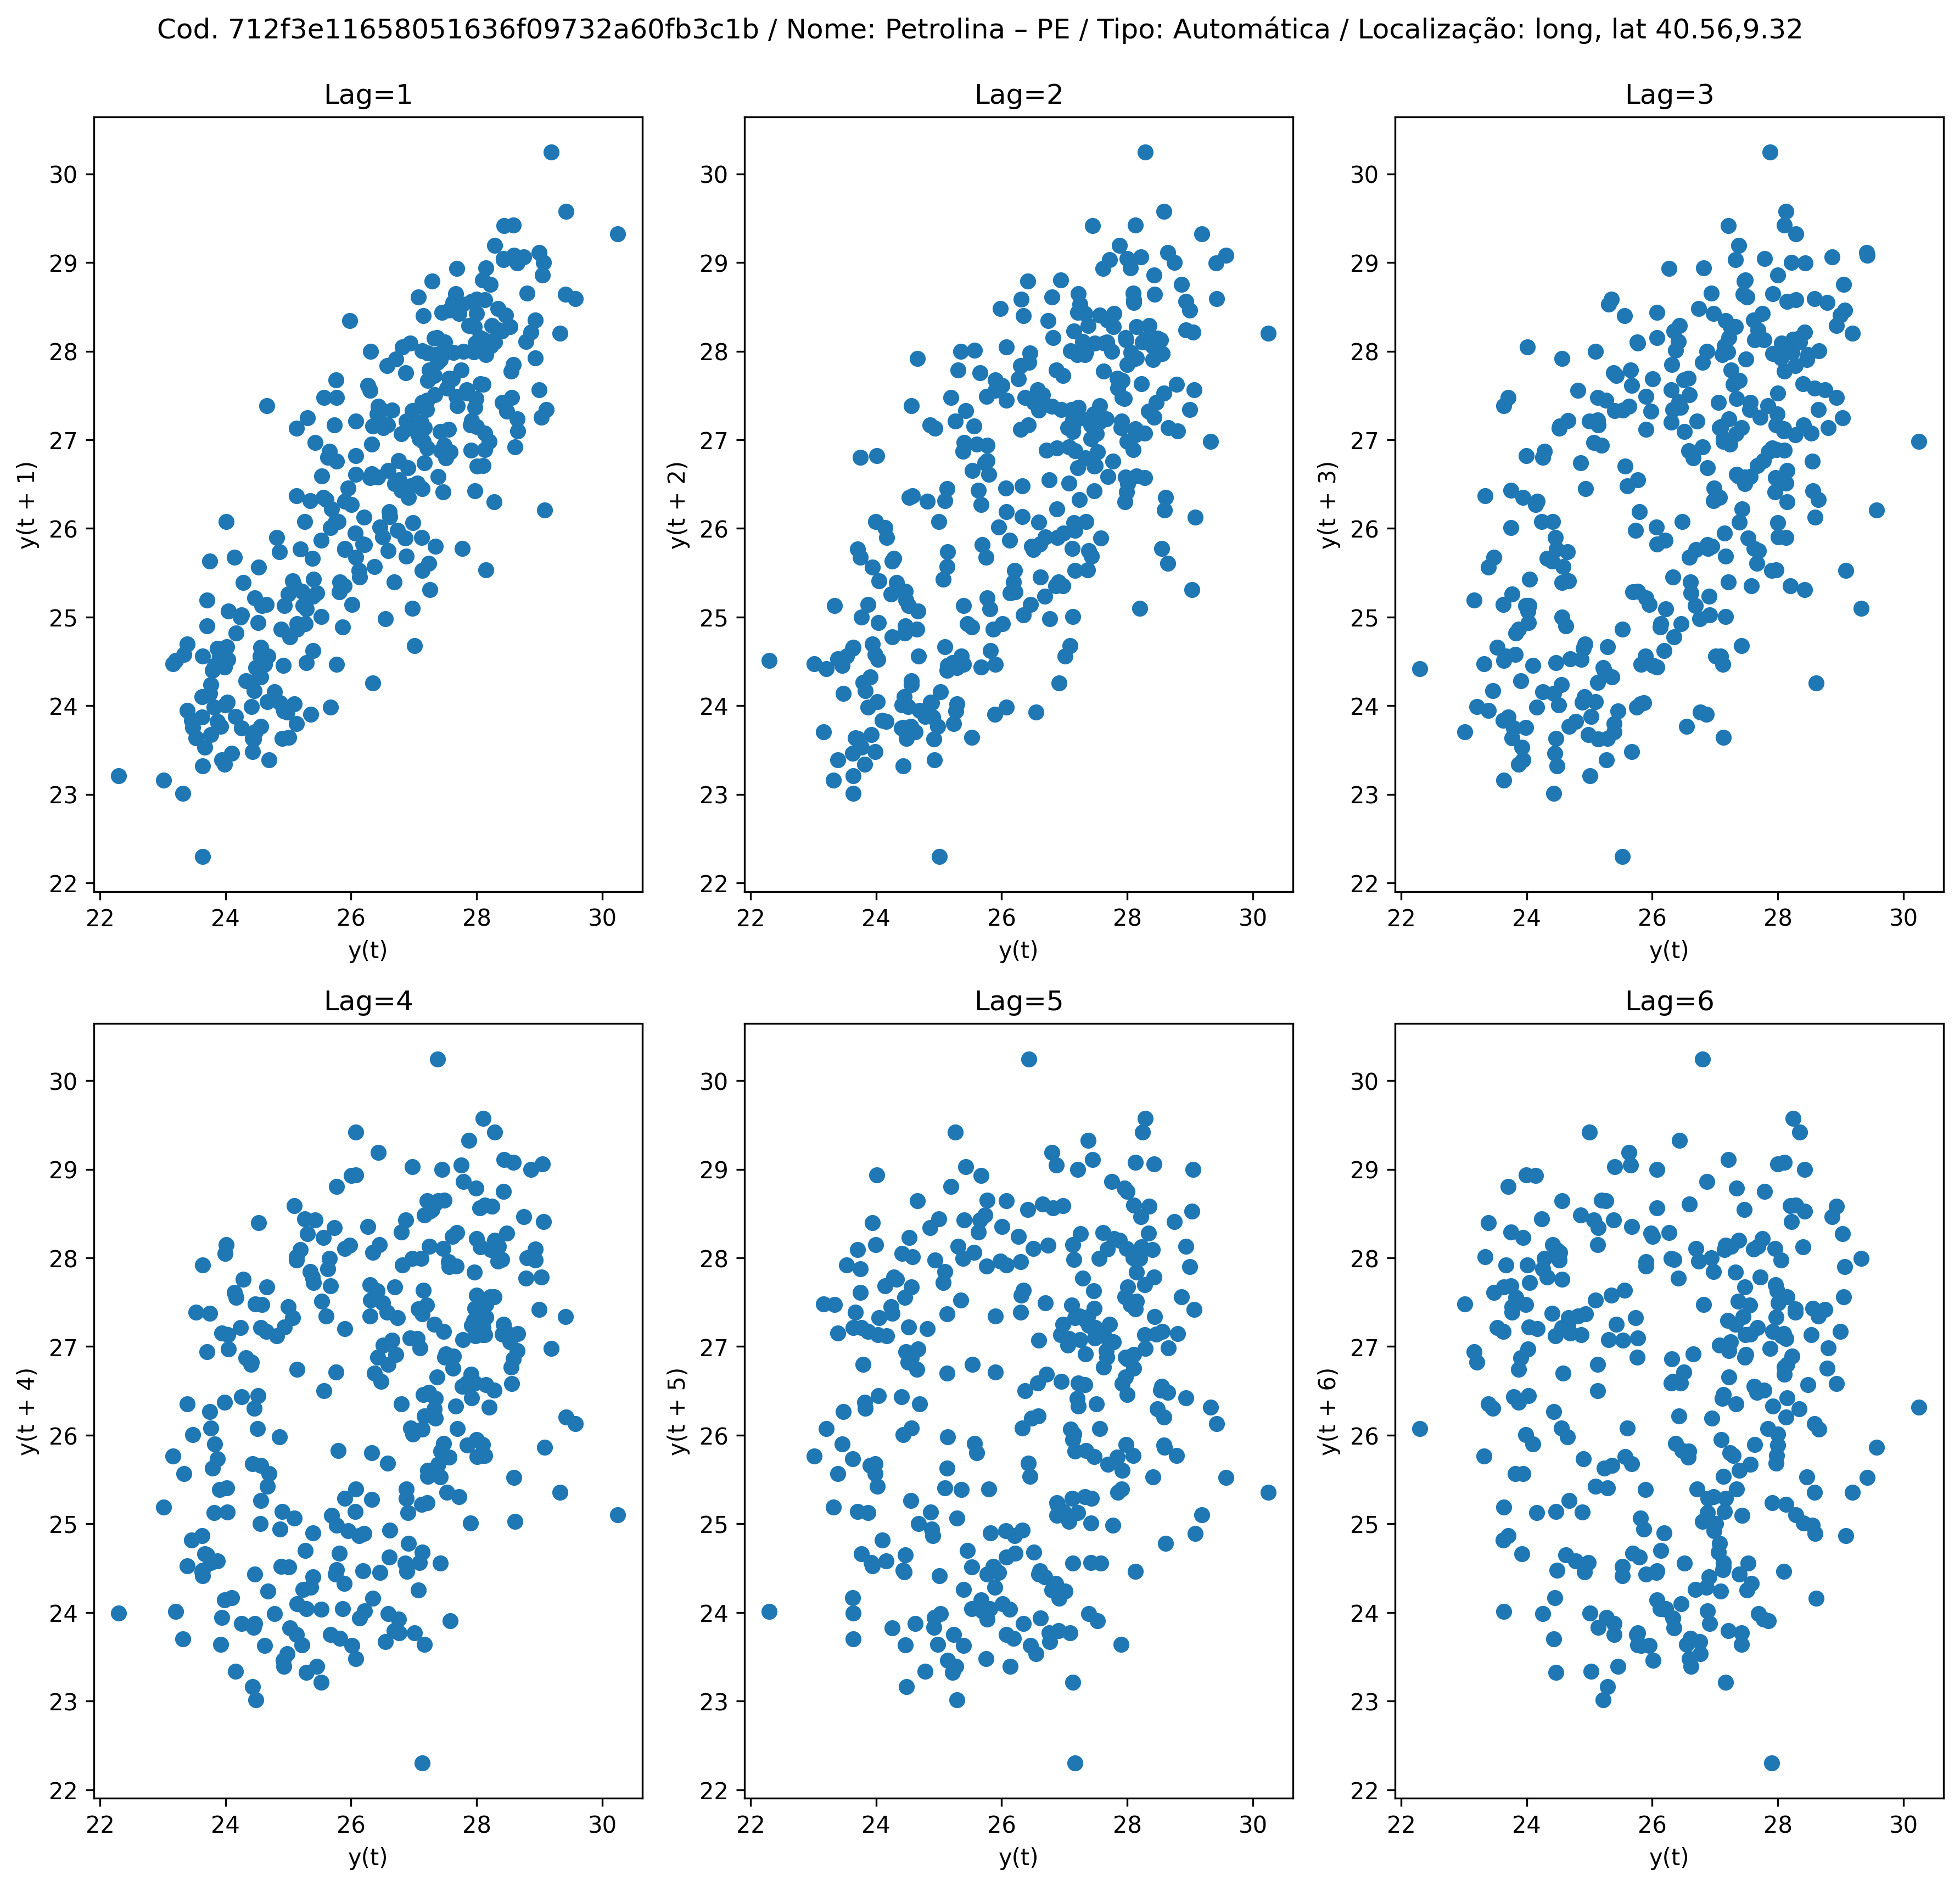
\includegraphics[width=0.9\textwidth]{figuras/correlacao_712f3e11658051636f09732a60fb3c1b.png}
    \label{fig:correlacao_3}
\end{figure}

Verificando os gráficos de autocorrelação, podemos verificar que não há uma alta autocorrelação nas estações de exemplo, por isso há a necessidade de se utilizar um modelo auto-arima para identificação do melhor modelo de forma automática.

\subsection{Verificando a estacionalidade}

A maioria dos modelos de previsão de séries temporais exigem que os dados sejam estacionários. Uma série temporal é considerada estacionária se suas propriedades estatísticas, como média, variância e covariância permanecerem constantes ao longo do tempo \cite{box2011time}. Para verificarmos se as séries que estamos trabalhando são estacionárias, utilizamos o teste de Dickey-Fuller aumentado \cite{said1984testing}. 

Apresentamos o resultado da verificação da estacionalidade das estações utilizadas como exemplo nas Figuras \ref{fig:estacionalidade_seria_original_1}, \ref{fig:estacionalidade_seria_original_2} e \ref{fig:estacionalidade_seria_original_3}.

\begin{figure}[H]
    \centering
    \caption{Teste de estacionalidade da série temporal da temperatura do ar para a estação convencional localizada no município de Balsas, no estado do Maranhão.}
    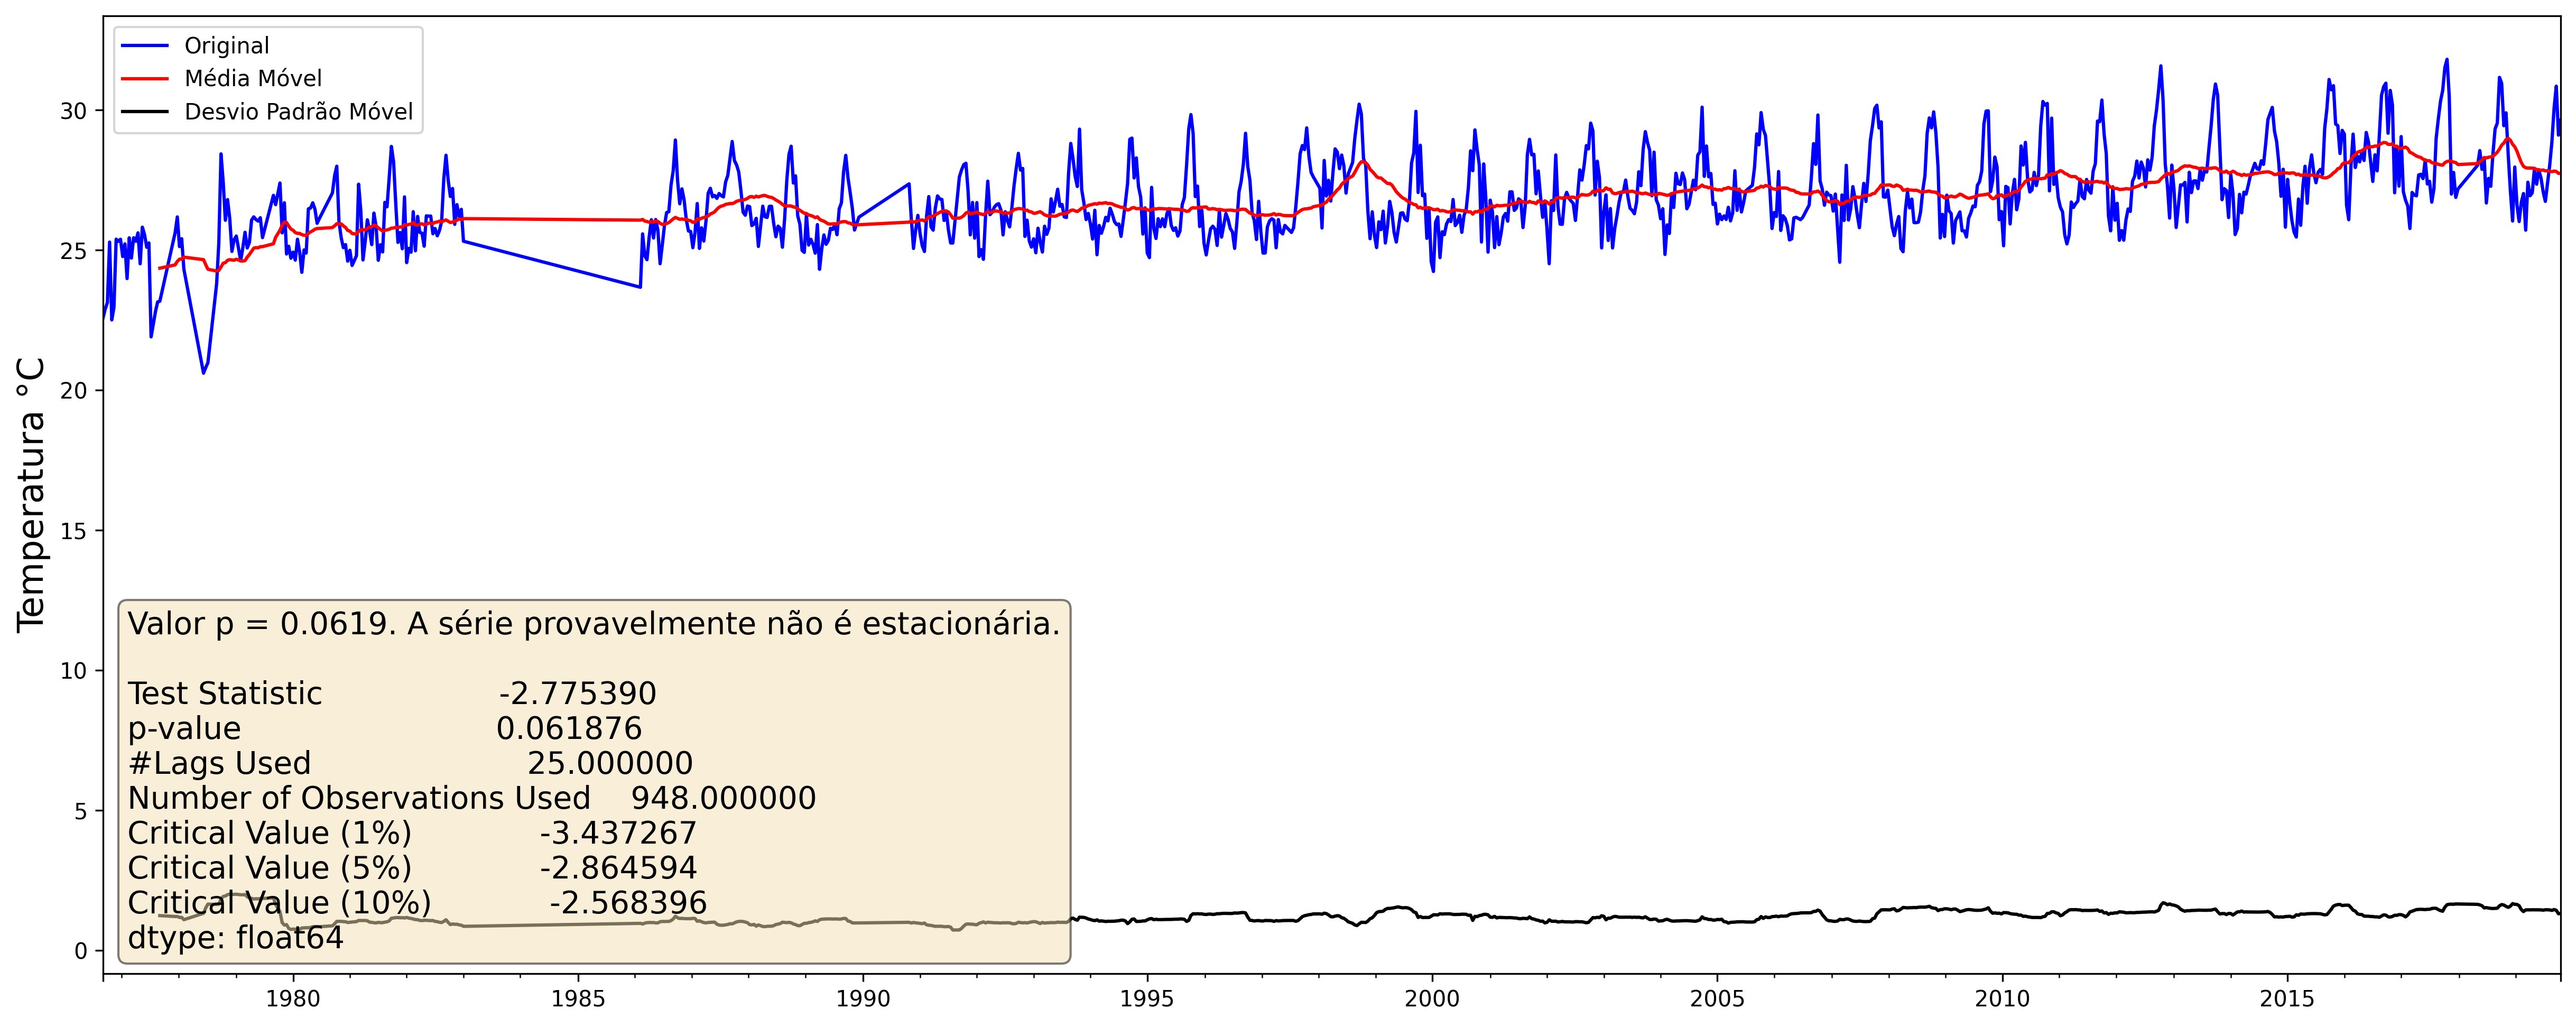
\includegraphics[width=0.9\textwidth]{figuras/dickey_fuller_raw_82768.png}
    \label{fig:estacionalidade_seria_original_1}
\end{figure}

\begin{figure}[H]
    \centering
    \caption{Teste de estacionalidade da série temporal da temperatura do ar para a estação automática localizada no município de Ariranha, no estado de São Paulo.}
    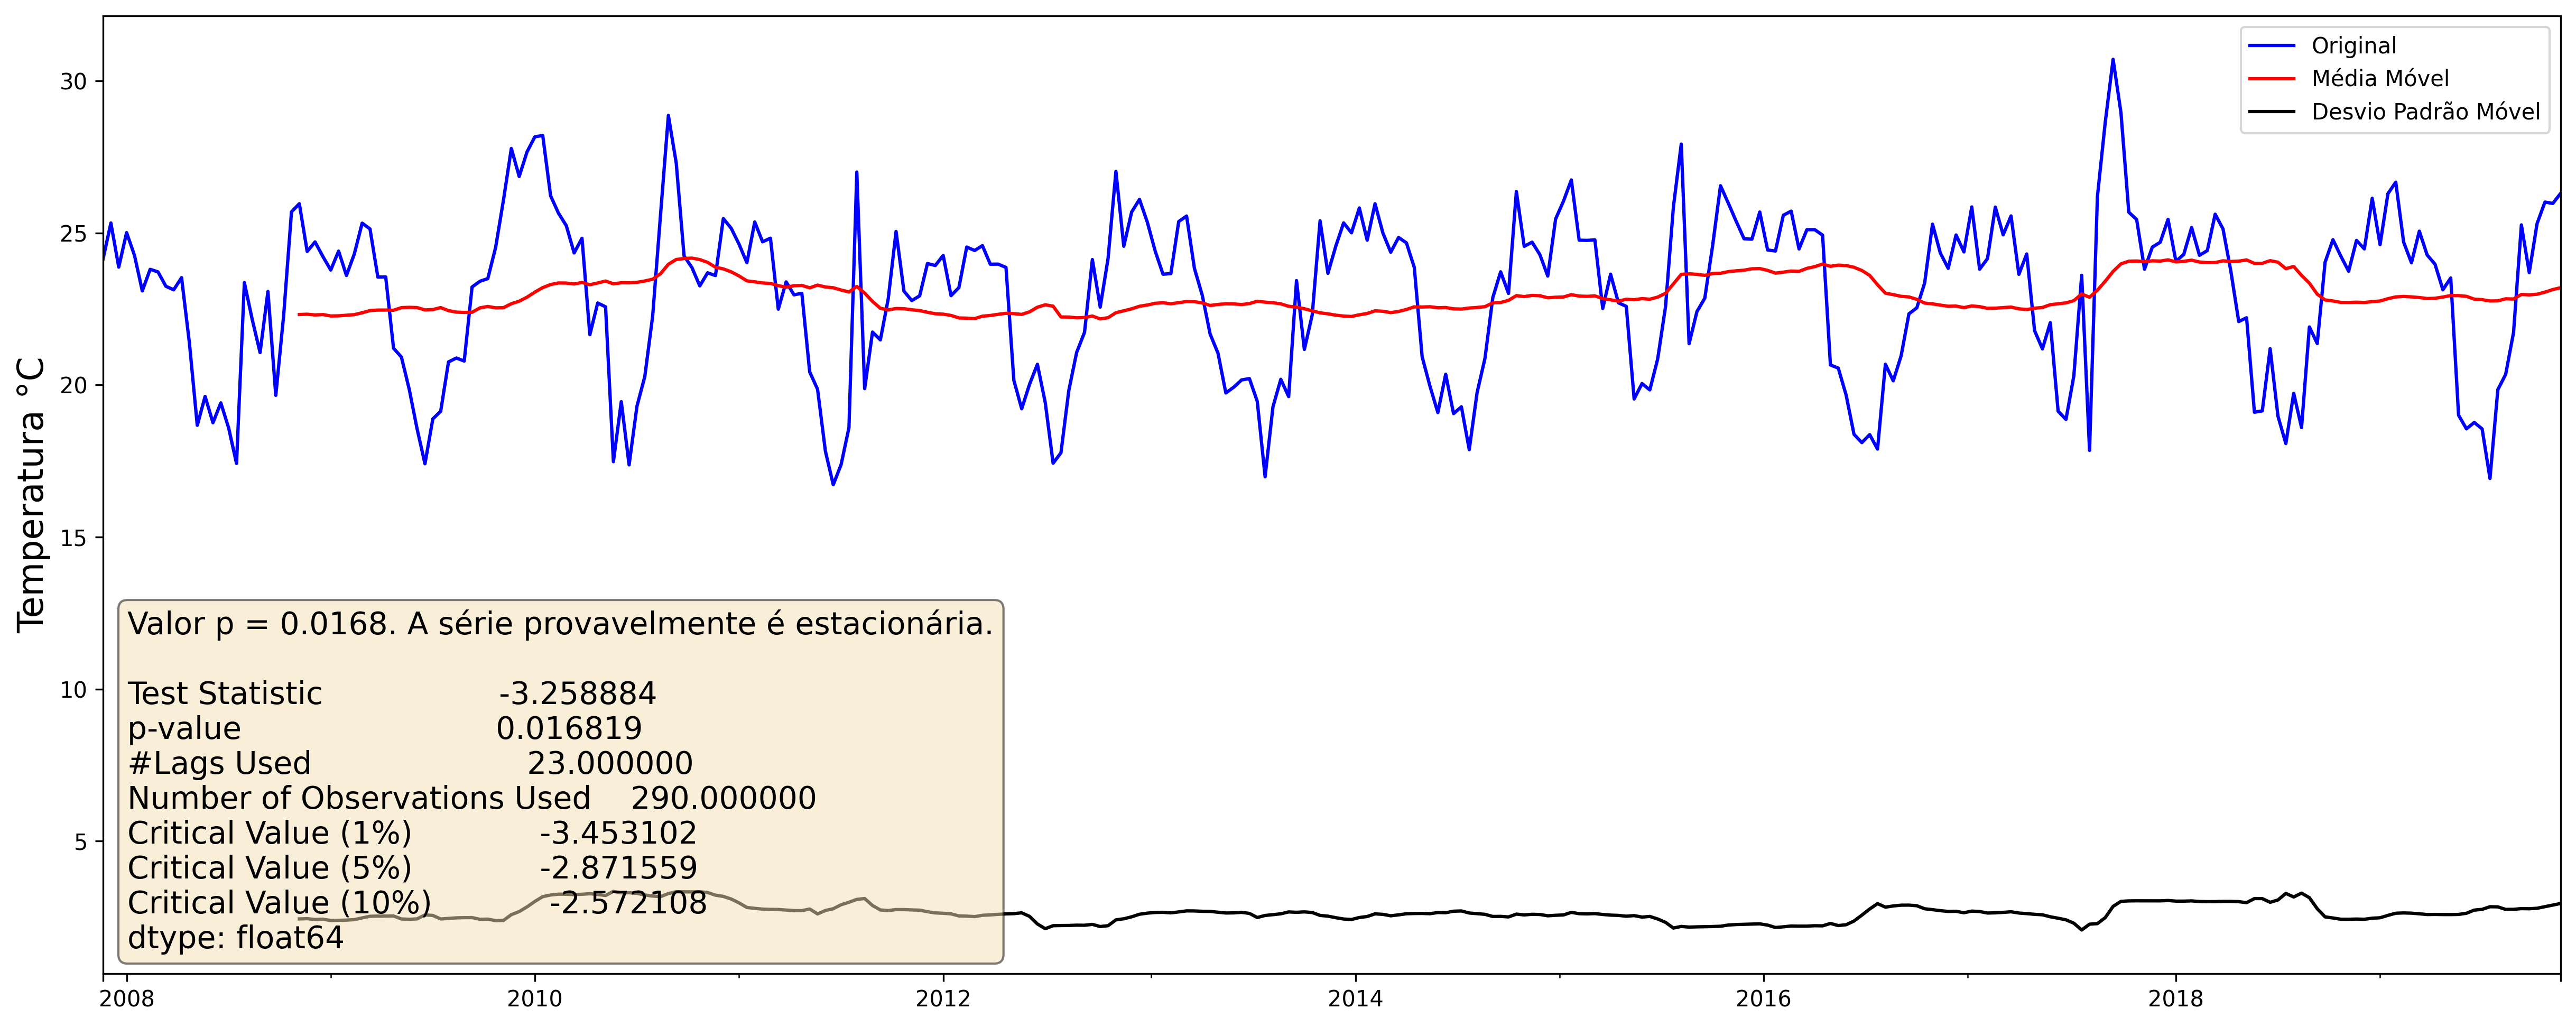
\includegraphics[width=0.9\textwidth]{figuras/dickey_fuller_raw_A736.png}
    \label{fig:estacionalidade_seria_original_2}
\end{figure}

\begin{figure}[H]
    \centering
    \caption{Teste de estacionalidade da série temporal da temperatura do ar para a estação automática localizada no município de Petrolina, no estado de Pernambuco.}
    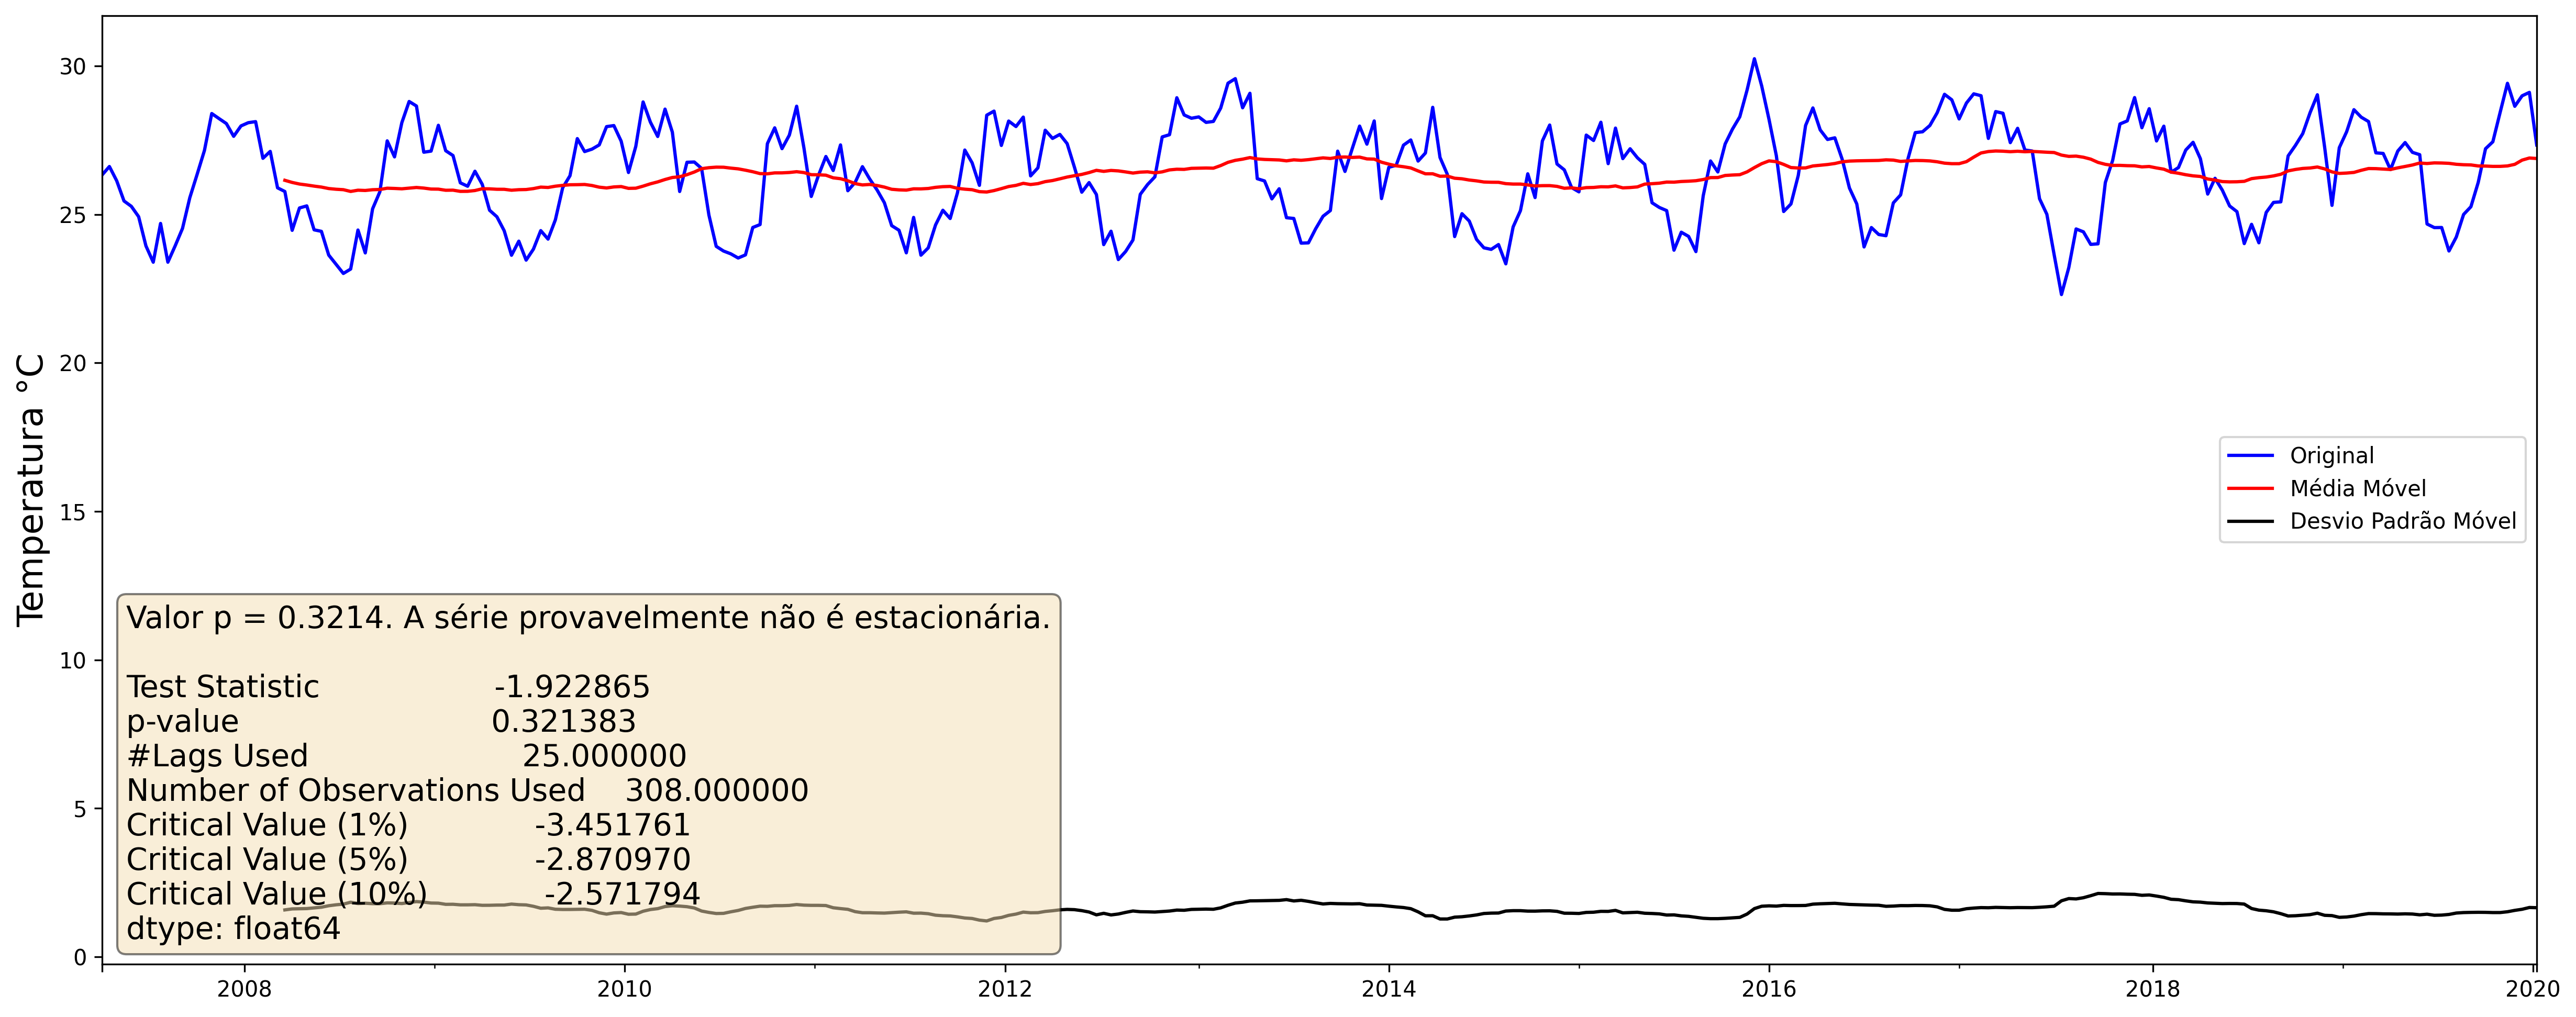
\includegraphics[width=0.9\textwidth]{figuras/dickey_fuller_raw_712f3e11658051636f09732a60fb3c1b.png}
    \label{fig:estacionalidade_seria_original_3}
\end{figure}

Pelo valor de p ser maior que 0,05, podemos afirmar que a primeira e a última série não são estacionarias, enquanto a segunda série, com o valor de p próximo de ~0,01, indica que a série é estacionária. Para garantirmos que todas as séries utilizadas por nosso modelo sejam estacionárias, aplicamos uma diferenciação de primeira ordem com o objetivo de trona-las todas séries estacionarias. 

Após o processo de diferenciação, realizamos novamente o teste de Dickey-Fuller aumentado e obtivemos os resultados apresentados das figuras \ref{fig:estacionalidade_seria_diferenciada_1}, \ref{fig:estacionalidade_seria_diferenciada_2} e \ref{fig:estacionalidade_seria_diferenciada_3}.  

\begin{figure}[H]
    \centering
    \caption{Teste de estacionalidade da série temporal diferenciada da temperatura do ar para a estação convencional localizada no município de Balsas, no estado do Maranhão.}
    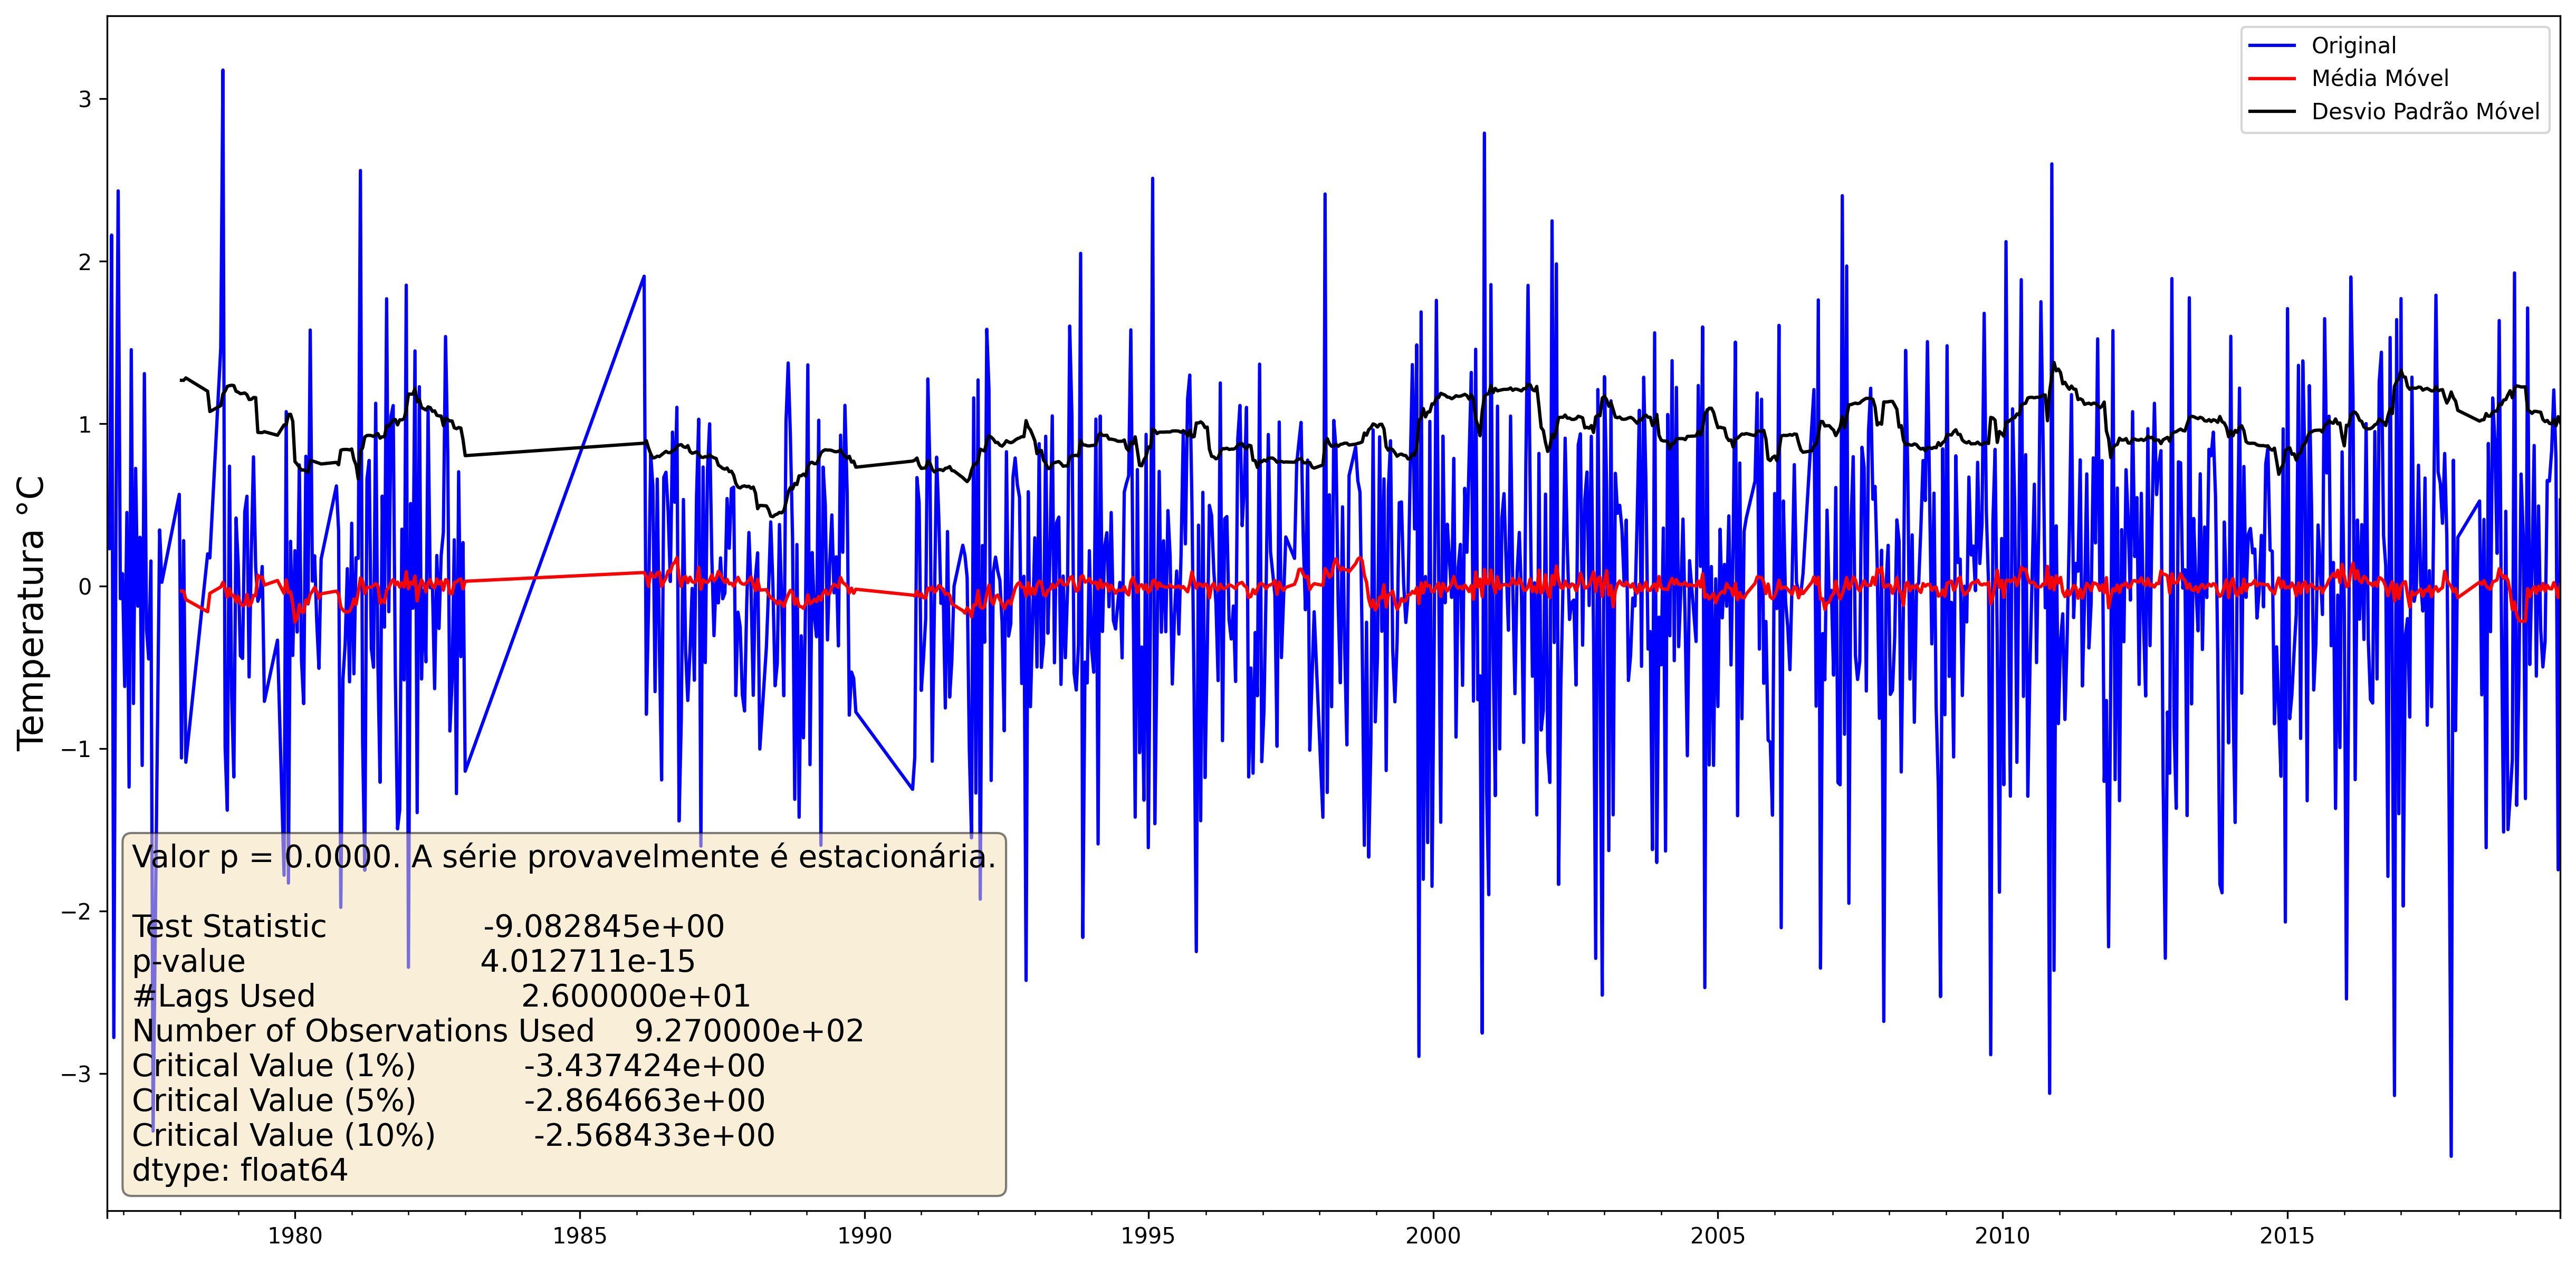
\includegraphics[width=0.9\textwidth]{figuras/dickey_fuller_diff_82768.png}
    \label{fig:estacionalidade_seria_diferenciada_1}
\end{figure}

\begin{figure}[H]
    \centering
    \caption{Teste de estacionalidade da série temporal diferenciada da temperatura do ar para a estação automática localizada no município de Ariranha, no estado de São Paulo.}
    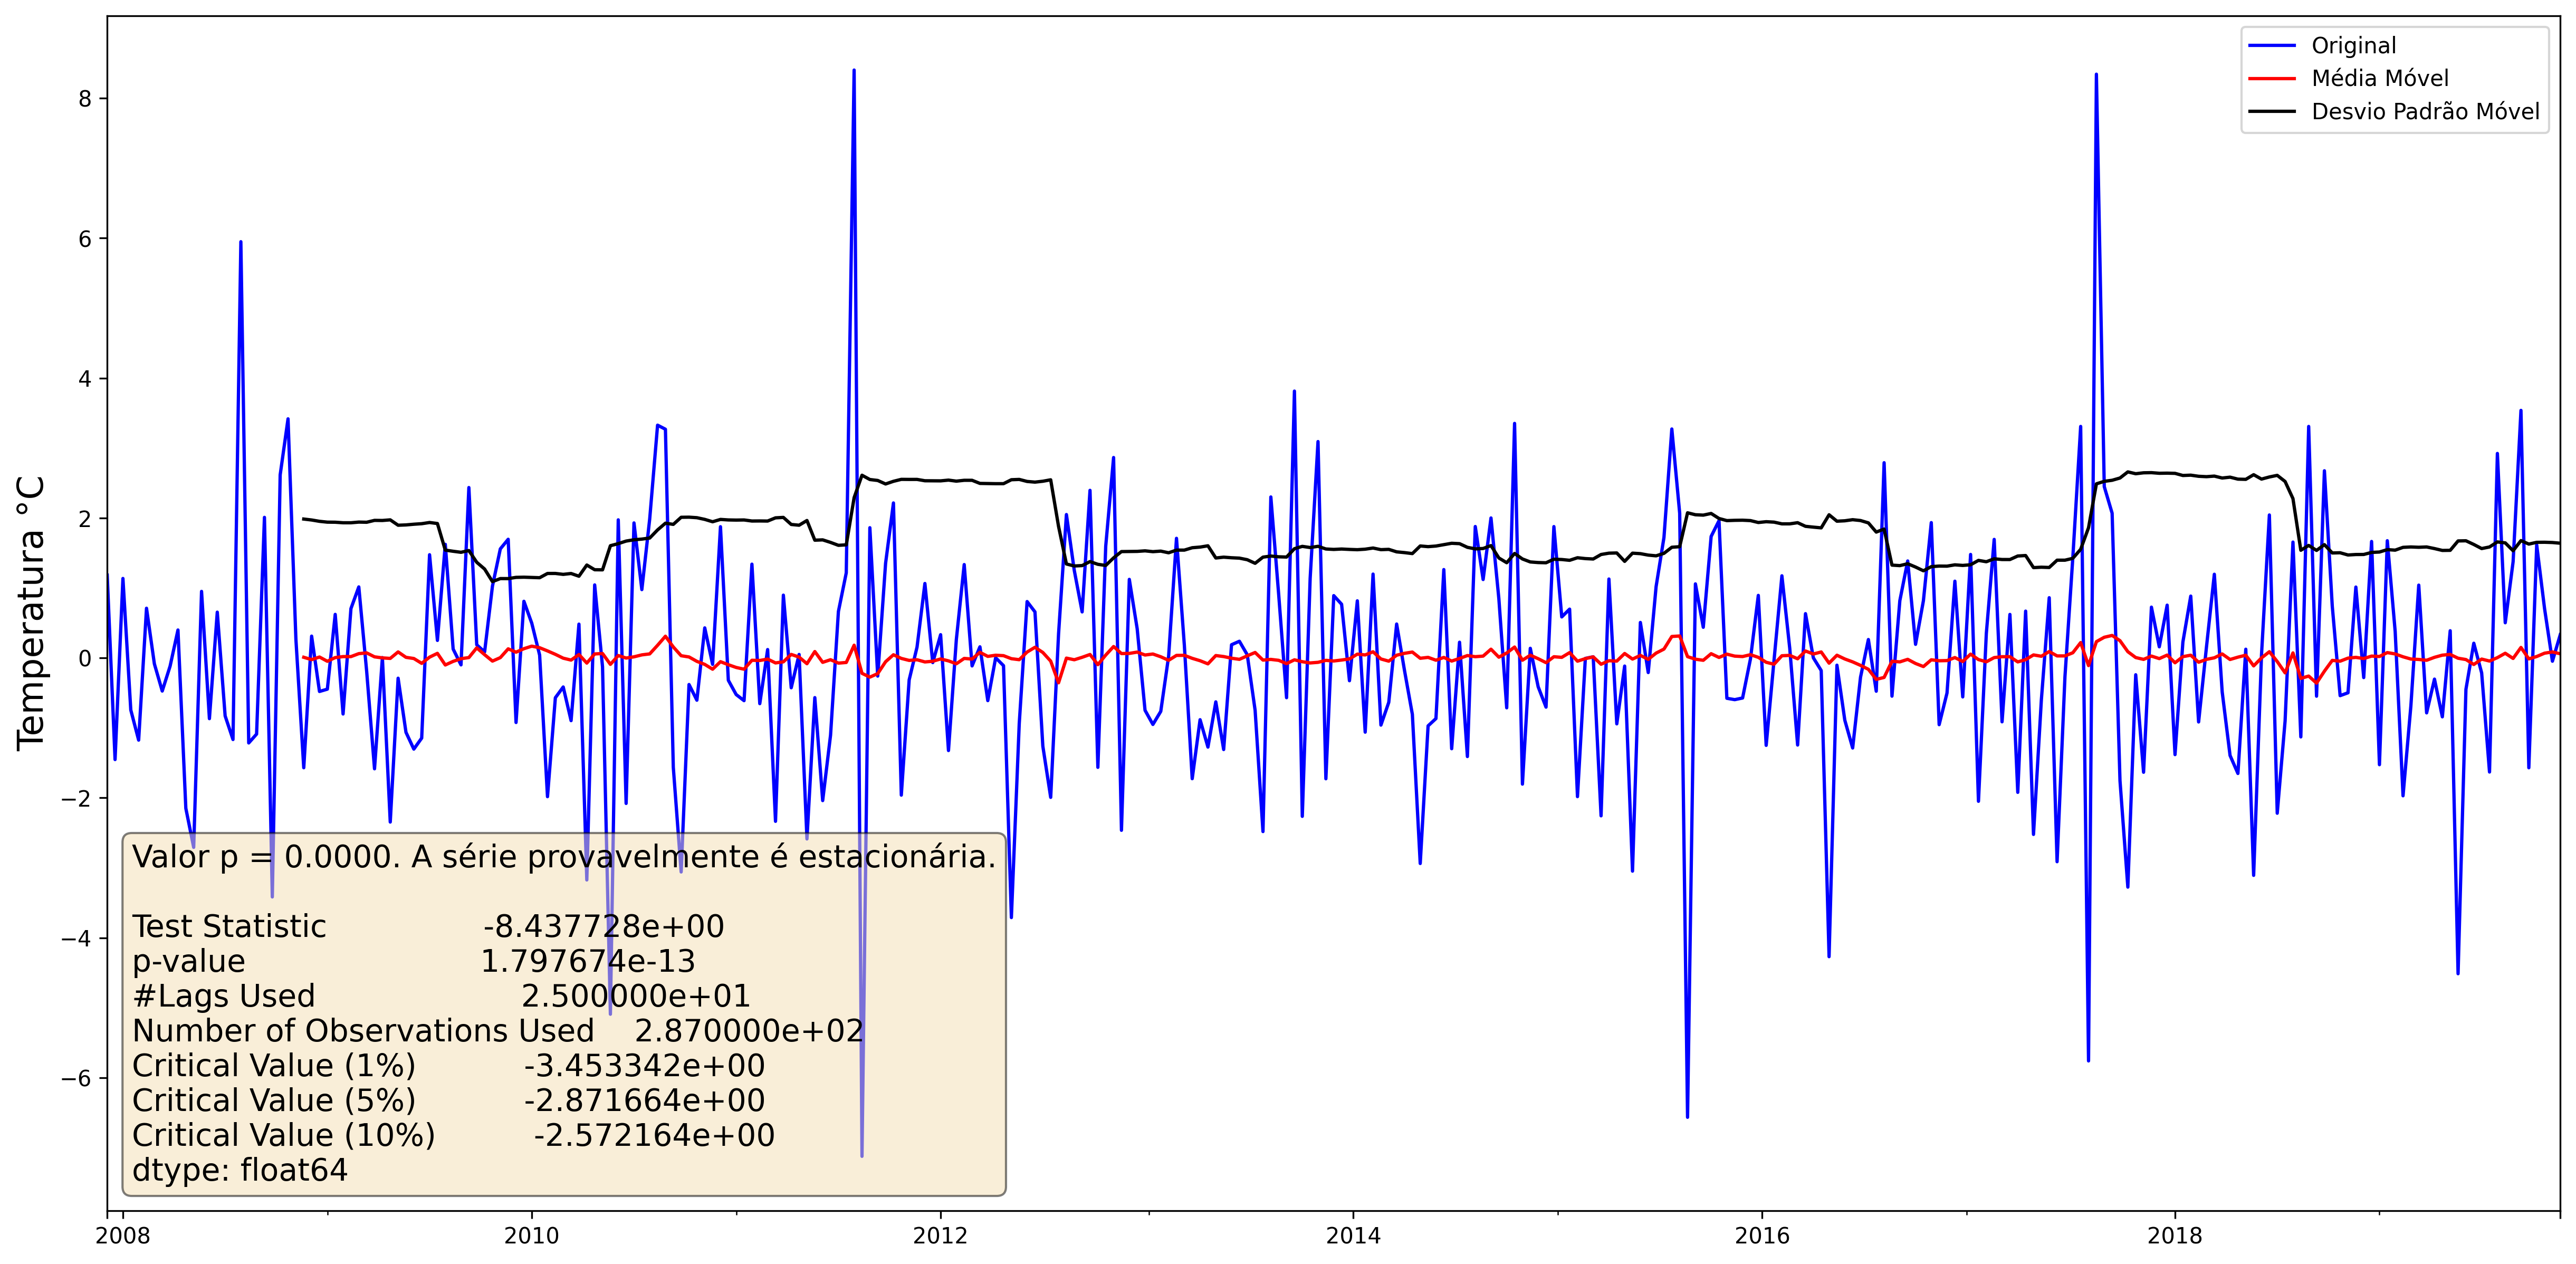
\includegraphics[width=0.9\textwidth]{figuras/dickey_fuller_diff_A736.png}
    \label{fig:estacionalidade_seria_diferenciada_2}
\end{figure}

\begin{figure}[H]
    \centering
    \caption{Teste de estacionalidade da série temporal diferenciada da temperatura do ar para a estação automática localizada no município de Petrolina, no estado de Pernambuco.}
    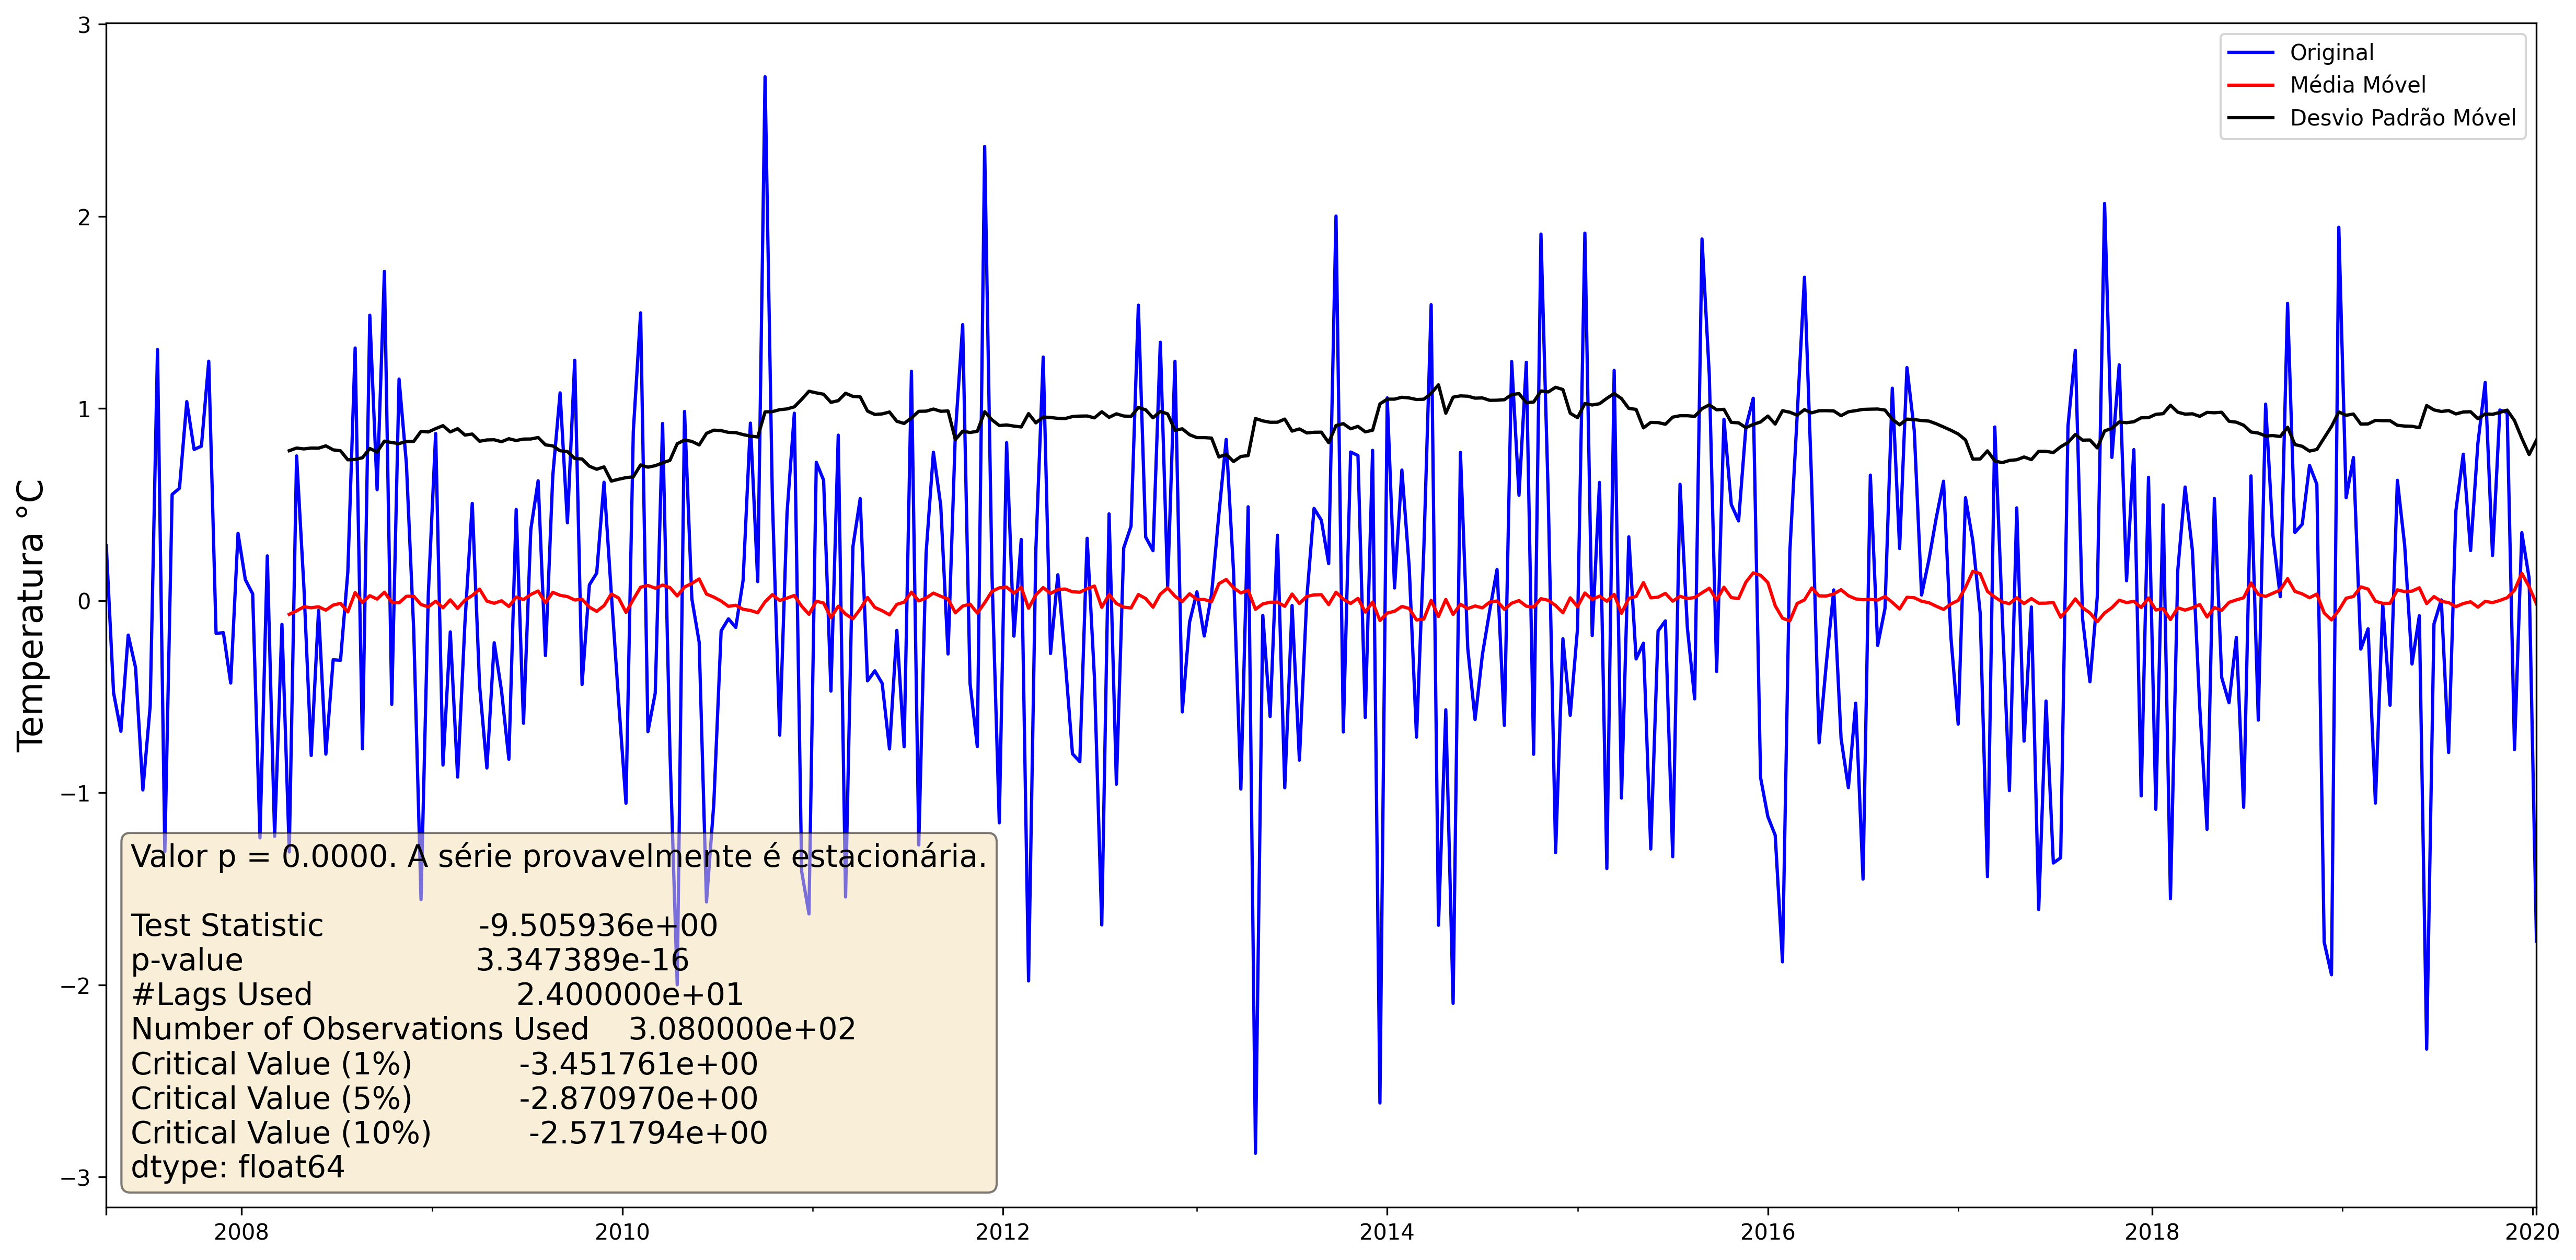
\includegraphics[width=0.9\textwidth]{figuras/dickey_fuller_diff_712f3e11658051636f09732a60fb3c1b.png}
    \label{fig:estacionalidade_seria_diferenciada_3}
\end{figure}

Após a diferenciação, todas as séries ficaram com o valor p abaixo de 0,05 e consequentemente passaram no teste da estacionalidade. Agora será possível parametrizarmos e treinarmos o modelo de previsão ARIMA. 

\subsection{Parametrizando o modelo ARIMA}

Para a parametrização do modelo, utilizamos a abordagem proposta por \cite{hyndman2007automatic}. Essa abordagem testa iterativamente um conjunto de parâmetros buscando encontrar a combinação que gera um modelo com o menor valor para a métrica Akaike information criterion (AIC) \cite{sakamoto1986akaike}, ou seja, ele buscar o melhor modelo ajustado sem ter que testar exaustivamente todas as combinações possíveis. Apesar dessa abordagem buscar o modelo com a melhor combinação de parâmetros, é necessário informar antecipadamente o intervalo de possíveis valores para os parâmetros que ele utilizará para testar os modelos. Apresentamos na Tabela \ref{tab:lista_parametros_arima} a lista dos principais parâmetros que serão ajustados.

\begin{table}[H]
\caption{Parâmetros do modelo que serão ajustados iterativamente.}
\label{tab:lista_parametros_arima}
\begin{adjustbox}{width=\textwidth}
\begin{tabular}{|l|l|}
\hline
\textbf{Nome do Parâmetro} & \textbf{Descrição}\\
\hline
p  & número de time lags do modelo auto-regressivo (AR) \\
\hline
q & ordem do modelo de média-móvel (MA) \\
\hline
d & grau de diferenciação \\
\hline
P & termo auto-regressivo para a parte sazonal \\
\hline
Q & termo da média-móvel para a parte sazonal \\
\hline
D & termo de diferenciação para a parte sazonal \\
\hline
\end{tabular}
\end{adjustbox}
\end{table}

Realizamos a busca pelo melhor modelo para cada uma das estações 88 estações selecionadas para análise. Para o processamento utilizamos a biblioteca escrita na linguagem Python pmdarima \cite{smith2017pmdarima}, versão 1.7.1. A Figura \ref{fig:parametros_auto_arima} apresenta todos parâmetros utilizados pela biblioteca pmdarima para buscar o melhor modelo para cada uma das estações avaliadas. 

\begin{figure}[H]
\centering
\caption{Parâmetros utilizados na função auto\_arima, da biblioteca pmdarima, para buscar o melhor modelo ajustado.}
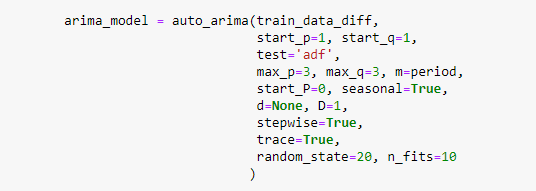
\includegraphics[width=0.9\textwidth]{figuras/parametros_autoarima.png}
\label{fig:parametros_auto_arima}
\end{figure}

\section{Criação do modelo LSTM}

As redes neurais recorrente do tipo Long Short-Term Memory (LSTM) tem a promessa de aprender longas sequências de observações, o que é desejável em nosso caso, já que possuímos algumas estações convencionais com observações que datam do ano 1961, ou seja, 58 anos de observações.  Mas para isso, elas exigem que sejam utilizados grandes conjuntos de dados de treinamento. Nesta seção,  apresentaremos a arquitetura desenvolvida e os passos executados para realizar as previsões utilizando este modelo. 

\subsection{Conjunto de dados de treinamento, validação e teste}

Para o treinamento e análise da acurácia do modelo, os dados foram separados em três conjuntos distintos, treinamento, validação e teste. Segundo \citeonline{hastie2009elements}, o conjunto de treinamento deve é usado para ajustar o modelo; o conjunto de validação deve usado para estimar o erro da predição do modelo e o conjunto de teste deve ser utilizado para avaliação o erro da generalização do modelo final escolhido. 

Para o conjunto de teste, assim como no modelo ARIMA, utilizamos as 88 estações que selecionamos na Figura \ref{tab:amostra_estacoes} como amostras para a avaliação dos modelos. O conjunto de treinamento e validação geramos a partir das estações restantes, ou seja, de todas as 878 estações, utilizamos mesma 88, que foram utilizadas no modelo ARIMA,  para a geração dos dados de teste e as 788 estações restantes utilizamos para o treinamento e validação do modelo LSTM.

O nosso modelo recebera como dado de entrada, chamaremos de X, uma série de observações de temperatura e retornará como previsão, chamaremos aqui de Y, os valores de temperatura média previstos para o próximo ano. Para criarmos um grande conjunto de dados de treinamento, ao invés de dividirmos uma série temporal em um único par (X, Y) utilizando Y como o último ano e X como os dados dos anos anteriores, vamos utilizar aqui deslocamentos de um ano na série para obtermos, de uma única série, múltiplos pares (X, Y). Na Tabela \ref{tab:dados_de_treinament_lstm} apresentamos todos os períodos utilizados para gerar os valores (X, Y) que foram utilizados para treinar o modelo LSTM. 

\begin{table}[H]
\centering
\caption{Quantidade de registros por conjunto de dados obtidos.}
\label{tab:dados_de_treinament_lstm}
\begin{adjustbox}{width=\textwidth}
\begin{tabular}{|l|l|}
\hline
\textbf{Período para obter o dado de entrada (X)} & \textbf{Período para obter a saída esperada (Y)}\\
\hline
todos os dados antes de 01/01/2019  & 01/01/2019 - 31/12/2019 \\
\hline
todos os dados antes de 01/01/2018  & 01/01/2018 - 31/12/2018 \\
\hline
todos os dados antes de 01/01/2017  & 01/01/2017 - 31/12/2017 \\
\hline
todos os dados antes de 01/01/2016  & 01/01/2016 - 31/12/2016 \\
\hline
todos os dados antes de 01/01/2015  & 01/01/2015 - 31/12/2015 \\
\hline
todos os dados antes de 01/01/2014  & 01/01/2014 - 31/12/2014 \\
\hline
todos os dados antes de 01/01/2013  & 01/01/2013 - 31/12/2013 \\
\hline
todos os dados antes de 01/01/2012  & 01/01/2012 - 31/12/2012 \\
\hline
todos os dados antes de 01/01/2011  & 01/01/2011 - 31/12/2011 \\
\hline
todos os dados antes de 01/01/2010  & 01/01/2010 - 31/12/2010 \\
\hline
\end{tabular}
\end{adjustbox}
\end{table}

Após processar todos os períodos, obtivemos 5.137 séries os os valores  entrada (X) e 5.137 séries com os valores esperados. Destas, 75\% dos pares(X, Y) foram alocados no conjunto de treinamento e 25\% foram alocados no conjunto de validação.  


\subsection{Normalização dos dados}

Para normalizar os dados de treinamento, utilizamos a função MinMaxScaler da biblioteca sklearn \cite{pedregosa2011scikit}, própria para aprendizado de máquina. Essa função tem como objetivo mapear os dados a serem normalizados no intervalo [0, 1]. Dessa forma, o maior valor que será normalizado receberá o valor de 1, e o menor, o valor de 0, os valores intermediários serão transformados em números dentro desse intervalo.

\subsection{Modelo LSTM desenvolvido}

Para a construção do modelo, utilizamos a biblioteca TensorFlow, versão 2.3.0. O modelo desenvolvido utiliza duas camadas LSTM, com 128 neurônios do tipo LSTM cada. Como camada de saída utilizamos uma camada densamente conectada com  ativação linear e 26 neurônios, cada neurônio será responsável por prevê um dos 26 períodos de duas semanas que compõe o ano que será previsto pelo modelo. Configuramos o modelo para utilizar o otimizador Adam com taxa de aprendizado de 0,001. Como função de perda utilizamos o Mean Squared Error (MSE) e como métrica de avaliação o Mean Absolute Error (MAE). A Figura \ref{fig:modelo_lstm} ilustra o modelo completo desenvolvido. 

\begin{figure}[H]
\centering
\caption{Arquitetura LSTM desenvolvida.}
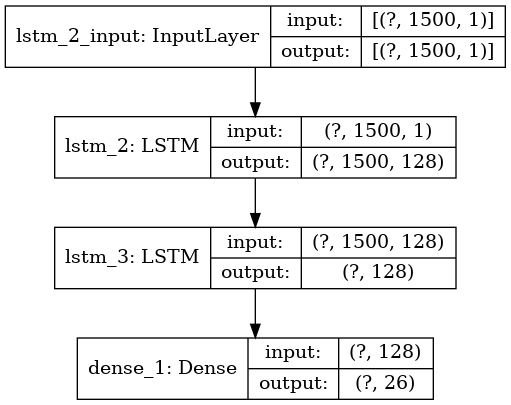
\includegraphics[width=0.7\textwidth]{figuras/lstm_model.png}
\label{fig:modelo_lstm}
\end{figure}

Para o treinamento do modelo, utilizamos lotes com 128 itens, treinando por 44 épocas. Utilizamos o \textit{callback} EarlyStopping do Keras para realizar uma parada precoce no treinamento com o objetivo de evitar ajustes excessivos no modelo. A Figura \ref{fig:perda_modelo} ilustra a perda do modelo ao longo do processo de treinamento. 

\begin{figure}[H]
\centering
\caption{Perda do modelo durante o processo de treinamento.}
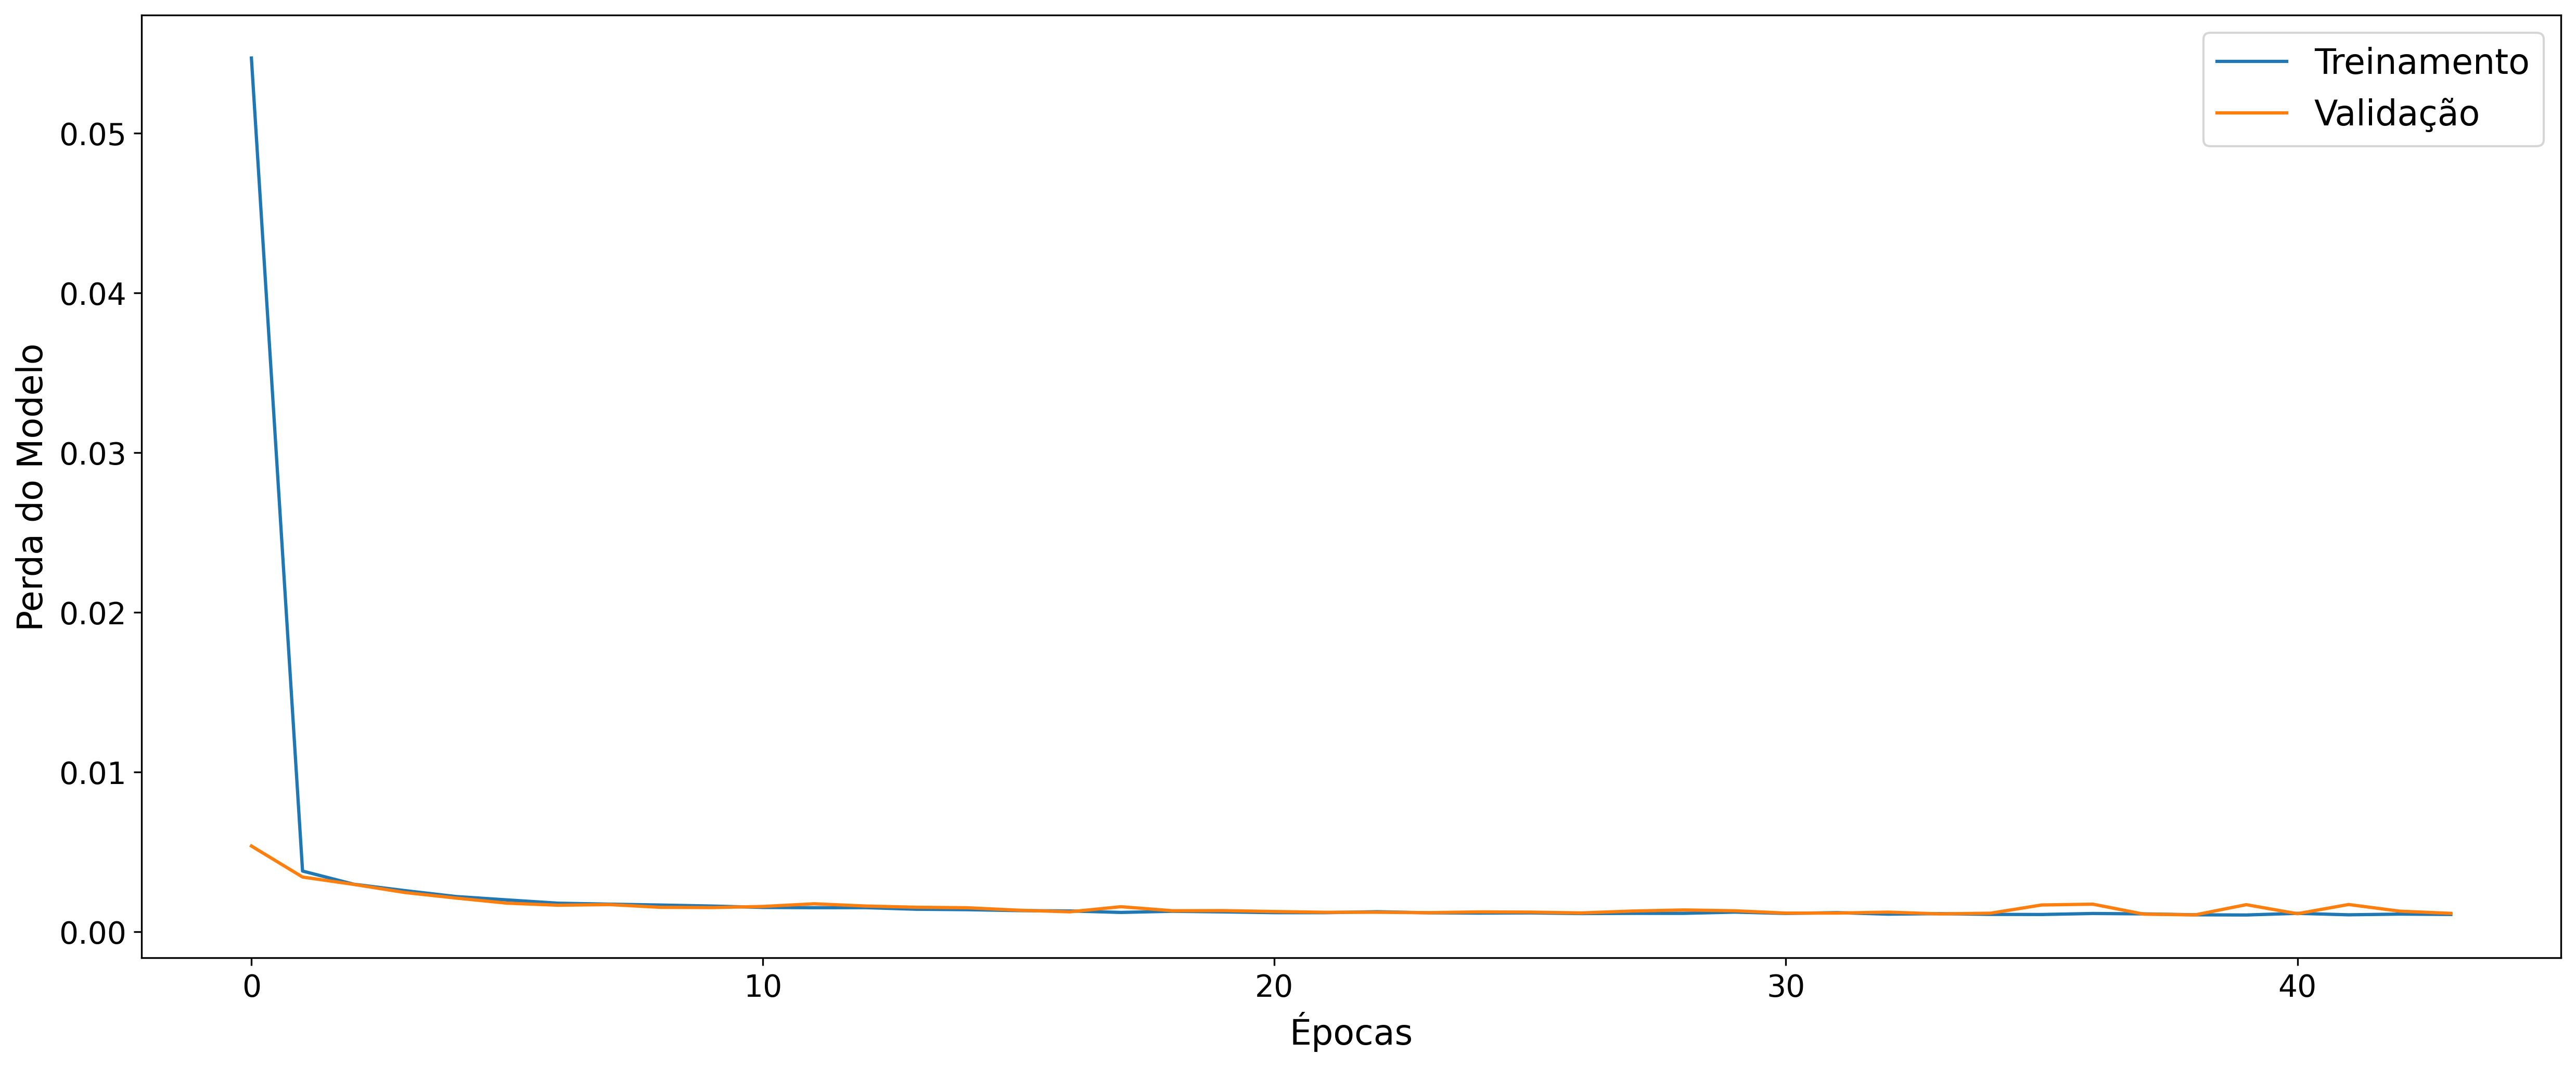
\includegraphics[width=\textwidth]{figuras/grafico_de_perda.png}
\label{fig:perda_modelo}
\end{figure}
\chapter{Apresentação dos Resultados}

Nessa seção, apresentaremos os resultados obtidos através dos modelos preditivos ARIMA e LSTM para a previsão da temperatura do ano de 2019. 

A Figura \ref{fig:results_histogram_arima_model_rmse} apresenta um histograma de comparação entre o erro médio quadrático (RMSE) obtido em cada um dos modelos, ARIMA e LSTM, para a previsão da temperatura do ano de 2019 nas 88 estações avaliadas. Analisando o gráfico podemos afirmar que o modelo LSTM obteve mais estações com os menores erros, abaixo de 1,5, enquanto que o modelo ARIMA apresentou mais estações com os maiores erros, acima de 2,0. Para todas as 88 estações avaliadas, o RMSE  Global, ou seja, a média de todos os erros, foi 2,67 para o modelo ARIMA e 1,38 para o modelo LSTM, indicando que o modelo LSTM obteve um desempenho, na previsão, melhor que o modelo ARIMA. 
 
 \begin{figure}[H]
    \centering
    \caption{Comparação entre os valores obtidos de RMSE para as 88 estações avaliadas.}
    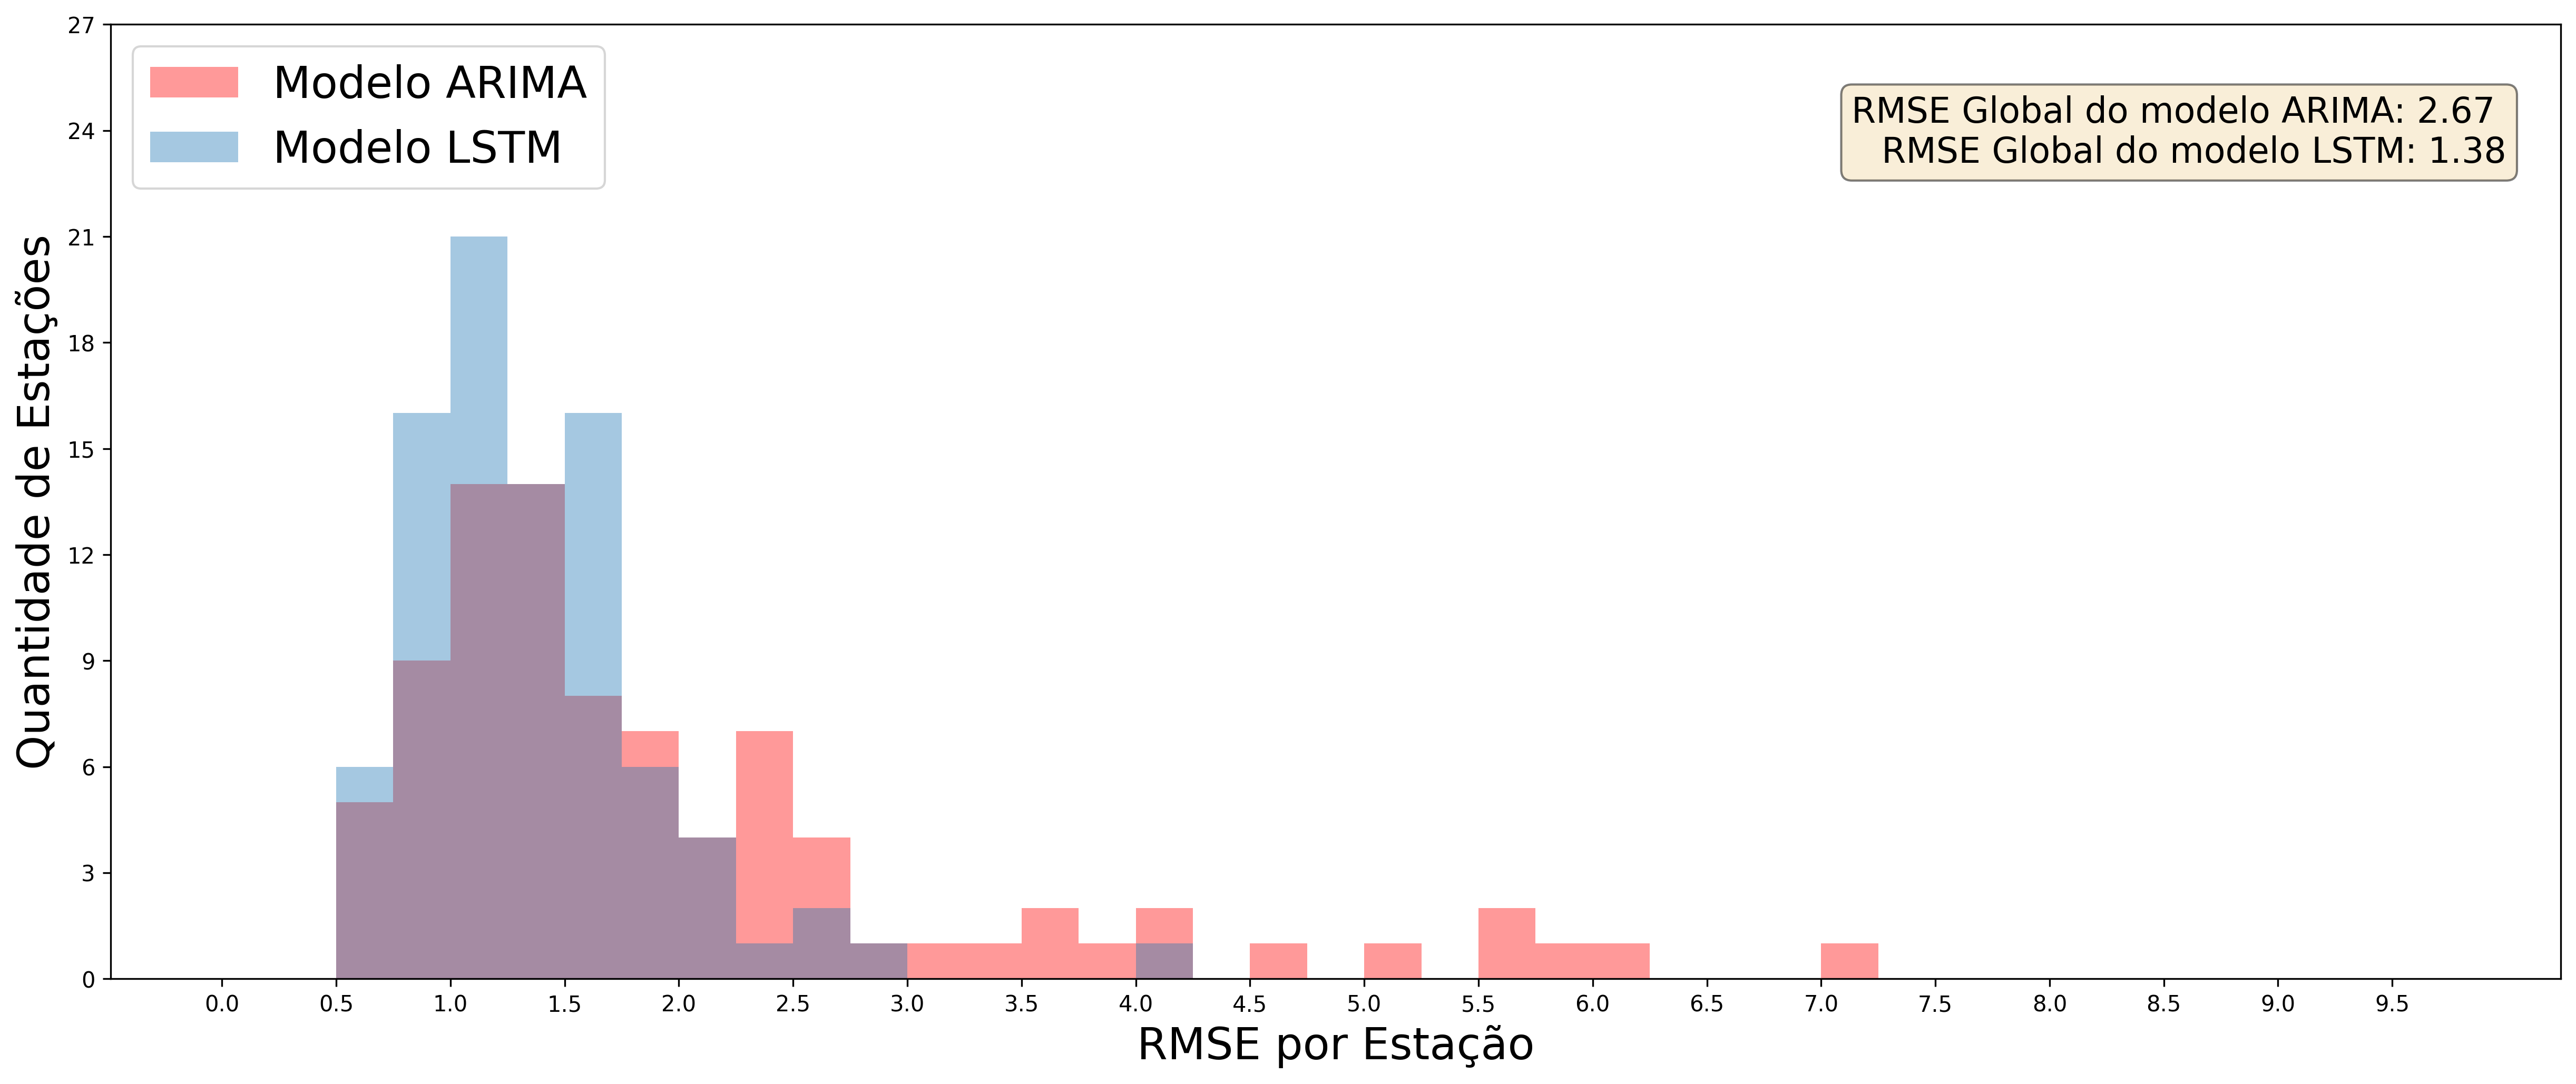
\includegraphics[width=\textwidth]{figuras/results/comparacao_rmse_arima_lstm_histograma.png}
    \label{fig:results_histogram_arima_model_rmse}
\end{figure}

Analisando as previsões individuais, ilustramos na Figura \ref{fig:results_arima_A826} o resultado da previsão para uma estação localizada no município de Alegrete, no estado do Rio Grande do Sul. 
Para esta estação em que o modelo ARIMA apresentou um maior erro, acima de 5, o modelo LSTM conseguiu uma boa performance alcançando um erro um pouco acima de 1,8. Esse comportamento se refletiu em diversas outras estações em que o modelo ARIMA obteve um resultado pior em relação ao seu próprio RMSE Global.  

\begin{figure}[H]%
\caption{Resultado da previsão da temperatura do ar para o ano de 2019 na estação meteorológica localizada no município de Alegrete, no estado do Rio Grande do Sul.}
\centering
\subfloat{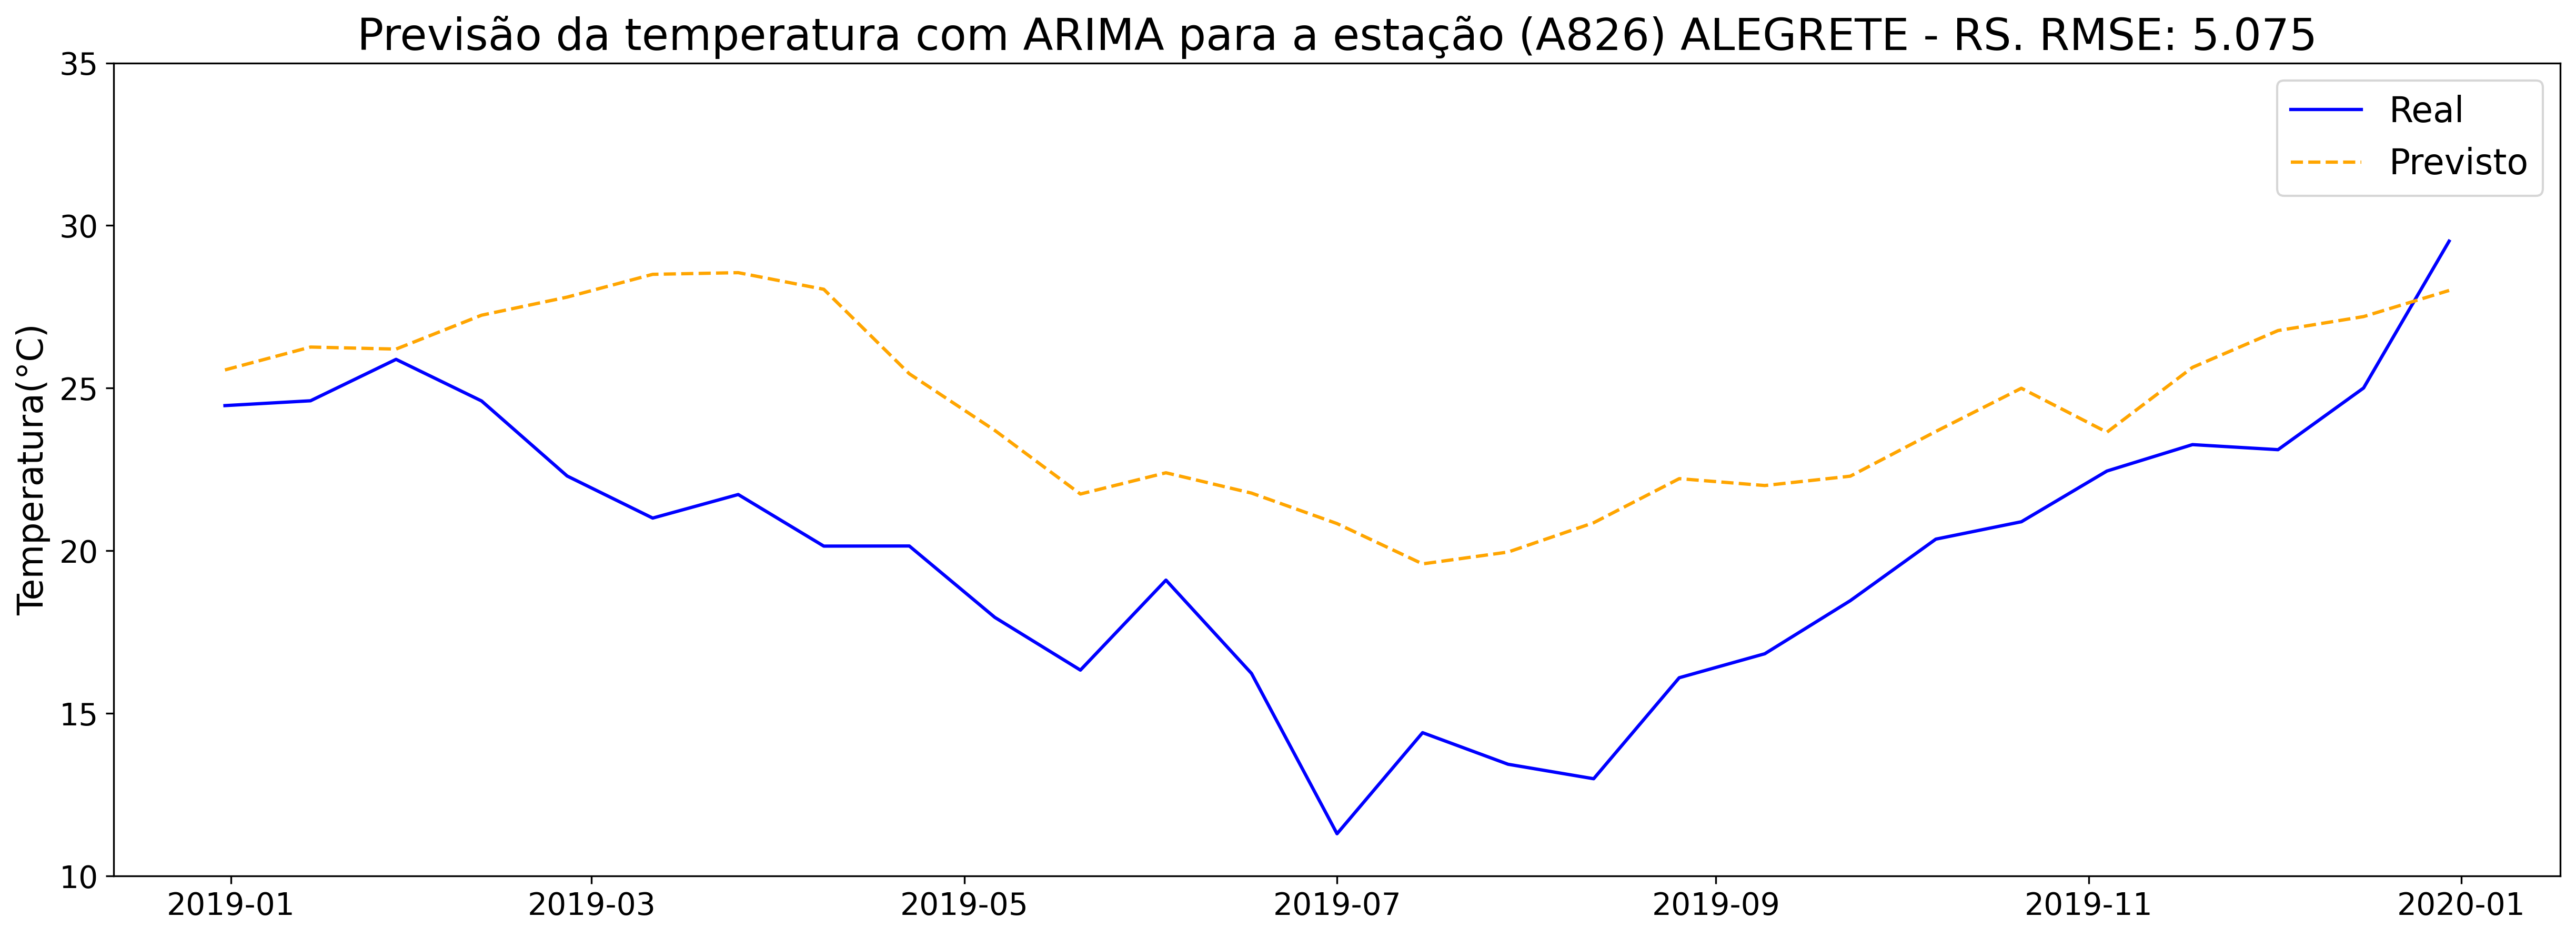
\includegraphics[scale=.30]{figuras/results/results_arima_A826.png}}
\qquad
\subfloat{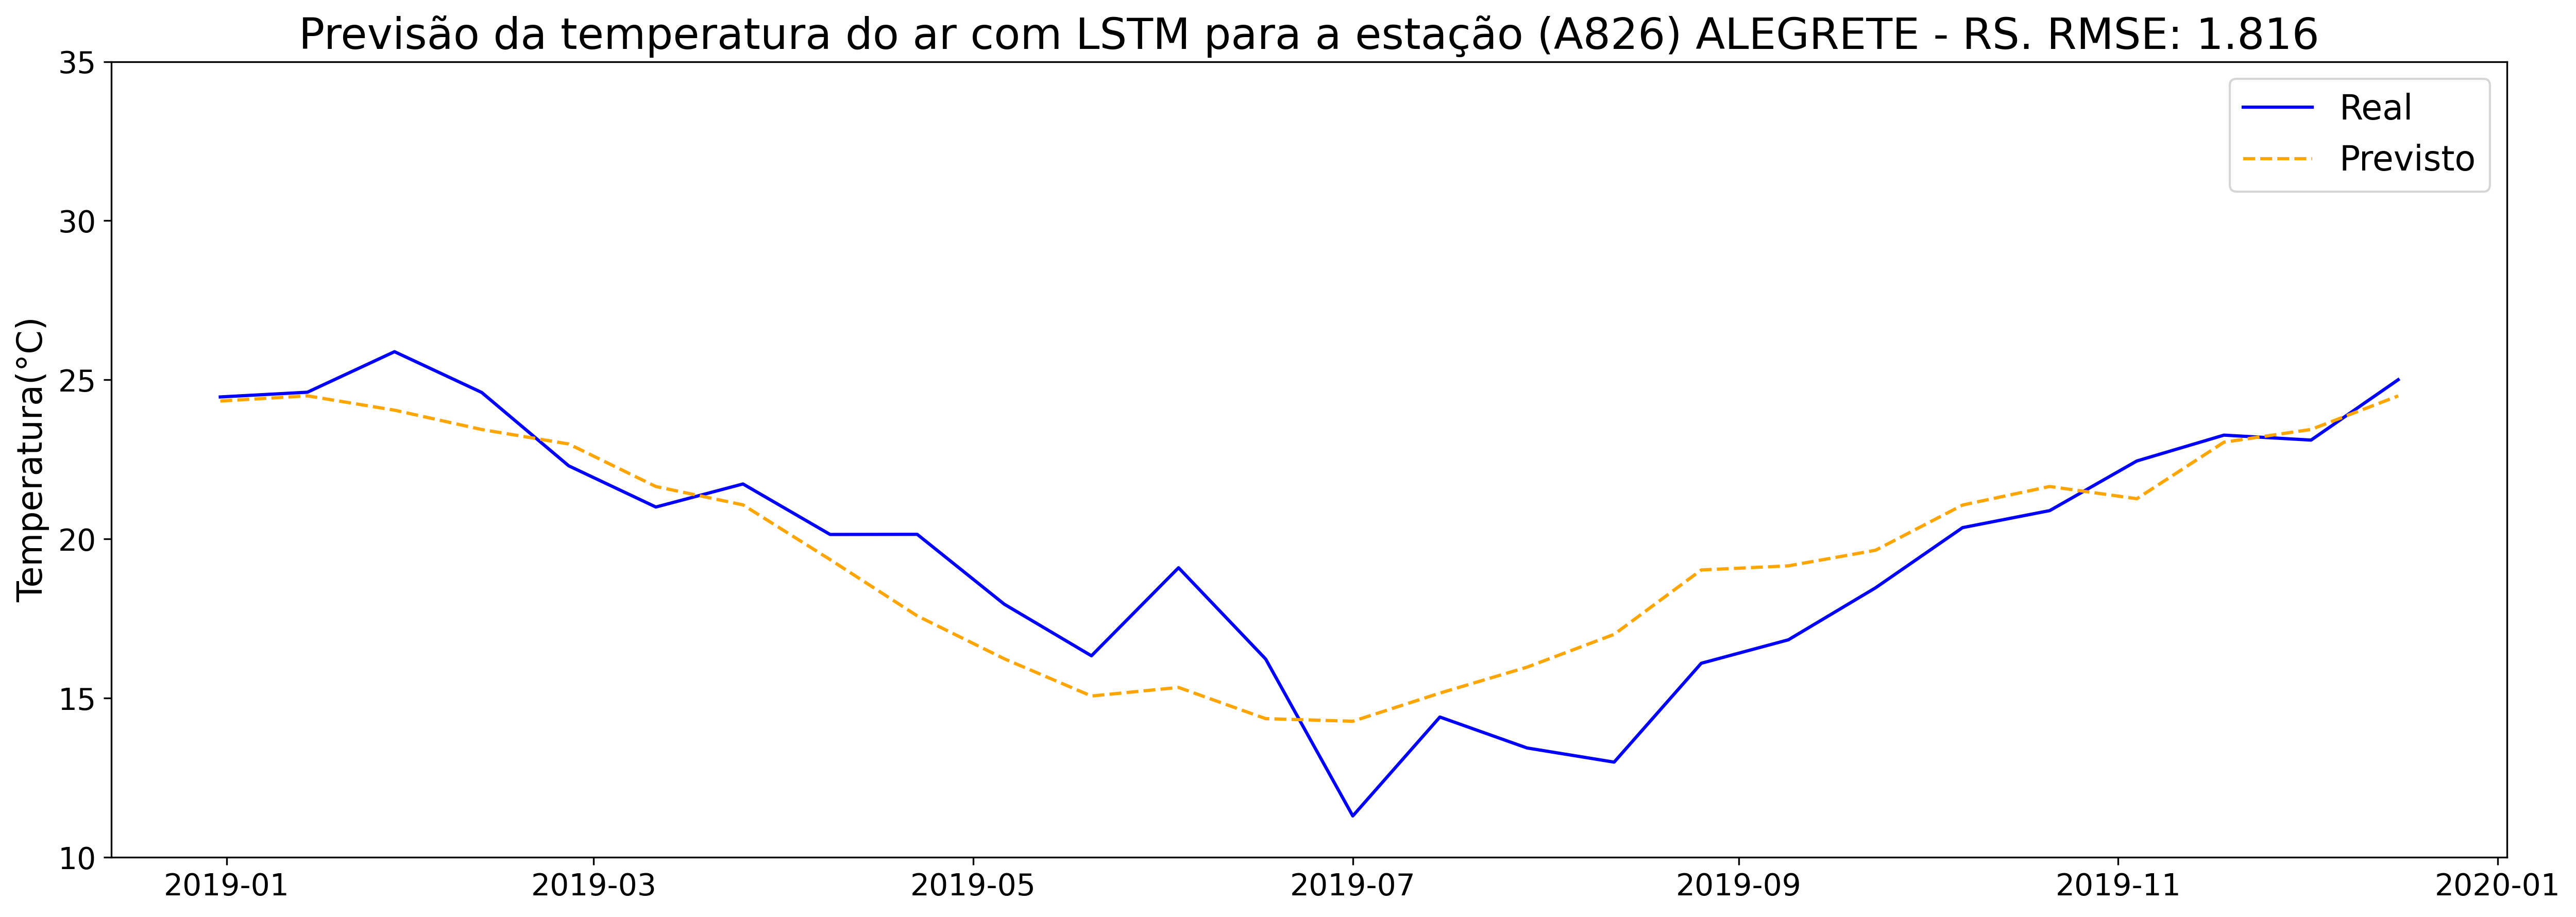
\includegraphics[scale=.30]{figuras/results/results_lstm_A826.png}}
\label{fig:results_arima_A826}%
\end{figure}

Avaliando as estações em que o modelo LSTM obteve um desempenho pior do que seu seu próprio RMSE Global, identificamos que, nessas estações, o modelo ARIMA não obteve grande vantagem, nas raras vezes em que foi melhor, em relação ao modelo LSTM. Na Figura \ref{fig:results_arima_A720} adicionamos um exemplo do resultado da previsão para uma estação em que o modelo LSTM não conseguiu bons resultados. Nas figuras \ref{fig:results_lstm_83464} e \ref{fig:results_lstm_83361} também apresentamos o resultados da previsão para outras estações. 

\begin{figure}[H]%
\caption{Resultado da previsão da temperatura do ar para o ano de 2019 na estação meteorológica localizada no município de Coxim, no estado do Mato Grosso do Sul.}
\centering
\subfloat{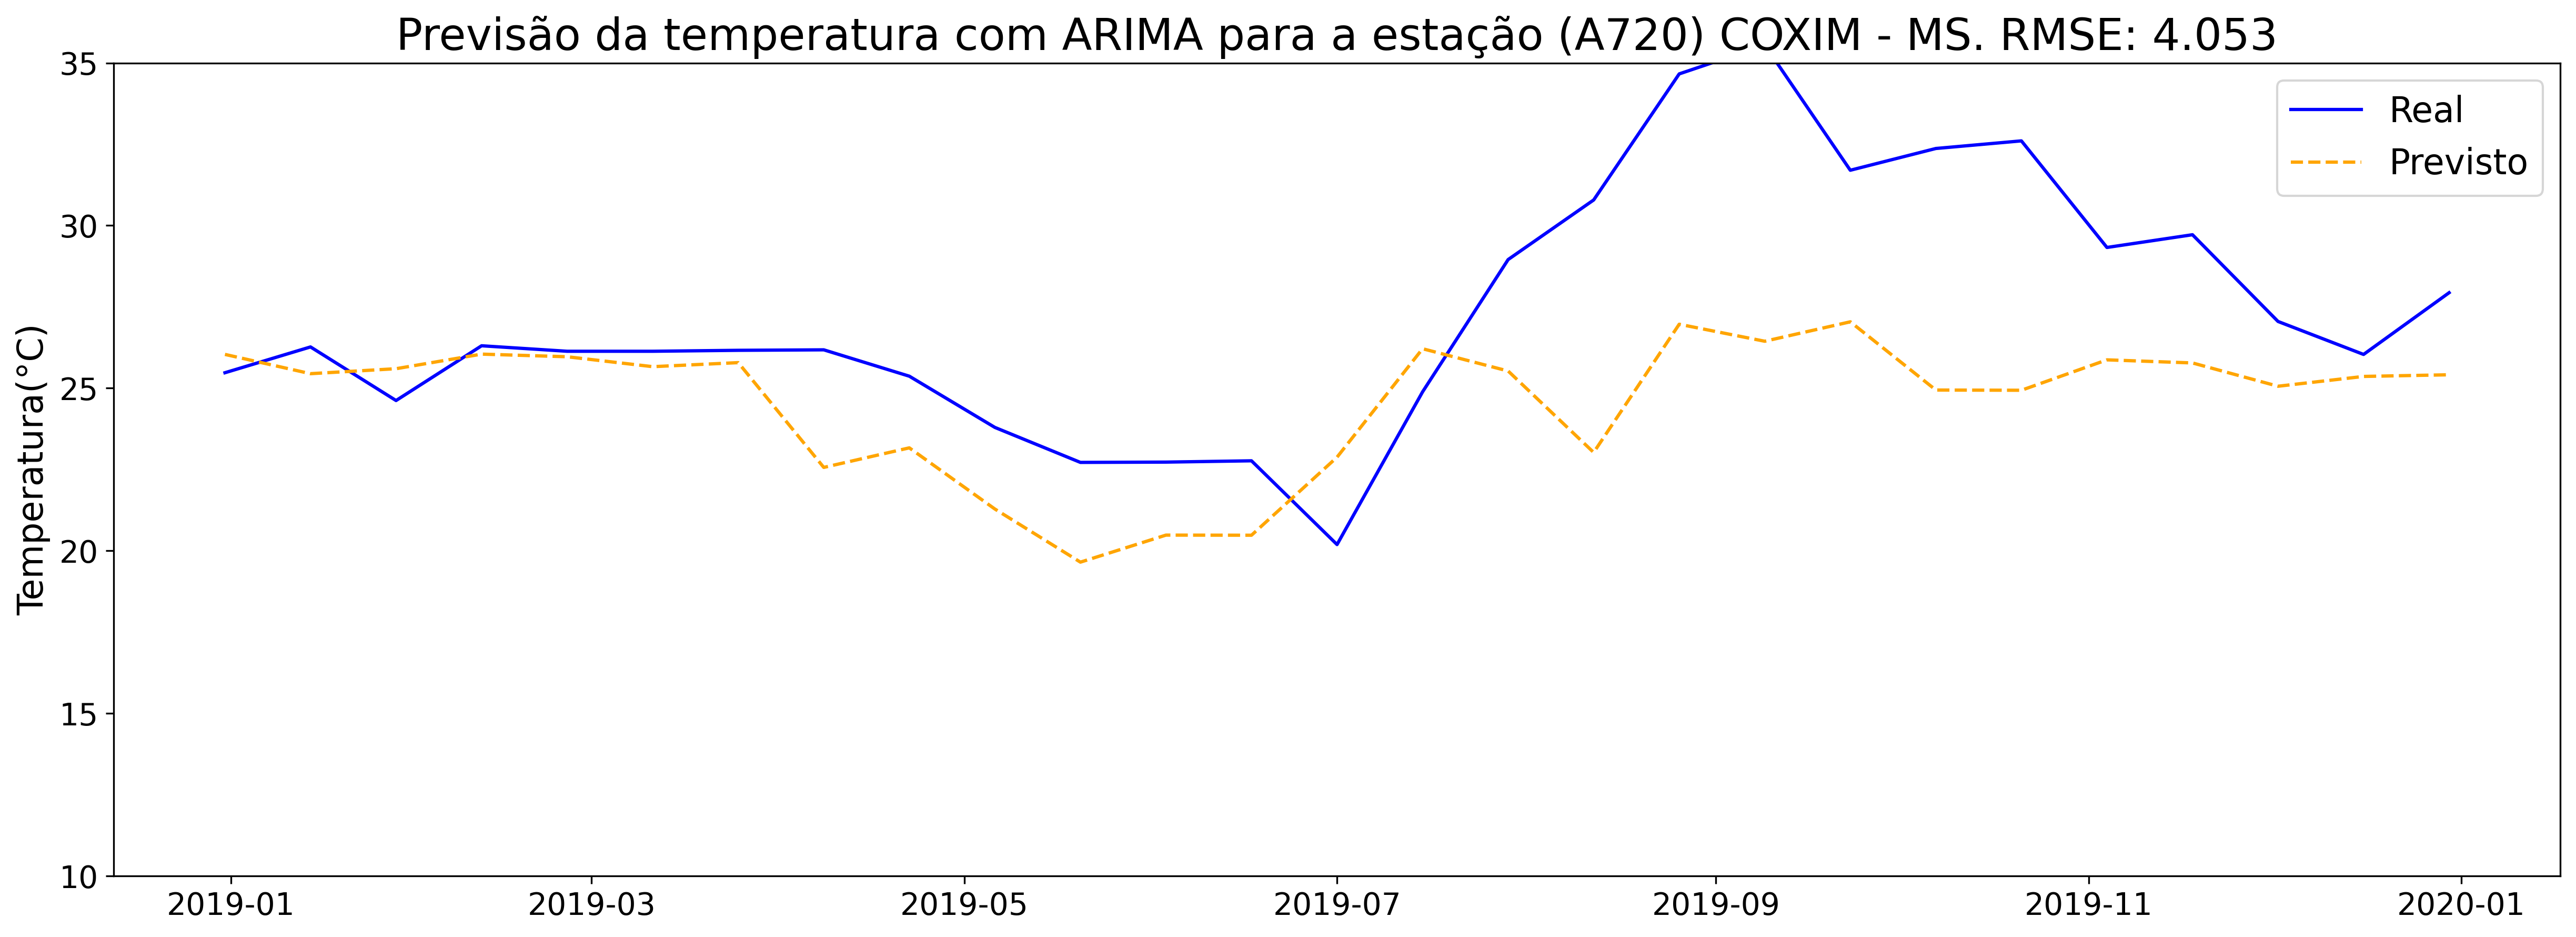
\includegraphics[scale=.30]{figuras/results/results_arima_A720.png}}
\qquad
\subfloat{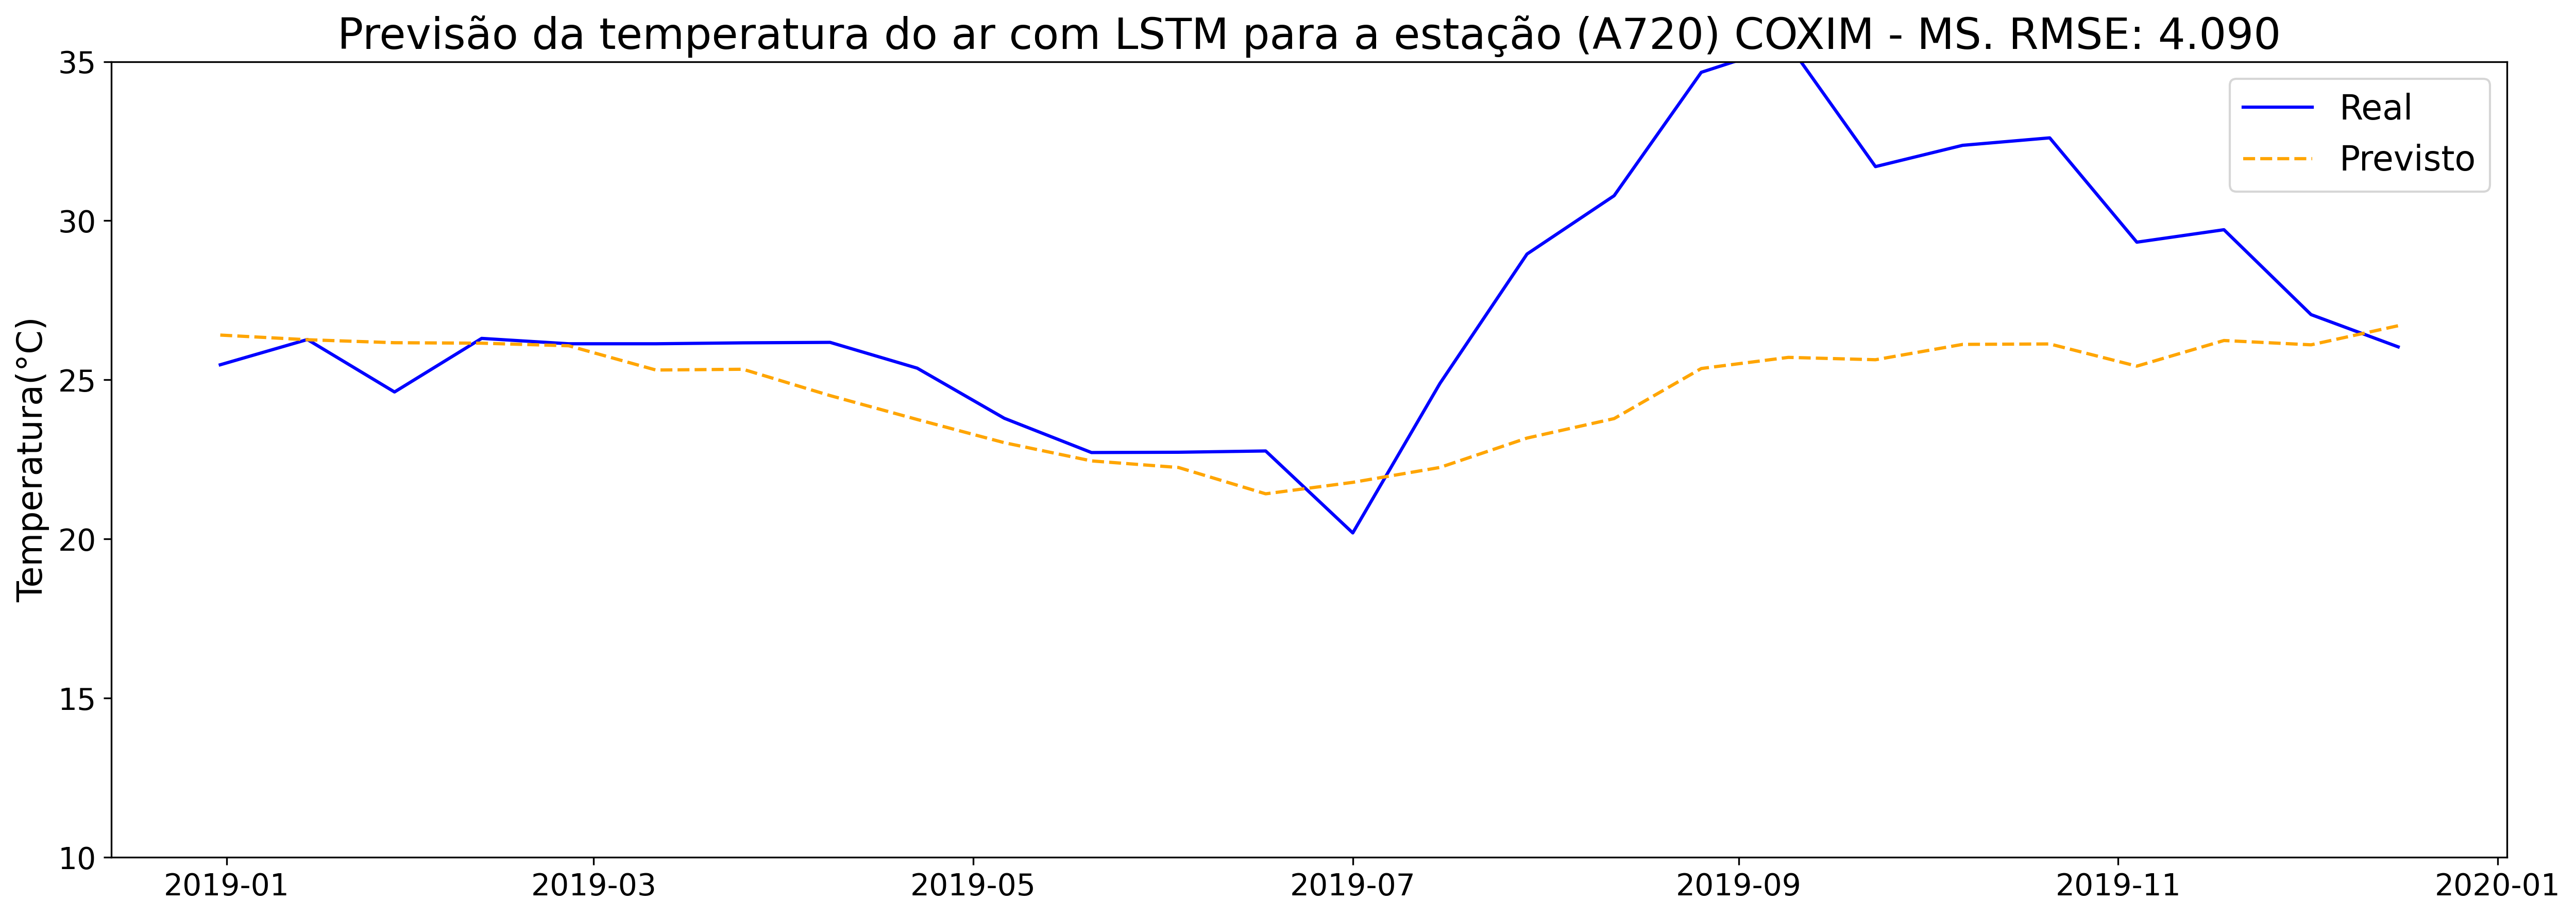
\includegraphics[scale=.30]{figuras/results/results_lstm_A720.png}}
\label{fig:results_arima_A720}%
\end{figure}

\begin{figure}[H]%
\caption{Resultado da previsão da temperatura do ar para o ano de 2019 na estação meteorológica localizada no município de Jataí, no estado de Goiás.}
\centering
\subfloat{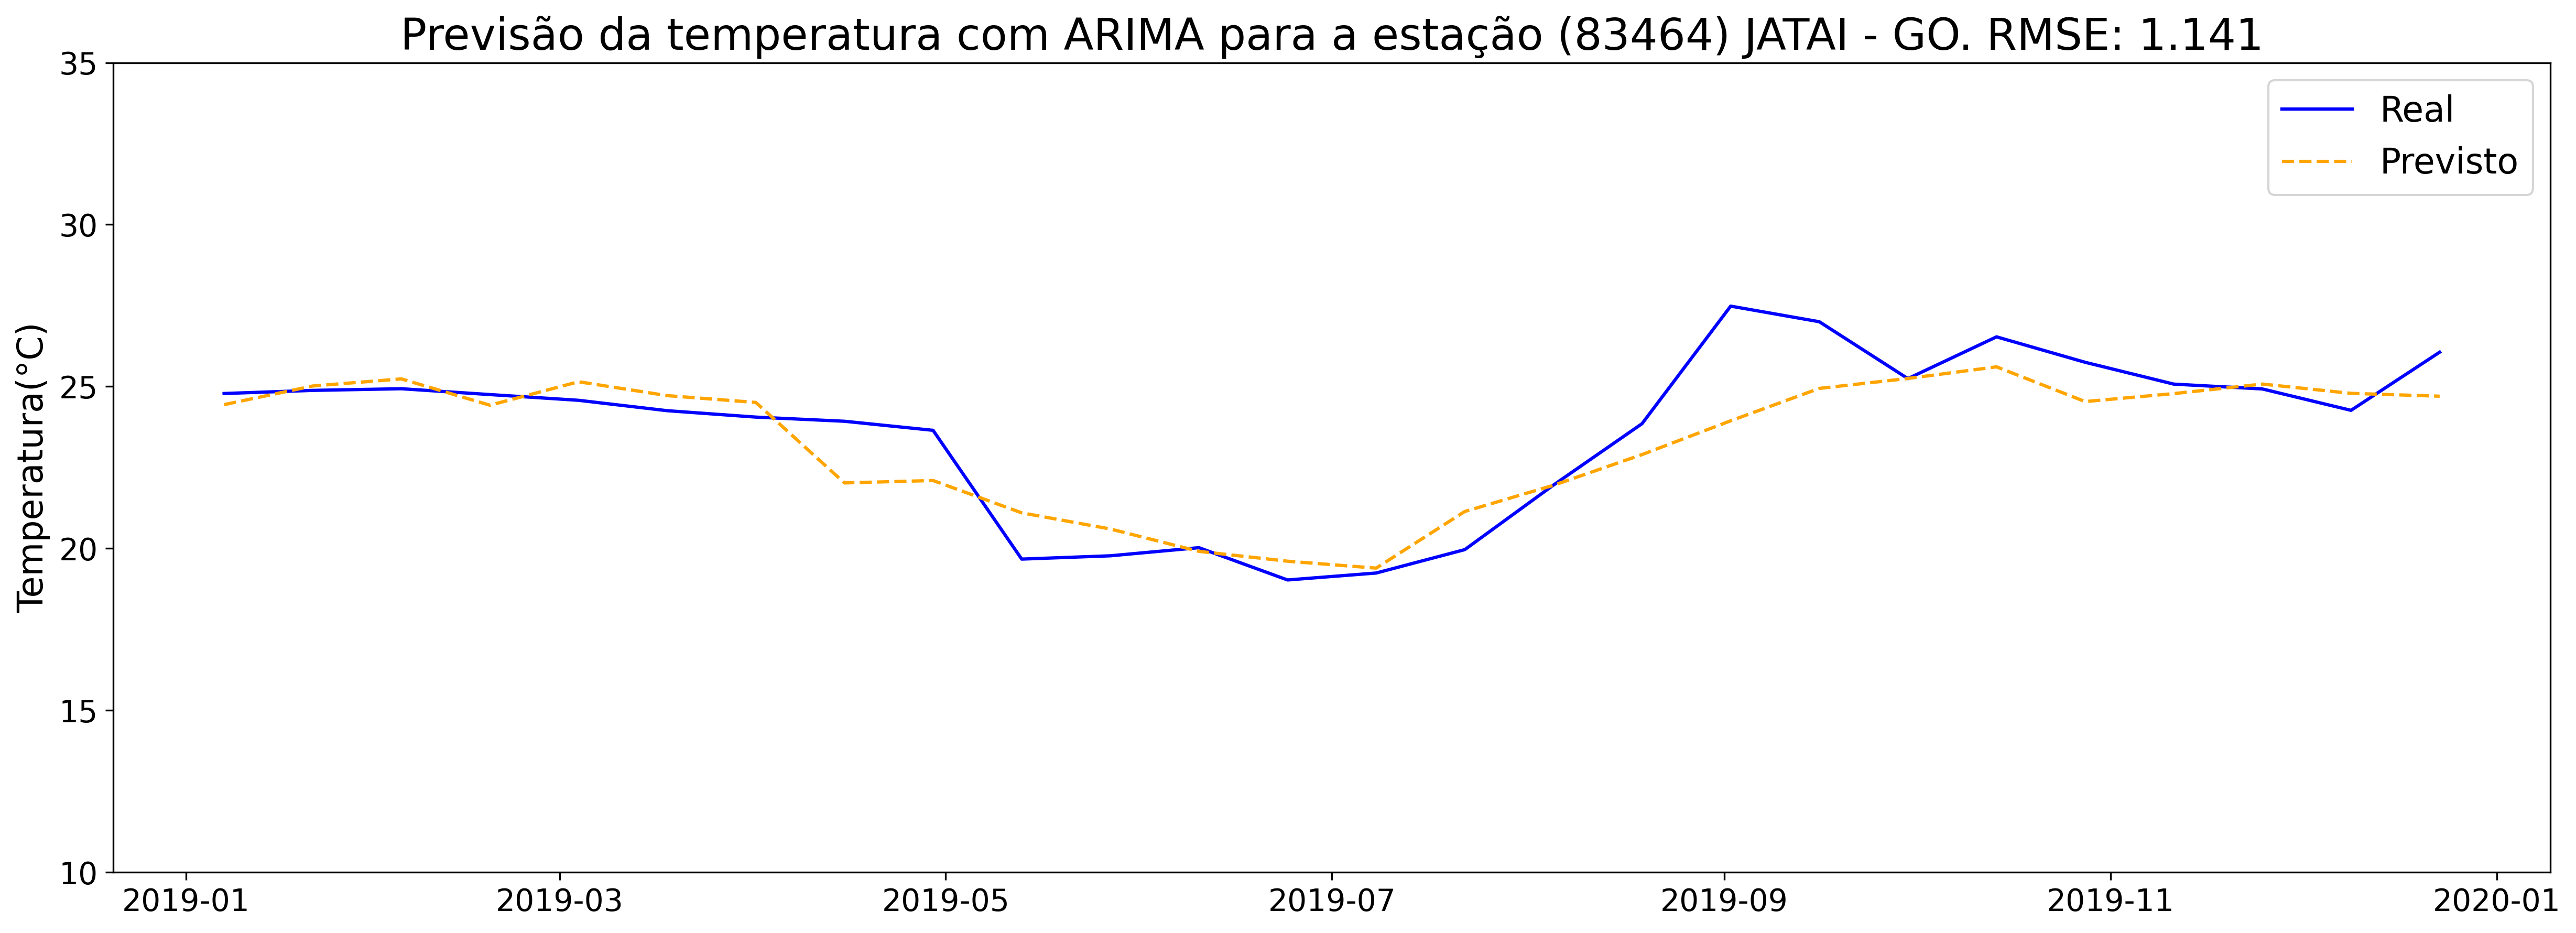
\includegraphics[scale=.30]{figuras/results/results_arima_83464.png}}
\qquad
\subfloat{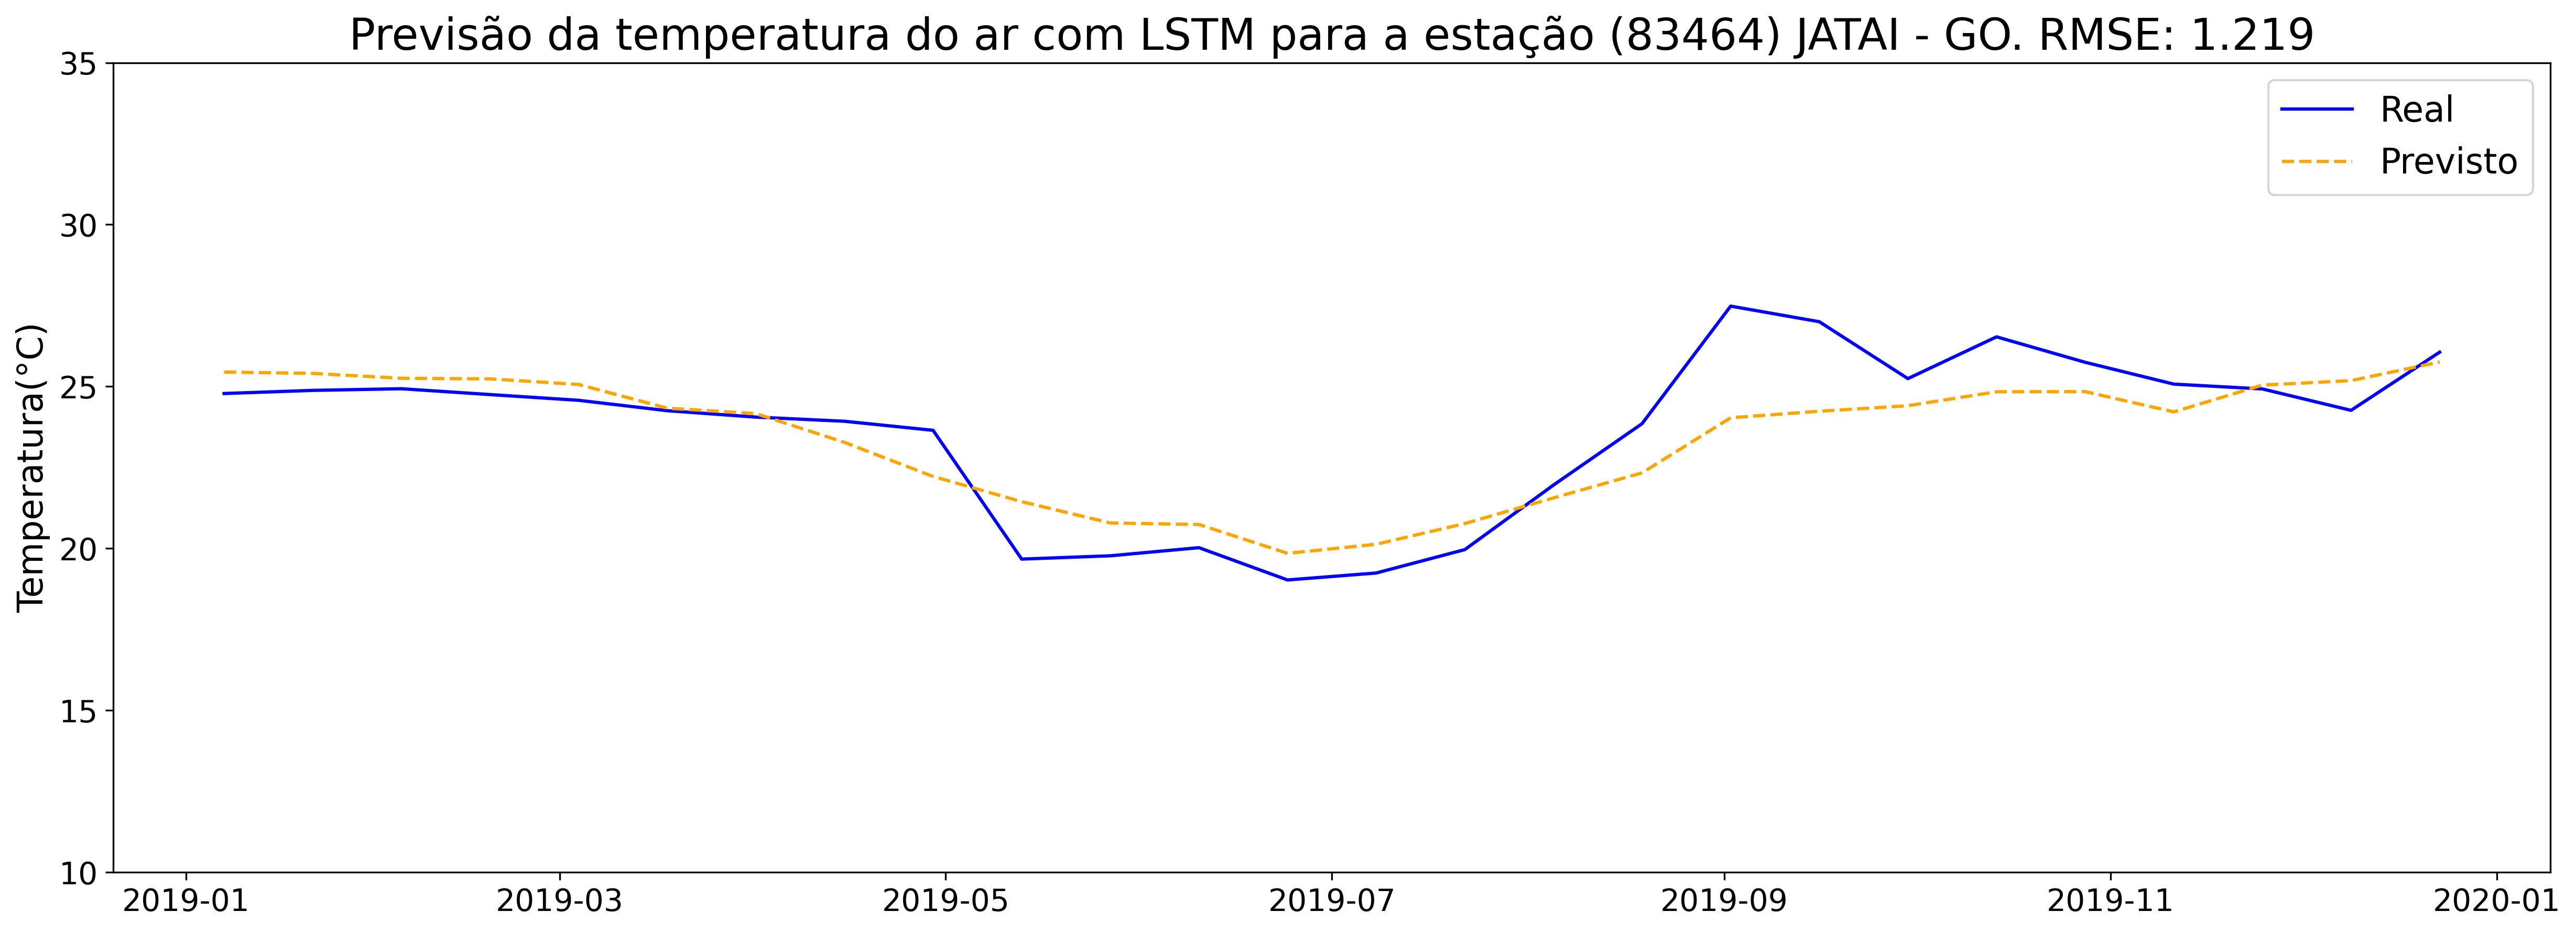
\includegraphics[scale=.30]{figuras/results/results_lstm_83464.png}}
\label{fig:results_lstm_83464}%
\end{figure}

\begin{figure}[H]%
\caption{Resultado da previsão da temperatura do ar para o ano de 2019 na estação meteorológica localizada no município de Cuiabá, no estado do Mato Grosso.}
\centering
\subfloat{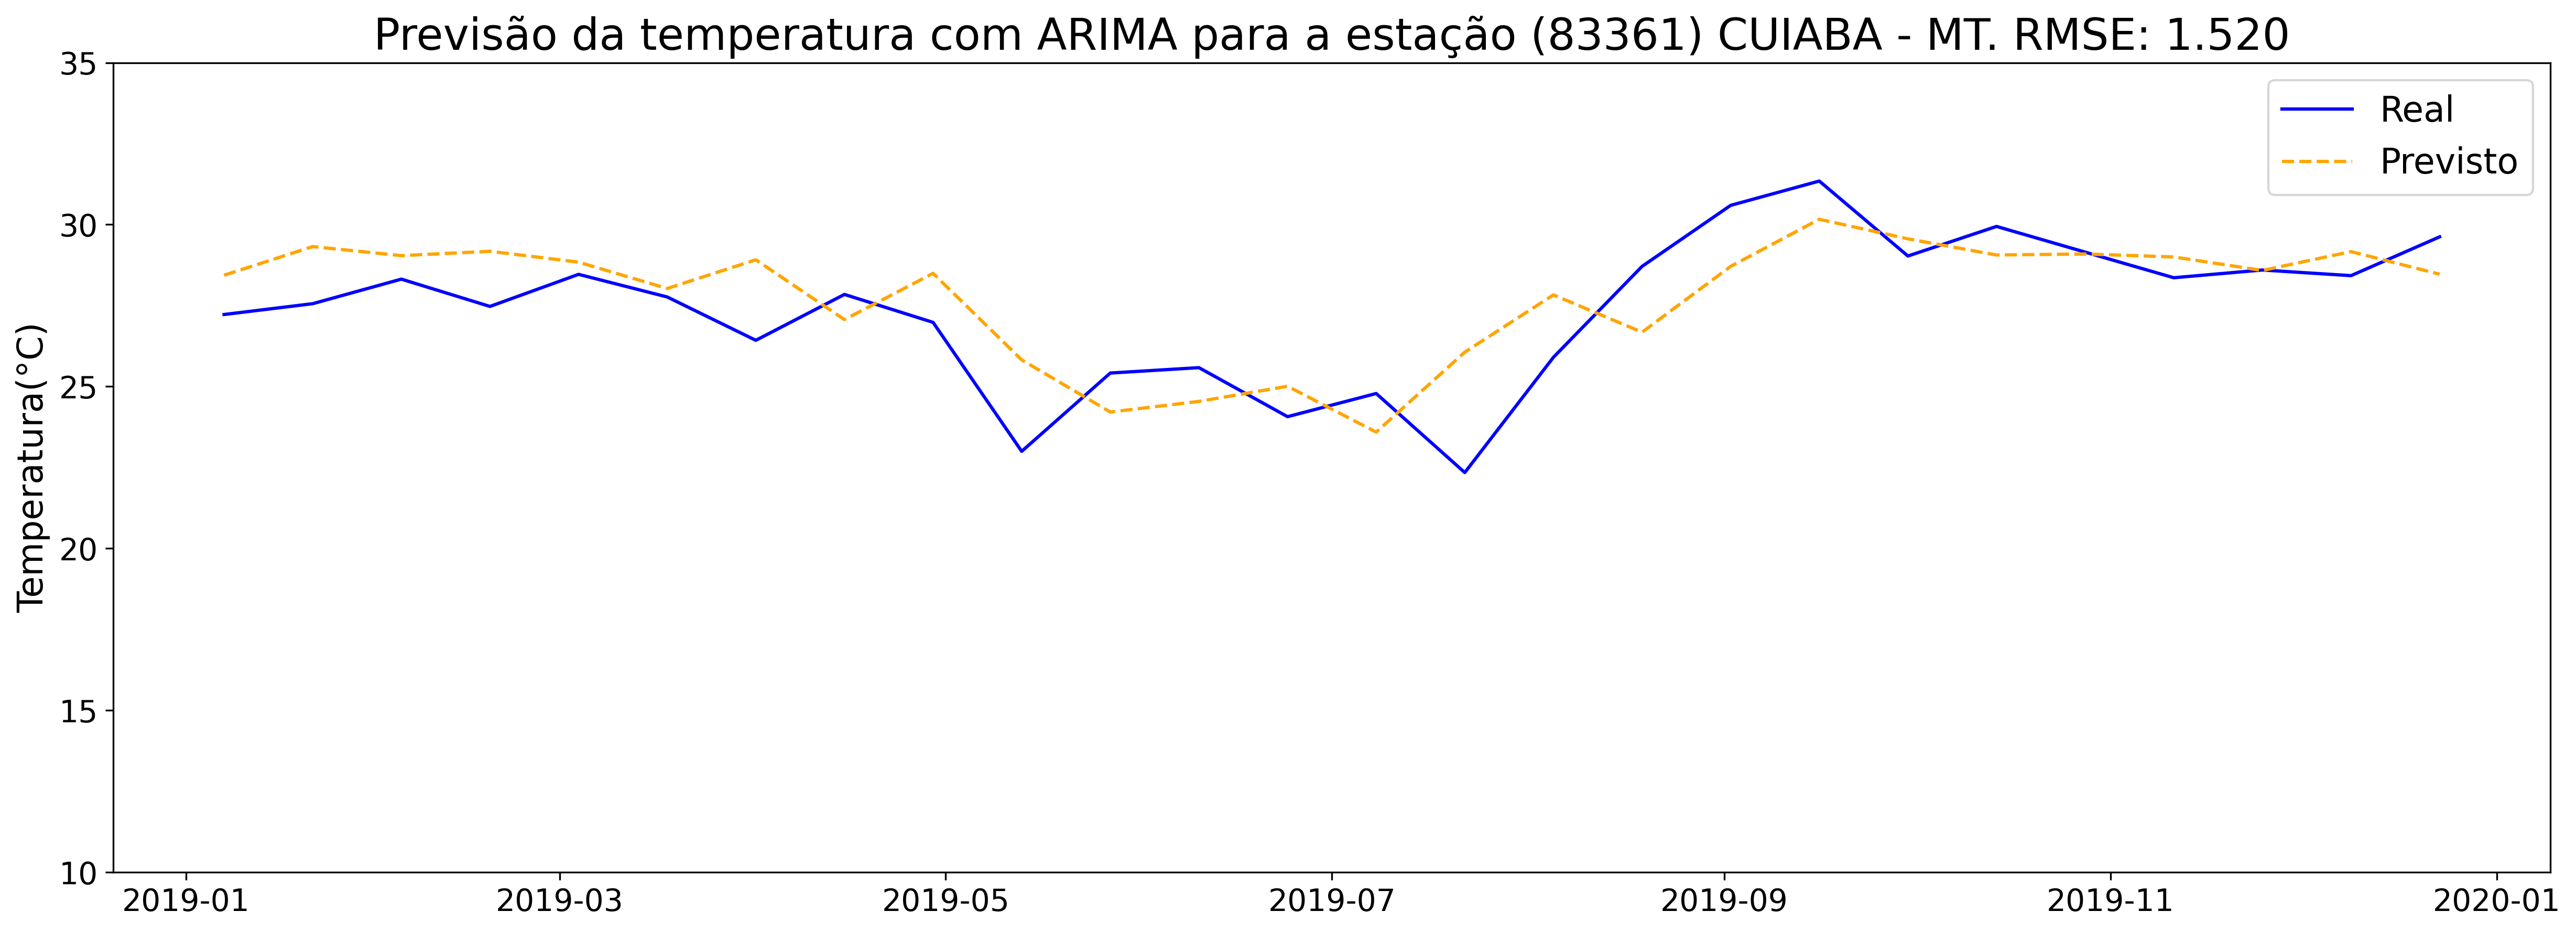
\includegraphics[scale=.30]{figuras/results/results_arima_83361.png}}
\qquad
\subfloat{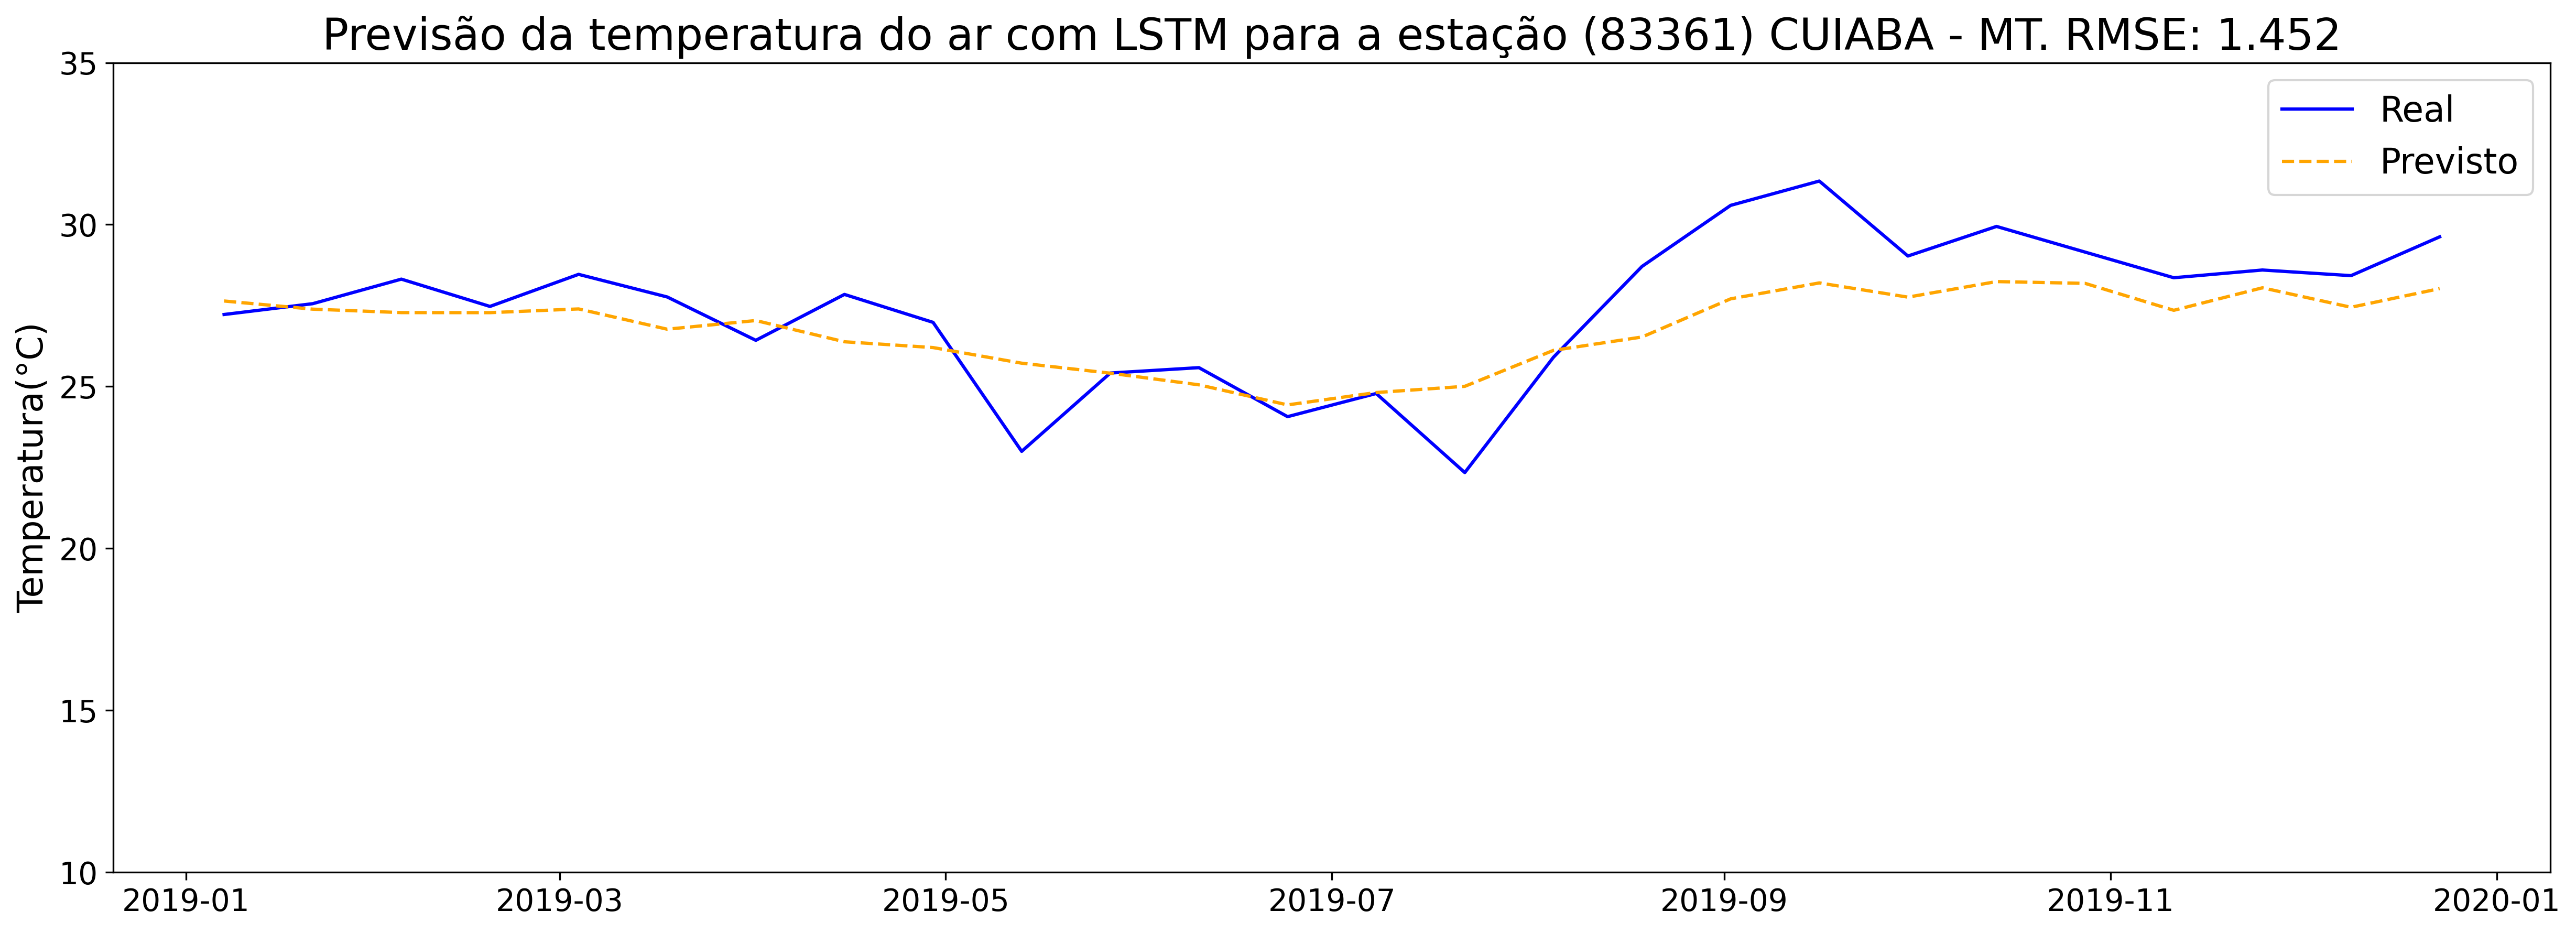
\includegraphics[scale=.30]{figuras/results/results_lstm_83361.png}}
\label{fig:results_lstm_83361}%
\end{figure}

\renewcommand{\cleardoublepage}{}
\renewcommand{\clearpage}{}
\vspace{5mm}
\chapter{Links}

Disponibilizamos os dados utilizados, scripts desenvolvidos e vídeo explicativo através dos links: 

\begin{itemize}
    \item Brazil Weather, Conventional Stations (1961-2019):
    
    \href{https://www.kaggle.com/saraivaufc/conventional-weather-stations-brazil}{https://www.kaggle.com/saraivaufc/conventional-weather-stations-brazil}
    
    \item Brazil Weather, Automatic Stations (2000-2019):
    
    \href{https://www.kaggle.com/saraivaufc/automatic-weather-stations-brazil}{https://www.kaggle.com/saraivaufc/automatic-weather-stations-brazil}
    
    \item LabMet - Automatic Weather Stations (2007-2019):
    
    \href{https://www.kaggle.com/saraivaufc/automatic-weather-stations-labmet}{https://www.kaggle.com/saraivaufc/automatic-weather-stations-labmet}
    
    \item Scripts desenvolvidos: \href{https://github.com/saraivaufc/TCC-Ciencia-de-Dados}{https://github.com/saraivaufc/TCC-Ciencia-de-Dados}
    
    \item Vídeo com explicação sobre este trabalho: \href{https://youtu.be/gYE2-oue06Y}{https://youtu.be/gYE2-oue06Y}
\end{itemize}


\newpage

\referencias{elementos-pos-textuais/Bibliografia}


\end{document}

